\chapter{量子色动力学}\label{chap:qcd}

QED 的局域 $U(1)$ 对称只作用在带电场的复相位上。强相互作用需要的内部空间更大。这里\emph{夸克味}（flavor）指 $u,d,s,c,b,t$ 这类具有相同颜色表示、但质量和弱相互作用量子数参数不同的夸克种类；味指标记为 $f$。对每一种夸克味，Dirac 场还带一个独立的颜色指标
\begin{equation*}
 \psi_f(x)
 =\begin{pmatrix}
 \psi_f^1(x)&\psi_f^2(x)&\cdots&\psi_f^{N_c}(x)
 \end{pmatrix}^{\!T},
 \qquad \psi_f(x)\in V_F\cong\mathbb C^{N_c}.
\end{equation*}
颜色基底本身不可观测，因此物理规律不能依赖在 $V_F$ 中怎样选择一组正交基。保持厄米内积并去除整体相位后的基变换构成 $SU(N_c)$。以下群论和规范论先保持一般 $N_c$；真实 QCD 在一般公式建立后取 $N_c=3$，此时一组方便的颜色基常称为红、绿、蓝。

同一个“夸克”一词在场论计算和实验图像中对应不同层级，先把它们分开会减少后面的概念负担。$\psi_f^i(x)$ 是\emph{量子场算符}的颜色分量；量子化以后，相应产生算符作用在真空上产生夸克或反夸克的一粒子激发。规范联络写成 $\mathscr C_\mu^a(x)$，其中 $a=1,\ldots,N_c^2-1$ 是伴随表示指标；它的单量子激发称为\emph{胶子}。微扰散射图的外线表示用来定义短距离振幅的渐近在壳夸克或胶子态，内部线则是传播子的积分核，一般不满足外部质量壳条件。真正到达探测器的强相互作用末态通常是颜色单态的\emph{强子}（hadron）以及由许多强子形成的\emph{喷注}（jet）。因此短距离计算中把夸克、胶子统称为\emph{部分子}（parton）：它们不是把自由夸克当成可直接探测粒子，而是把硬散射与随后不可微扰的强子化分层描述。

局域化颜色基变换会迫使一个新的数学对象出现。若 $U=U(x)\in SU(N_c)$，普通导数作用于 $U(x)\psi_f(x)$ 时会产生 $\partial_\mu U$，因此必须引入矩阵值协变导数。由于 $SU(N_c)$ 的生成元不对易，协变导数的曲率除了导数项还含 $[\mathscr C_\mu,\mathscr C_\nu]$。这一项在作用量中产生三胶子和四胶子相互作用；量子化后，相互作用作用量的三次、四次场项分别给出相应 Feynman 顶角。Dyson 展开到高阶后，内部场的 Wick 收缩形成闭合传播链；顶角四动量守恒不能固定的独立内部四动量成为圈动量积分，因此相应高阶项表现为圈图。

由此，QCD 的各层结构可以从同一个局域对称性连续推出：$SU(N_c)$ 的生成元和群不变量进入协变导数，协变导数的曲率给出 Yang--Mills 场强，作用量的二次项决定传播子而三次、四次项决定胶子自耦合顶角。树级部分子振幅由这些顶角直接组成；圈积分再产生耦合常数的尺度运行，而因子化把短距离部分子计算与长距离强子化分开。$N_c=3$ 只在需要真实 QCD 数值时才代入，因此 $C_F,C_A,T_F$、三胶子自耦合和一圈 $\beta$ 函数始终可以追溯到同一套群论结构。

\section{非阿贝尔规范联络与 QCD 的颜色实现}\label{sec:qcd-group-gauge-dp10}

QED 中局域相位变换 $\psi(x)\to \ee^{\ii\alpha(x)}\psi(x)$ 使 $\partial_\mu\psi$ 多出 $\partial_\mu\alpha$，协变导数用一个四势恰好补偿这项。现在唯一改变的是：夸克的内部态不再是一维复相位，而是 $N_c$ 维颜色向量，局域基变换 $U(x)$ 是矩阵。因此在引入规范场之前，必须先把三个对象区分清楚：颜色向量属于哪个表示、无穷小基变换由哪些生成元产生、平方振幅里会出现哪些基底无关的群不变量。

这些对象一旦定义，局域化步骤与 QED 完全平行：先要求 $D_\mu'\psi'=UD_\mu\psi$ 来确定矩阵值联络的变换律，再用 $[D_\mu,D_\nu]$ 定义曲率，最后用曲率平方构造规范场动能。非阿贝尔新物理只出现在一个地方——生成元不对易——但它会连续传递到场强、顶角、颜色因子和一圈运行中。全过程先保持一般 $SU(N_c)$，物理 QCD 的 $N_c=3$ 只在一般结果建立以后代入。

\subsection{颜色表示与 $SU(N_c)$ 群不变量}

把一个夸克的颜色分量记为列向量 $q^i$，$i=1,\ldots,N_c$。颜色空间本身是一个带厄米内积的复向量空间 $V_F\cong\mathbb C^{N_c}$；选择一组基底以后，基变换写成 $q\mapsto Uq$。保持内积要求 $U^\dagger U=I$，再去掉整体行列式相位后得到
\begin{equation}
 \boxed{
 SU(N_c)=\{U\in\mathbb C^{N_c\times N_c}\mid U^\dagger U=I_{N_c},\ \det U=1\}.}
 \label{eq:SUN-definition-dp10}
\end{equation}
这个 $N_c$ 维作用空间称为\emph{基本表示} $F$。物理 QCD 的夸克属于 $F$，但群论推导暂时不取 $N_c=3$。

生成元最好直接由群曲线在恒等元处的切向量定义。对第 $a$ 个一参数子群
\begin{equation*}
 U_a(\tau)=\exp(\ii\tau T^a),
 \qquad U_a(0)=I,
 \qquad
 \left.\frac{\dd U_a}{\dd\tau}\right|_{\tau=0}=\ii T^a .
\end{equation*}
对恒等式 $U_a^\dagger U_a=I$ 在 $\tau=0$ 求导，得到
\begin{equation*}
 -\ii T^{a\dagger}+\ii T^a=0,
 \qquad\Longrightarrow\qquad T^{a\dagger}=T^a.
\end{equation*}
再用 Jacobi 行列式公式
\begin{equation*}
 \left.\frac{\dd}{\dd\tau}\det U_a(\tau)\right|_{0}
 =\det U_a(0)\,
 \Tr\!\left[U_a^{-1}(0)\left.\frac{\dd U_a}{\dd\tau}\right|_0\right]
 =\ii\Tr T^a,
\end{equation*}
而 $\det U_a(\tau)=1$ 对所有 $\tau$ 恒成立，所以 $\Tr T^a=0$。厄米 $N_c\times N_c$ 矩阵有 $N_c^2$ 个实参数，去掉迹方向后得到 $N_c^2-1$ 个独立生成方向；物理 $SU(3)$ 因而有八个伴随颜色方向，量子化相应规范联络后得到八个胶子场分量。

平方振幅不会依赖某一套显式生成元矩阵，而只会出现诸如 $\Tr(T^aT^b)$、$\sum_aT^aT^a$ 和 $f^{acd}f^{bcd}$ 这样的基底无关组合。为此先固定生成元归一化，再定义后面颜色求和真正需要的三个群不变量 $T_F,C_F,C_A$。

在基本表示中取厄米无迹生成元 $T^a$，$a=1,\ldots,N_c^2-1$。第一章已经说明，生成元整体归一化必须先作为约定固定；粒子物理采用
\begin{equation}
 \boxed{
 \Tr_F(T^aT^b)=T_F\delta^{ab},
 \qquad T_F\equiv T(F)=\frac12.}
 \label{eq:SUN-generator-normalization-dp10}
\end{equation}
在这一约定下，Lie 括号写成
\begin{equation}
 \boxed{
 [T^a,T^b]=\ii f^{abc}T^c,}
 \label{eq:SUN-commutator-dp10}
\end{equation}
其中 $f^{abc}$ 为实的完全反对称结构常数。非零 $f^{abc}$ 固定了后面三胶子、四胶子相互作用的代数系数；相应 Feynman 顶角随后由 Yang--Mills 作用量展开得到。

生成元不仅可以作用在夸克的基本表示空间上，也可以作用在 Lie 代数自身。把一个 Lie 代数元素写成 $X=X^bT^b$，无穷小群变换给出
\begin{equation*}
 \delta X=\ii\theta^a[T^a,X]
 =-\theta^af^{abc}X^bT^c.
\end{equation*}
因此 Lie 代数分量 $X^b$ 本身构成一个 $N_c^2-1$ 维表示，其生成元可取
\begin{equation*}
 (T_{\rm Adj}^a)_{cb}=-\ii f^{abc}.
\end{equation*}
这个表示称为\emph{伴随表示}。胶子场 $\mathscr C_\mu^a$ 的颜色指标 $a$ 正是伴随表示指标；所以物理 $SU(3)$ 中有 $3^2-1=8$ 个胶子颜色方向。

在进入 Casimir 以前，还需要固定另一个常见群论系数。对表示 $R$ 的生成元定义迹归一化
\begin{equation*}
 \Tr_R(T_R^aT_R^b)\equiv T(R)\delta^{ab}.
\end{equation*}
这里的 $T(R)$ 称为表示 $R$ 的 Dynkin 指标（更准确地说是生成元的迹归一化指数）：它衡量在该表示中两个生成元做迹以后留下的统一系数。取基本表示归一化 $T(F)=1/2$。它与随后定义的二次 Casimir 是两个相关但不同的数：$T(R)$ 来自“两个生成元的迹”，$C_2(R)$ 来自“全部生成元平方之和”。

这里首次出现的\emph{二次 Casimir} 是表示本身的一个基底无关数字。对任意不可约表示 $R$，把该表示中的全部生成元平方求和，定义
\begin{equation*}
 \mathcal C_2(R)\equiv\sum_a T_R^aT_R^a.
\end{equation*}
由 Lie 代数对易关系可验证 $[\mathcal C_2(R),T_R^b]=0$；Schur 引理于是给出 $\mathcal C_2(R)=C_2(R)I_R$。也就是说，$C_2(R)$ 只取决于“粒子处在哪个群表示”，不取决于我们怎样选颜色基。基本表示上的数记为 $C_F$，伴随表示上的数记为 $C_A$；后者就是胶子颜色求和反复出现的群论系数。

基本表示与伴随表示的 Casimir 要分别从各自的表示数据得到。对基本表示，一般恒等式\eqnrefs{eq:casimir-dynkin-relation-dp11}
\[
 d_R C_2(R)=d_G T(R)
\]
与
\[
 d_F=N_c,\qquad d_G=N_c^2-1,\qquad T(F)=\frac12
\]
直接给出
\begin{equation}
 \sum_aT^aT^a=C_FI_{N_c},
 \qquad
 C_F=\frac{N_c^2-1}{2N_c}.
 \label{eq:CF-definition-dp10}
\end{equation}

胶子处在伴随表示，因而不能把上面的基本表示维数代入再次使用。伴随表示生成元为
\[
 (F^a)_{bc}=-\ii f^{abc},
\]
而第一章已经由 $SU(N_c)$ 的伴随表示结构得到
$C_2(\mathrm{Adj})=N_c$，即正文\eqnrefs{eq:ca-general-math-dp11}。于是伴随表示的 Casimir 定义
\[
 \sum_c(F^cF^c)_{ab}=C_A\delta_{ab}
\]
左端逐个写开为
\begin{align*}
 \sum_{c,d}(F^c)_{ad}(F^c)_{db}
 &=-\sum_{c,d}f^{cad}f^{cdb}\\
 &=\sum_{c,d}f^{acd}f^{bcd},
\end{align*}
其中第二行只用了结构常数的全反对称性和哑指标重命名。因此
\begin{equation}
 f^{acd}f^{bcd}=C_A\delta^{ab},
 \qquad C_A=N_c.
 \label{eq:CA-definition-dp10}
\end{equation}
因此
\begin{equation}
 \boxed{
 C_F=\frac{N_c^2-1}{2N_c},
 \qquad C_A=N_c.}
 \label{eq:SUN-CF-CA-dp32}
\end{equation}
同样，第一章已经证明的 $SU(N_c)$ 基本表示完备关系在颜色指标上写成
\begin{equation}
 \boxed{
 \sum_{a=1}^{N_c^2-1}(T^a)_{ij}(T^a)_{kl}
 =T_F\left(\delta_{il}\delta_{jk}-\frac1{N_c}\delta_{ij}\delta_{kl}\right).}
 \label{eq:SUN-fierz-dp10}
\end{equation}
这些式子构成后面颜色求和的全部基础；QCD 再取 $N_c=3$，最后才得到
\[
T_F=\frac12,\qquad C_F=\frac43,\qquad C_A=3.
\]
$T_F$ 控制基本表示闭合夸克线的迹归一化，$C_F$ 控制单条夸克线的二次颜色荷，而 $C_A$ 控制伴随表示胶子的非阿贝尔颜色荷。

颜色因子还决定两体颜色通道的短程相互作用。对夸克--反夸克系统，
\begin{equation*}
 F\otimes\bar F=\mathbf1\oplus\mathrm{Adj},
\end{equation*}
总生成元 $\mathbf T=\mathbf T_1+\mathbf T_2$ 给出
\begin{equation}
 \mathbf T_1\!\cdot\!\mathbf T_2
 =\frac12\bigl[C_2(R)-2C_F\bigr].
 \label{eq:qcd-two-body-color-casimir-dp73}
\end{equation}
因此单胶子交换的短程静态势可写成
\begin{equation*}
 V_R(r)=\frac{\alpha_s\hbar c}{r}\,
 \mathbf T_1\!\cdot\!\mathbf T_2.
\end{equation*}
取 $SU(3)$ 后，颜色单态有 $\mathbf T_1\!\cdot\!\mathbf T_2=-4/3$，八重态有 $+1/6$。这个 Coulomb 型势只属于 $r\ll\lambda_{\rm QCD}=\hbar/\Lambda_{\rm QCD}$ 的微扰短程区；当运行耦合不再提供小参数时，必须转向 Wilson 环等非微扰规范不变量。

\begin{figure}[htbp]
 \centering
 
\includegraphics[width=.76\linewidth]{qcd_color_factors_dp18.png}
 \caption{先保留 $SU(N_c)$ 的一般颜色不变量，再在末端取 $N_c=3$。在固定 $T_F=1/2$ 的归一化下，$C_A=N_c$，而 $C_F=(N_c^2-1)/(2N_c)$。}
 \label{fig:qcd-color-factors-dp18}
\end{figure}

\figref{fig:qcd-color-factors-dp18} 把一般 $SU(N_c)$ 的两个 Casimir 随 $N_c$ 的变化画在同一坐标中。读图时应先看 $C_A=N_c$ 的线性增长，再比较 $C_F=(N_c^2-1)/(2N_c)$；$N_c=3$ 对应两条一般曲线上的物理 QCD 取值点。

\begin{note}[显式 $SU(3)$ 基底]
若需要显式矩阵，可以取 $T^a=\lambda^a/2$，其中 $\lambda^a$ 是 $SU(3)$ 基本表示的一组标准厄米无迹基矩阵，通常称为 Gell--Mann 矩阵。实际散射计算优先使用 \eqnrefs{eq:SUN-generator-normalization-dp10,eq:SUN-fierz-dp10,eq:SUN-CF-CA-dp32} 的基底无关恒等式，而不是逐个矩阵相乘。
\end{note}

\begin{exbox}[三种颜色与 $\Delta^{++}$ 的 Pauli 约束]
在最简单的夸克模型中，$\Delta^{++}$ 的三个价夸克都是 $u$。基态空间波函数对交换对称，自旋 $3/2$ 态的自旋波函数也对称，味部分同样对称。三个相同费米子的总态必须反对称，因此还需要一个反对称内部因子。物理 QCD 取 $N_c=3$ 时，颜色空间存在完全反对称单态
\begin{equation*}
 |1\rangle_{\rm color}
 =\frac1{\sqrt{3!}}\epsilon_{ijk}|i\rangle|j\rangle|k\rangle,
 \qquad i,j,k=1,2,3.
\end{equation*}
它与对称的空间、味和自旋部分相乘后使总费米子态满足 Pauli 原理。这个例子说明为什么三维颜色空间与强子谱相容；真正的 QCD 动力学还需要进一步把颜色基变换提升为局域 $SU(3)$ 对称，从而得到规范联络和胶子。
\end{exbox}

\subsection{局域颜色对称}

取味指标为 $f$ 的 Dirac 夸克场 \(\psi_f(x)\)，它同时携带 Dirac 旋量指标和颜色指标。由于全文已经用 \(q^\mu\) 表示四动量转移，夸克场统一记作 \(\psi_f\)。自由动能项为
\begin{equation}
 \Lag_{f,0}=\bar\psi_f(\ii\hbar c\gamma^\mu\partial_\mu-m_fc^2)\psi_f.
 \label{eq:free-quark-lagrangian-dp10}
\end{equation}
对常数 \(U\in SU(N_c)\)，变换 \(\psi_f\to U\psi_f\) 满足 \(\partial_\mu U=0\)，因而自由动能项保持不变。若颜色旋转依赖时空位置，即 \(U=U(x)\)，则
\begin{equation*}
 \partial_\mu \psi_f'
 =(\partial_\mu U)\psi_f+U\partial_\mu \psi_f,
\end{equation*}
第一项破坏局域协变性。与 QED 相同，需要引入规范联络；这里的联络是颜色矩阵：
\begin{equation*}
 \mathscr C_\mu(x)
 \equiv\mathscr C_\mu^a(x)T^a,
 \qquad
 D_\mu\equiv\partial_\mu+\ii g_s\mathscr C_\mu.
\end{equation*}
其中 \(g_s\) 是无量纲强规范耦合，
\begin{equation}
 \alpha_s\equiv\frac{g_s^2}{4\pi}.
 \label{eq:alpha-s-definition-dp10}
\end{equation}
为保持全文 SI 量纲显式，规范联络采用几何归一化
\begin{equation*}
 [\mathscr C_\mu]=\mathrm{m^{-1}},
 \qquad [D_\mu]=\mathrm{m^{-1}}.
\end{equation*}
这与电磁四势 \(A_\mu\) 的 \(\mathrm{V\,s\,m^{-1}}\) 归一化不同，因此使用花体 \(\mathscr C_\mu^a\) 避免混淆。

要求
\begin{equation}
 D_\mu'\psi_f'=U D_\mu\psi_f
 \label{eq:qcd-covariance-requirement-dp10}
\end{equation}
并代入 \(\psi_f'=U\psi_f\)：
\begin{align*}
 (\partial_\mu+\ii g_s\mathscr C_\mu')U\psi_f
 &=(\partial_\mu U)\psi_f+U\partial_\mu\psi_f
 +\ii g_s\mathscr C_\mu'U\psi_f,\\
 U(\partial_\mu+\ii g_s\mathscr C_\mu)\psi_f
 &=U\partial_\mu\psi_f+\ii g_sU\mathscr C_\mu\psi_f.
\end{align*}
逐项比较并右乘 \(U^{-1}\)，得到
\begin{equation}
 \boxed{
 \mathscr C_\mu'
 =U\mathscr C_\mu U^{-1}
 +\frac{\ii}{g_s}(\partial_\mu U)U^{-1}.}
 \label{eq:qcd-gauge-field-transformation-dp10}
\end{equation}
与阿贝尔情形相比，第一项不再等于原来的 $\mathscr C_\mu$，因为一般有 $[U,\mathscr C_\mu]\neq0$。这说明规范联络本身也携带颜色结构。

局域颜色空间在不同的时空点并没有天然的统一基底。比较 $y$ 点与 $x$ 点的颜色方向需要沿一条路径 $C:y\to x$ 做平行移动。一般联络的 Wilson 线由\eqnrefs{eq:wilson-line-general-dp11} 定义；在 QCD 基本表示中取联络 $g_s\mathscr C_\mu^aT^a$，于是端点变换律为
\begin{equation*}
 \mathcal W_C(x,y)\longrightarrow
 U(x)\mathcal W_C(x,y)U^{-1}(y).
\end{equation*}
因此两点夸克算符
\begin{equation*}
 \bar\psi(x)\,\mathcal W_C(x,y)\,\psi(y)
\end{equation*}
可以构成局域规范不变量。规范联络沿有限路径的平行输运定义 Wilson 线；它是局域颜色协变性的积分形式。后面讨论强子的非局域双点算符、软辐射和高能散射时都会再次遇到同一个对象；相应的“部分子分布”等专门名称到实际定义这些可观测结构时再引入。

\subsection{场强与 QCD 作用量}

协变导数解决了“相邻时空点的颜色向量怎样比较”的问题；沿两个无穷小方向依次平行移动时，次序差则测量联络的曲率。QED 的一维内部相位使联络彼此对易，而 $SU(N_c)$ 联络为矩阵，因此同一个曲率定义会多出联络对易子。这个对易子随后进入曲率平方，自动生成胶子自相互作用。

QCD 场强由非阿贝尔协变导数的曲率定义。基本表示中的协变导数写成
\begin{equation}
\boxed{
D_\mu=\partial_\mu+i g_s\mathscr C_\mu,
\qquad
\mathscr C_\mu=\mathscr C_\mu^aT^a.}
\label{eq:qcd-covariant-derivative-dp68}
\end{equation}
两次协变微分的次序差定义曲率，约定
\begin{equation}
\boxed{
[D_\mu,D_\nu]=i g_s\mathcal F_{\mu\nu}.}
\label{eq:qcd-curvature-definition-dp68}
\end{equation}
把\eqnrefs{eq:qcd-covariant-derivative-dp68} 展开到\eqnrefs{eq:qcd-curvature-definition-dp68}，得到
\begin{equation}
\boxed{
\mathcal F_{\mu\nu}
=\partial_\mu\mathscr C_\nu-\partial_\nu\mathscr C_\mu
+i g_s[\mathscr C_\mu,\mathscr C_\nu],}
\label{eq:qcd-field-strength-matrix-dp10}
\end{equation}
或分量形式
\begin{equation*}
\mathcal F_{\mu\nu}^a
=\partial_\mu\mathscr C_\nu^a-\partial_\nu\mathscr C_\mu^a
-g_sf^{abc}\mathscr C_\mu^b\mathscr C_\nu^c.
\end{equation*}
最后一项由李代数生成元不对易直接产生；把它代入曲率平方后便得到胶子的三点与四点自相互作用。

在局域规范变换下 $D'_\mu=UD_\mu U^{-1}$，因此曲率按 $\mathcal F'_{\mu\nu}=U\mathcal F_{\mu\nu}U^{-1}$ 协变变换。矩阵值场强本身不是规范不变量，但迹的循环性质保证 $\operatorname{Tr}(\mathcal F_{\mu\nu}\mathcal F^{\mu\nu})$ 不变。对 $n_f$ 个夸克味，满足局域性、Lorentz 不变性与可重整化性的最小 QCD 拉格朗日量在 SI 约定下为
\begin{equation}
\boxed{
\mathcal L_{\rm QCD}
=\sum_{f=1}^{n_f}\bar\psi_f(\ii\hbar c\gamma^\mu D_\mu-m_fc^2)\psi_f
-\frac{\hbar c}{4}\mathcal F_{\mu\nu}^a\mathcal F^{a\mu\nu}.}
\label{eq:qcd-lagrangian-si-dp10}
\end{equation}
第一项描述夸克在颜色联络中的传播；第二项是规范曲率构成的最低阶 Lorentz 标量动能项。

展开夸克协变导数得到
\begin{equation}
\mathcal L_{qg}
=-\hbar c\,g_s\bar\psi_f\gamma^\mu T^a\psi_f\,\mathscr C_\mu^a,
\label{eq:qcd-quark-gluon-interaction-dp10}
\end{equation}
所以夸克--胶子顶角等于阿贝尔矢量流顶角乘上颜色生成元。另一方面，\eqnrefs{eq:qcd-field-strength-matrix-dp10} 的非线性部分使纯规范场动能自动包含 $\mathscr C$ 的三次与四次项：
\begin{align}
-\frac{\hbar c}{4}\mathcal F^2
={}&-\frac{\hbar c}{4}\mathcal F_{\mu\nu}^{a(0)}\mathcal F^{a(0)\mu\nu}
+\frac{\hbar c g_s}{2}f^{abc}\mathcal F_{\mu\nu}^{a(0)}\mathscr C^{b\mu}\mathscr C^{c\nu}\notag\\
&-\frac{\hbar c g_s^2}{4}f^{abc}f^{ade}
\mathscr C_\mu^b\mathscr C_\nu^c\mathscr C^{d\mu}\mathscr C^{e\nu},
\label{eq:yang-mills-expanded-3-4-gluon-dp10}
\end{align}
其中 $\mathcal F_{\mu\nu}^{a(0)}=\partial_\mu\mathscr C_\nu^a-\partial_\nu\mathscr C_\mu^a$。三胶子与四胶子顶角因此是局域非阿贝尔对称性的直接后果。

\begin{derivation}[从\eqnrefs{eq:qcd-covariant-derivative-dp68}到\eqnrefs{eq:qcd-field-strength-matrix-dp10}]
让 $[D_\mu,D_\nu]$ 作用在任意基本表示颜色场 $\chi$ 上。由于 $D_\mu$ 含微分算符，必须先完成对场的作用，再比较两种作用次序：

\begin{align*}
D_\mu D_\nu\chi
={}&\partial_\mu\partial_\nu\chi
+i g_s(\partial_\mu\mathscr C_\nu)\chi
+i g_s\mathscr C_\nu\partial_\mu\chi\\
&+i g_s\mathscr C_\mu\partial_\nu\chi
-g_s^2\mathscr C_\mu\mathscr C_\nu\chi,
\end{align*}
而交换 $\mu\leftrightarrow\nu$ 得
\begin{align*}
D_\nu D_\mu\chi
={}&\partial_\nu\partial_\mu\chi
+i g_s(\partial_\nu\mathscr C_\mu)\chi
+i g_s\mathscr C_\mu\partial_\nu\chi\\
&+i g_s\mathscr C_\nu\partial_\mu\chi
-g_s^2\mathscr C_\nu\mathscr C_\mu\chi.
\end{align*}
普通偏导彼此对易，且两组含 $\partial\chi$ 的交叉项逐项相消，所以
\begin{equation*}
[D_\mu,D_\nu]\chi
=\left\{i g_s(\partial_\mu\mathscr C_\nu-\partial_\nu\mathscr C_\mu)
-g_s^2[\mathscr C_\mu,\mathscr C_\nu]\right\}\chi.
\end{equation*}
提出 $i g_s$ 就得到\eqnrefs{eq:qcd-field-strength-matrix-dp10}。再写
\begin{equation*}
\mathscr C_\mu=\mathscr C_\mu^aT^a,
\qquad
[\mathscr C_\mu,\mathscr C_\nu]
=i f^{abc}\mathscr C_\mu^a\mathscr C_\nu^bT^c,
\end{equation*}
便得到分量形式中的 $-g_sf^{abc}\mathscr C_\mu^b\mathscr C_\nu^c$。
\end{derivation}

\begin{derivation}[从\eqnrefs{eq:qcd-field-strength-matrix-dp10}到\eqnrefs{eq:yang-mills-expanded-3-4-gluon-dp10}]
纯规范场部分的三次与四次相互作用可以从场强平方直接展开。定义

\begin{equation*}
\mathcal F_{\mu\nu}^{a(0)}\equiv
\partial_\mu\mathscr C_\nu^a-\partial_\nu\mathscr C_\mu^a,
\qquad
X_{\mu\nu}^a\equiv f^{abc}\mathscr C_\mu^b\mathscr C_\nu^c,
\end{equation*}
则 $\mathcal F_{\mu\nu}^a=\mathcal F_{\mu\nu}^{a(0)}-g_sX_{\mu\nu}^a$。平方为
\begin{equation*}
\mathcal F_{\mu\nu}^a\mathcal F^{a\mu\nu}
=\mathcal F_{\mu\nu}^{a(0)}\mathcal F^{a(0)\mu\nu}
-2g_s\mathcal F_{\mu\nu}^{a(0)}X^{a\mu\nu}
+g_s^2X_{\mu\nu}^aX^{a\mu\nu}.
\end{equation*}
乘上 $-\hbar c/4$ 后，依次得到自由项、三次项与四次项。三次项的系数还需要利用场强的反对称结构整理：
\begin{align*}
\mathcal F_{\mu\nu}^{a(0)}X^{a\mu\nu}
&=f^{abc}(\partial_\mu\mathscr C_\nu^a-\partial_\nu\mathscr C_\mu^a)
\mathscr C^{b\mu}\mathscr C^{c\nu}.
\end{align*}
第二项交换哑 Lorentz 指标 $\mu\leftrightarrow\nu$ 后变为
\begin{equation*}
-f^{abc}(\partial_\mu\mathscr C_\nu^a)
\mathscr C^{b\nu}\mathscr C^{c\mu}.
\end{equation*}
再交换哑颜色指标 $b\leftrightarrow c$，并利用 $f^{acb}=-f^{abc}$，它变成与第一项相同的
\begin{equation*}
f^{abc}(\partial_\mu\mathscr C_\nu^a)
\mathscr C^{b\mu}\mathscr C^{c\nu}.
\end{equation*}
因此两项相加产生因子 $2$，三次拉氏量可写成
\begin{equation*}
\mathcal L_{3g}
=\hbar c g_s f^{abc}(\partial_\mu\mathscr C_\nu^a)
\mathscr C^{b\mu}\mathscr C^{c\nu},
\end{equation*}
这就是\eqnrefs{eq:yang-mills-expanded-3-4-gluon-dp10} 的交叉项。四次项为
\begin{equation*}
\mathcal L_{4g}
=-\frac{\hbar c g_s^2}{4}
 f^{abc}f^{ade}
 \mathscr C_\mu^b\mathscr C_\nu^c
 \mathscr C^{d\mu}\mathscr C^{e\nu}.
\end{equation*}

\end{derivation}



\subsection{鬼场与规范固定}

路径积分若直接遍历所有 $\mathscr C_\mu^a$，会把彼此只差一次局域颜色旋转的场构型重复计数；这些构型代表同一个物理状态。要得到可逆的二次核和正确的微扰展开，必须从每条规范轨道中选一个代表。以协变条件
\begin{equation*}
 G^a[\mathscr C]\equiv\partial^\mu\mathscr C_\mu^a=0
\end{equation*}
为例，关键问题是：一次无穷小规范变换会让 $G^a$ 改变多少？这个变化率决定从“沿规范轨道积分”换成“在规范切片上积分”时的 Jacobian。

把这一 Jacobian 写成
\begin{equation*}
 1=\Delta_{\rm FP}[\mathscr C]
 \int\mathcal D\theta\,
 \delta\!\left(G[\mathscr C^\theta]\right)
\end{equation*}
就是 Faddeev--Popov 恒等式；$\Delta_{\rm FP}$ 是上述规范轨道变量变换的泛函 Jacobian。为直接从无穷小轨道切向读取该 Jacobian，取一参数规范轨道
\begin{equation*}
 U_\tau(x)=\exp[-\ii\tau\theta^a(x)T^a],
 \qquad \mathscr C_\mu(\tau)=\mathscr C_\mu^{U_\tau}.
\end{equation*}
由有限变换律\eqnrefs{eq:qcd-gauge-field-transformation-dp10} 对 $\tau$ 在零点求导，定义轨道切向量
\begin{equation*}
 \left.\frac{\dd\mathscr C_\mu^a(\tau)}{\dd\tau}\right|_0
 =-\frac1{g_s}(D_\mu\theta)^a,
 \qquad
 (D_\mu\theta)^a
 =\partial_\mu\theta^a-g_sf^{abc}\mathscr C_\mu^b\theta^c.
\end{equation*}
于是规范条件沿轨道的 Fr\'echet 导数为
\begin{equation*}
 \left.\frac{\dd G^a[\mathscr C(\tau)](x)}{\dd\tau}\right|_0
 =-\frac1{g_s}\partial^\mu D_\mu^{ab}\theta^b(x).
\end{equation*}
把与规范场无关的常数 $1/g_s$ 从行列式归一化中提出，定义 Faddeev--Popov 算符
\begin{equation}
 \boxed{
 \mathcal M_{\rm FP}^{ab}(x,y)
 \equiv
 g_s\frac{\delta G^a(x)}{\delta\theta^b(y)}
 =-\partial_x^\mu D_\mu^{ab}(x)\,\delta^{(4)}(x-y).}
 \label{eq:qcd-fp-operator-dp10}
\end{equation}
在 QED 中，这个 Jacobian 与电磁场本身无关，通常可以并入整体归一化；这里的 $D_\mu^{ab}$ 却含有 $\mathscr C_\mu$，所以行列式会随规范场改变，不能丢掉。这个场依赖行列式可由 Grassmann 高斯积分表示为局域指数。引入一对反对易标量场 $c^a,\bar c^a$。Grassmann Gaussian 恒等式给出同一算符行列式；为消除与 $\mathscr C$ 无关的泛函测度常数，采用相对于零背景的归一化：
\begin{equation*}
 \boxed{
 \frac{\Delta_{\rm FP}[\mathscr C]}{\Delta_{\rm FP}[0]}
 =
 \frac{
 \displaystyle\int\mathcal D\bar c\,\mathcal Dc\,
 \exp\!\left[
 \ii\int\dd^4x\,\bar c^a(-\partial^\mu D_\mu^{ab})c^b
 \right]}
 {
 \displaystyle\int\mathcal D\bar c\,\mathcal Dc\,
 \exp\!\left[
 \ii\int\dd^4x\,\bar c^a(-\partial^2\delta^{ab})c^b
 \right]}.}
\end{equation*}
所以规范固定后的拉格朗日量包含
\begin{equation}
 \Lag_{\rm gf+gh}
 =-\frac{\hbar c}{2\xi}(\partial^\mu\mathscr C_\mu^a)^2
 +\hbar c\,\bar c^a(-\partial^\mu D_\mu^{ab})c^b.
 \label{eq:qcd-gauge-fixing-ghost-lagrangian-dp10}
\end{equation}
把伴随协变导数展开并对相互作用项分部积分，可把鬼场部分写成
\begin{equation}
\boxed{
\mathcal L_{\rm gh}
=-\hbar c\,\bar c^a\partial^2c^a
-\hbar c\,g_sf^{abc}(\partial^\mu\bar c^a)\mathscr C_\mu^b c^c.}
\label{eq:qcd-ghost-expanded-dp68}
\end{equation}
这两个场称为 Faddeev--Popov 鬼场。它们在 Lorentz 变换下是标量，却采用 Grassmann 反对易变量；这种“标量但反对易”的组合并不是新增一种可制备粒子，而是为了让 Grassmann 高斯积分精确产生规范轨道 Jacobian 的行列式。因而鬼场没有物理渐近外态，只能作为内部传播自由度进入微扰展开。\eqnrefs{eq:qcd-ghost-expanded-dp68} 的第二项给出鬼--反鬼--胶子耦合；在圈图中，它与协变量子化引入的非物理胶子偏振共同组成满足 Slavnov--Taylor 恒等式的规范不变组合。

\begin{figure}[htbp]
\centering
\begin{tikzpicture}[
 x=1cm,y=1cm,
 gluon/.style={draw,line width=0.75pt,decorate,decoration={coil,aspect=0.65,amplitude=1.0pt,segment length=4.2pt}},
 ghost/.style={draw,dashed,line width=0.7pt,postaction={decorate},decoration={markings,mark=at position 0.56 with {\arrow{Stealth[length=1.8mm,width=1.3mm]}}}}
]
% q q g
\begin{scope}[shift={(0,0)}]
 \node[font=\bfseries] at (0,1.45) {(a) quark--gluon};
 \coordinate (v) at (0,0);
 \draw[fermion] (-1.55,-0.75)--(v)--(1.55,-0.75);
 \draw[gluon] (v)--(0,1.0);
 \fill[fvertex] (v);
 \node[font=\small,anchor=west,fill=white,inner sep=1pt] at (0.24,0.58) {$a,\mu$};
\end{scope}
% 3g
\begin{scope}[shift={(4.3,0)}]
 \node[font=\bfseries] at (0,1.45) {(b) three-gluon};
 \coordinate (v) at (0,0);
 \draw[gluon] (v)--(-1.25,-0.82);
 \draw[gluon] (v)--(1.25,-0.82);
 \draw[gluon] (v)--(0,1.0);
 \fill[fvertex] (v);
 \node[font=\small,fill=white,inner sep=.8pt] at (-0.78,-0.12) {$a$};
 \node[font=\small,fill=white,inner sep=.8pt] at (0.78,-0.12) {$b$};
 \node[font=\small,anchor=west,fill=white,inner sep=.8pt] at (0.18,0.67) {$c$};
\end{scope}
% 4g
\begin{scope}[shift={(8.6,0)}]
 \node[font=\bfseries] at (0,1.45) {(c) four-gluon};
 \coordinate (v) at (0,0);
 \draw[gluon] (v)--(-1.1,-0.85);
 \draw[gluon] (v)--(1.1,-0.85);
 \draw[gluon] (v)--(-1.1,0.85);
 \draw[gluon] (v)--(1.1,0.85);
 \fill[fvertex] (v);
\end{scope}
% ghost gluon
\begin{scope}[shift={(2.15,-3.25)}]
 \node[font=\bfseries] at (0,1.35) {(d) ghost--gluon};
 \coordinate (v) at (0,0);
 \draw[ghost] (-1.55,-0.65)--(v)--(1.55,-0.65);
 \draw[gluon] (v)--(0,0.95);
 \fill[fvertex] (v);
 \node[font=\small,fill=white,inner sep=.8pt] at (-0.96,-0.72) {$\bar c^a$};
 \node[font=\small,fill=white,inner sep=.8pt] at (0.96,-0.72) {$c^c$};
\end{scope}
% contrast QED
\begin{scope}[shift={(6.55,-3.25)}]
 \node[font=\bfseries] at (0,1.35) {(e) Abelian reference};
 \draw[fermion] (-1.55,-0.65)--(0,-0.65)--(1.55,-0.65);
 \draw[photon] (0,-0.65)--(0,0.95);
 \fill[fvertex] (0,-0.65);
 \node[align=left,font=\small,anchor=west,fill=white,inner sep=1.5pt] at (0.68,0.32) {No QED tree vertices:\\$3\gamma,4\gamma,\bar c c\gamma$};
\end{scope}
\end{tikzpicture}

\caption{QCD 的基本微扰顶角。夸克--胶子、三胶子与四胶子顶角来自\eqnrefs{eq:qcd-lagrangian-si-dp10}；鬼场--胶子顶角来自规范固定的 Faddeev--Popov 行列式。}
\label{fig:qcd-elementary-vertices-dp10}
\end{figure}


局域 $SU(N_c)$ 对称性同时固定了三类微扰结构：$T^a$ 使夸克流携带颜色矩阵，$f^{abc}\neq0$ 使场强非线性并产生三胶子与四胶子顶角，而同一个非阿贝尔协变导数使 Faddeev--Popov 行列式依赖规范场并产生相互作用鬼场。由这些结构读出的传播子与顶角规则共同决定后续 QCD 散射振幅。


\begin{derivation}[从\eqnrefs{eq:qcd-gauge-field-transformation-dp10}到\eqnrefs{eq:qcd-ghost-expanded-dp68}]
取固定的 Lie 代数值函数 $\theta(x)=\theta^a(x)T^a$，并沿同一条规范轨道定义一参数曲线
\begin{equation*}
 U_\tau(x)=\exp[-\ii\tau\theta(x)],
 \qquad
 \mathscr C_\mu(\tau)
 =U_\tau\mathscr C_\mu U_\tau^{-1}
 +\frac{\ii}{g_s}(\partial_\mu U_\tau)U_\tau^{-1}.
\end{equation*}
在 $\tau=0$ 处有
\begin{equation*}
 \left.\frac{\dd U_\tau}{\dd\tau}\right|_0=-\ii\theta,
 \qquad
 \left.\frac{\dd U_\tau^{-1}}{\dd\tau}\right|_0=+\ii\theta .
\end{equation*}
对有限规范变换律直接求导：
\begin{align*}
 \left.\frac{\dd\mathscr C_\mu(\tau)}{\dd\tau}\right|_0
 &=-\ii[\theta,\mathscr C_\mu]
 +\frac1{g_s}\partial_\mu\theta\\
 &=\frac1{g_s}(D_\mu\theta)^aT^a,
\end{align*}
其中按照当前结构常数约定
\begin{equation*}
 (D_\mu\theta)^a
 =\partial_\mu\theta^a-g_sf^{abc}\mathscr C_\mu^b\theta^c.
\end{equation*}
若规范轨道参数采用反向曲线 $U_{-\tau}$，上式整体变号；以下把正文采用的轨道方向固定为
\begin{equation*}
 \delta_\theta\mathscr C_\mu^a
 \equiv
 \left.\frac{\dd\mathscr C_\mu^a(-\tau)}{\dd\tau}\right|_0
 =-\frac1{g_s}(D_\mu\theta)^a.
\end{equation*}
这只是对规范轨道坐标方向的定义，此后所有 Jacobian 都使用同一方向。

对 Lorenz 型规范函数
\begin{equation*}
 G^a[\mathscr C](x)=\partial^\mu\mathscr C_\mu^a(x),
\end{equation*}
其轨道导数为
\begin{equation*}
 \delta_\theta G^a(x)
 =-\frac1{g_s}\partial_x^\mu D_\mu^{ab}(x)\theta^b(x).
\end{equation*}
因此泛函导数严格等于
\begin{equation*}
 g_s\frac{\delta G^a(x)}{\delta\theta^b(y)}
 =-\partial_x^\mu D_\mu^{ab}(x)\delta^{(4)}(x-y)
 \equiv\mathcal M_{\rm FP}^{ab}(x,y),
\end{equation*}
即正文\eqnrefs{eq:qcd-fp-operator-dp10}。

在每条规范轨道与规范切片只有一个横截点的局部坐标片内，普通多维换元公式推广为
\begin{equation*}
 1=\Delta_{\rm FP}[\mathscr C]
 \int\mathcal D\theta\,\delta[G(\mathscr C^\theta)],
 \qquad
 \Delta_{\rm FP}[\mathscr C]=\det\mathcal M_{\rm FP},
\end{equation*}
其中与 $\mathscr C$ 无关的常数行列式已吸收到路径积分整体归一化。Grassmann Gaussian 恒等式给
\begin{equation*}
 \int\mathcal D\bar c\,\mathcal Dc\,
 \exp\!\left[
 \ii\int\dd^4x\,\bar c^a\mathcal M_{\rm FP}^{ab}c^b
 \right]
 =\mathcal N_{\rm gh}\det\mathcal M_{\rm FP},
\end{equation*}
其中 $\mathcal N_{\rm gh}$ 与背景规范场无关。把零背景值相除即可消去它：
\begin{equation*}
 \frac{\Delta_{\rm FP}[\mathscr C]}{\Delta_{\rm FP}[0]}
 =
 \frac{\displaystyle\int\mathcal D\bar c\,\mathcal Dc\,
 \ee^{\ii\int\dd^4x\,\bar c\mathcal M_{\rm FP}c}}
 {\displaystyle\int\mathcal D\bar c\,\mathcal Dc\,
 \ee^{\ii\int\dd^4x\,\bar c\mathcal M_{\rm FP}[0]c}}.
\end{equation*}
为了得到一般协变 $R_\xi$ 规范，引入辅助函数 $\omega^a(x)$ 以及归一化常数 $\mathcal N_\xi$，使
\begin{equation*}
 1=\mathcal N_\xi
 \int\mathcal D\omega\,
 \exp\!\left[-\frac{\ii}{2\xi}
 \int\dd^4x\,\omega^a\omega^a\right].
\end{equation*}
把 $\delta[G]$ 替换为 $\delta[G-\omega]$ 并先对 $\omega$ 积分，得到规范固定权重
\begin{equation*}
 \exp\!\left[-\frac{\ii}{2\xi}\int\dd^4x\,
 (\partial^\mu\mathscr C_\mu^a)^2\right],
\end{equation*}
对应
\begin{equation*}
 \mathcal L_{\rm gf}
 =-\frac{\hbar c}{2\xi}(\partial^\mu\mathscr C_\mu^a)^2.
\end{equation*}
与 Grassmann 行列式合并即得
\begin{equation*}
 \mathcal L_{\rm gf+gh}
 =-\frac{\hbar c}{2\xi}(\partial\!\cdot\!\mathscr C^a)^2
 +\hbar c\,\bar c^a(-\partial^\mu D_\mu^{ab})c^b.
\end{equation*}

最后展开伴随协变导数：
\begin{align*}
 \mathcal L_{\rm gh}
 &=\hbar c\,\bar c^a
 \left[-\partial^\mu
 \left(\partial_\mu c^a-g_sf^{abc}\mathscr C_\mu^bc^c\right)\right]\\
 &=-\hbar c\,\bar c^a\partial^2c^a
 +\hbar c g_sf^{abc}\bar c^a\partial^\mu(\mathscr C_\mu^bc^c).
\end{align*}
对第二项分部积分并取边界项为零：
\begin{equation*}
 \int\dd^4x\,\bar c^a\partial^\mu(\mathscr C_\mu^bc^c)
 =-\int\dd^4x\,(\partial^\mu\bar c^a)\mathscr C_\mu^bc^c.
\end{equation*}
于是
\begin{equation*}
 \boxed{
 \mathcal L_{\rm gh}
 =-\hbar c\,\bar c^a\partial^2c^a
 -\hbar c g_sf^{abc}(\partial^\mu\bar c^a)\mathscr C_\mu^bc^c,}
\end{equation*}
即正文\eqnrefs{eq:qcd-ghost-expanded-dp68}。第一项的逆核给鬼场传播子，第二项对 $\bar c,\mathscr C,c$ 的三阶泛函导数给鬼--反鬼--胶子顶角。
\end{derivation}


\section{微扰 QCD 与树级过程}\label{sec:qcd-tree-processes-dp10}

上一节已经给出 QCD 作用量。对刚接触图规则的读者，最重要的不是先背图，而是知道图中的每个对象怎样由作用量产生。把作用量在真空附近按场的次数展开：二次项定义自由线性方程，其 Fourier 核的逆就是\emph{传播子}；三次、四次项分别含三个、四个场因子，对这些场作泛函微分就得到相应\emph{顶角因子}。再把顶角与外部在壳旋量、偏振矢量相连，并对内部线携带的未定四动量积分，才得到具体散射振幅。

一个 Feynman 图因此只是 Dyson--Wick 展开中某一组收缩的记号：外线指定渐近态，内部线记录传播子的动量核，顶点记录相互作用项。\emph{树级}（tree level）指没有独立圈动量积分的最低非零微扰阶；\emph{一圈}（one loop）则至少含一个独立 $\int\dd^4k$。颜色生成元的非交换性会同时进入树图颜色因子和圈图群论系数。不同味夸克散射最适合作为第一个例子，因为它只有一条最低阶交换拓扑，可以先把 Dirac 自旋代数与颜色代数分开计算；湮灭过程和含外部胶子的过程随后只是在这两类代数之上增加新的拓扑与顶角。

\subsection{QCD 图规则}

外态归一化、整体四动量守恒 $\delta$ 函数和 SI 相空间前因子采用统一散射约定；图规则采用无量纲约化不变量振幅 $\mathcal M$，内部线与顶角如下。取 Feynman 规范 $\xi=1$。夸克和胶子的物理四动量分别记为 $p^\mu$ 与 $k^\mu$，均具有 $\mathrm{kg\,m\,s^{-1}}$ 量纲。

夸克二次核的逆给出
\begin{equation}
 \boxed{
 S_f(p)
 =\frac{\ii(\slashed p+m_fc)}{p^2-m_f^2c^2+\ii0^+}\,\delta_{ij},}
 \label{eq:qcd-quark-propagator-dp10}
\end{equation}
而 Feynman 规范下胶子二次核的逆为
\begin{equation}
 \boxed{
 D_{\mu\nu}^{ab}(k)
 =\frac{-\ii\delta^{ab}\eta_{\mu\nu}}
 {k^2+\ii0^+}.}
 \label{eq:qcd-gluon-propagator-dp10}
\end{equation}
这里 $i,j$ 是基本表示颜色指标，$a,b$ 是伴随表示指标。

夸克--胶子相互作用给出约化顶角
\begin{equation}
 \boxed{
 V_{q\bar q g}^{a\mu}=-\ii g_s\gamma^\mu T^a.}
 \label{eq:qcd-quark-gluon-vertex-dp10}
\end{equation}
这个顶角同时作用在两个彼此独立的空间上：$\gamma^\mu$ 作用在 Dirac 旋量指标，$T^a$ 作用在夸克颜色指标。若入射夸克颜色为 $j$、出射夸克颜色为 $i$，则颜色振幅就是 $(T^a)_{ij}$；伴随指标 $a$ 指明与该顶角相连的胶子颜色方向。所谓“胶子把夸克颜色从 $j$ 变到 $i$”正是这个矩阵元的物理含义，而不是额外附加在图上的规则。

整体相位由全书统一的
$S=\Tord\exp[(\ii/\hbar c)\int\dd^4 x\,\Lag_{\rm int}]$
约定固定；所有过程必须在同一约定下相干求和。

\begin{derivation}[从\eqnrefs{eq:qcd-lagrangian-si-dp10}到\eqnrefs{eq:qcd-quark-gluon-vertex-dp10}]
把协变导数
\[
D_\mu=\partial_\mu+\ii g_s\mathscr C_\mu^aT^a
\]
代入夸克动能项，先把自由项与相互作用项严格分开：
\begin{align*}
\bar\psi_f\ii\hbar c\gamma^\mu D_\mu\psi_f
&=\bar\psi_f\ii\hbar c\gamma^\mu\partial_\mu\psi_f
+\bar\psi_f\ii\hbar c\gamma^\mu
(\ii g_s\mathscr C_\mu^aT^a)\psi_f\\
&=\bar\psi_f\ii\hbar c\gamma^\mu\partial_\mu\psi_f
-\hbar c g_s\bar\psi_f\gamma^\mu T^a\psi_f\,\mathscr C_\mu^a.
\end{align*}
因此三场相互作用拉氏量就是
\[
\Lag_{q\bar q g}
=-\hbar c g_s\bar\psi_{f,i}\gamma^\mu(T^a)_{ij}\psi_{f,j}\mathscr C_\mu^a.
\]
Dyson 展开的一阶项为
\begin{align*}
S_{q\bar q g}^{(1)}
&=\frac{\ii}{\hbar c}\int\dd^4x\,\Lag_{q\bar q g}(x)\\
&=-\ii g_s\int\dd^4x\,
\bar\psi_{f,i}(x)\gamma^\mu(T^a)_{ij}\psi_{f,j}(x)\mathscr C_\mu^a(x).
\end{align*}
把三条场都作 Fourier 展开，局域乘积中的时空积分产生整体四动量守恒因子
\[
\int\dd^4x\,
\exp\!\left[-\frac{\ii}{\hbar}
(p_1+p_2+k)\cdot x\right]
=(2\pi\hbar)^4\delta^{(4)}(p_1+p_2+k),
\]
这里按图规则约定三条四动量全部流入顶角。剥去所有图共有的动量守恒 $\delta$ 函数以后，剩下的局域矩阵系数恰为
\[
\boxed{-\ii g_s\gamma^\mu(T^a)_{ij}}.
\]
因此一个 QCD 顶角的三部分来源可以逐项追溯：$-\ii g_s$ 来自 Dyson 指数与协变导数中的耦合，$\gamma^\mu$ 来自 Dirac 电流，$T^a$ 来自颜色联络在基本表示上的生成元。图规则只是把这三个作用量系数压缩成一个可重复使用的记号。
\end{derivation}

三条胶子动量 $p,q,r$ 全部取为流入顶角并满足 $p+q+r=0$ 时，三胶子顶角为
\begin{equation}
 \boxed{
 V_{3g}^{abc,\mu\nu\rho}(p,q,r)
 =-g_sf^{abc}\Big[
 \eta^{\mu\nu}(p-q)^\rho
 +\eta^{\nu\rho}(q-r)^\mu
 +\eta^{\rho\mu}(r-p)^\nu
 \Big].}
 \label{eq:qcd-three-gluon-vertex-dp10}
\end{equation}
动量差来自 Yang--Mills 三次项中的导数，而 $f^{abc}$ 保留了非阿贝尔颜色结构。四胶子顶角不含额外动量因子；对全部流入的指标 $(a,\mu),(b,\nu),(c,\rho),(d,\sigma)$，
\begin{align*}
 V_{4g}^{abcd,\mu\nu\rho\sigma}
 =-\ii g_s^2\Big[
 &f^{abe}f^{cde}(\eta^{\mu\rho}\eta^{\nu\sigma}-\eta^{\mu\sigma}\eta^{\nu\rho})\\
 +&f^{ace}f^{bde}(\eta^{\mu\nu}\eta^{\rho\sigma}-\eta^{\mu\sigma}\eta^{\nu\rho})\\
 +&f^{ade}f^{bce}(\eta^{\mu\nu}\eta^{\rho\sigma}-\eta^{\mu\rho}\eta^{\nu\sigma})
 \Big].
\end{align*}
改变“全部流入”的动量方向或结构常数的指标顺序会改变某些中间符号；可观测量要求的是同一作用量约定下全部图的一致组合。

规范固定还产生鬼场传播子
\begin{equation*}
 D_{\rm gh}^{ab}(k)=\frac{\ii\delta^{ab}}{k^2+\ii0^+},
\end{equation*}
以及由 $-\hbar c g_sf^{abc}(\partial^\mu\bar c^a)\mathscr C_\mu^b c^c$ 直接读出的鬼--反鬼--胶子顶角。若反鬼四动量 $k^\mu$ 流入顶角，约化顶角因子为 $-g_sf^{abc}k^\mu$（整体 $\ii$ 相位依全书统一 $S$ 矩阵约定固定）。鬼场只出现在内部线中，不属于物理渐近态；它在圈图中补偿协变量子化引入的非物理规范自由度。

\begin{derivation}[从\eqnrefs{eq:qcd-gluon-propagator-dp10}到\eqnrefs{eq:qcd-three-gluon-vertex-dp10}]
Feynman 规范 $\xi=1$ 下，把纯规范二次项与规范固定项分部积分后写成
\begin{equation*}
 \mathcal L_2
 =\frac{\hbar c}{2}\,
 \mathscr C_\mu^a\,\eta^{\mu\nu}\partial^2\mathscr C_\nu^a .
\end{equation*}
因此作用在规范场上的二次微分算符是
\begin{equation*}
 (\mathsf K\mathscr C)_\mu^a
 =\delta^{ab}\eta_{\mu\nu}\partial^2\mathscr C^{b\nu}.
\end{equation*}
采用
\begin{equation*}
 \mathscr C_\mu^a(x)
 =\int\frac{\dd^4p}{(2\pi\hbar)^4}
 \widetilde{\mathscr C}_\mu^a(p)
 \ee^{-\ii p\cdot x/\hbar},
\end{equation*}
有 $\partial^2\mapsto-p^2/\hbar^2$，故
\begin{equation*}
 \mathsf K_{\mu\nu}^{ab}(p)
 =-\frac{p^2}{\hbar^2}\delta^{ab}\eta_{\mu\nu}.
\end{equation*}
Feynman 边界条件把 $p^2$ 替换为 $p^2+\ii0^+$。定义逆核 $\mathsf K_F^{-1}$ 使
\begin{equation*}
 \mathsf K_{\mu\rho}^{ac}(p)
 (\mathsf K_F^{-1})^{cb\rho}{}_{\nu}(p)
 =\delta^{ab}\delta_\mu{}^\nu,
\end{equation*}
于是逐指标求逆得到
\begin{equation*}
 (\mathsf K_F^{-1})_{\mu\nu}^{ab}(p)
 =-\hbar^2\frac{\delta^{ab}\eta_{\mu\nu}}{p^2+\ii0^+}.
\end{equation*}
在统一的约化振幅约定中，玻色 Feynman 线等于 $(\ii/\hbar^2)\mathsf K_F^{-1}$，从而
\begin{equation*}
 D_{\mu\nu}^{ab}(p)
 =\frac{\ii}{\hbar^2}(\mathsf K_F^{-1})_{\mu\nu}^{ab}(p)
 =\frac{-\ii\delta^{ab}\eta_{\mu\nu}}{p^2+\ii0^+},
\end{equation*}
即正文\eqnrefs{eq:qcd-gluon-propagator-dp10}。

三胶子规则来自 Yang--Mills 作用量的三次部分
\begin{equation*}
 \mathcal L_{3g}
 =\hbar c g_s f^{abc}
 (\partial_\mu\mathscr C_\nu^a)
 \mathscr C^{b\mu}\mathscr C^{c\nu}.
\end{equation*}
令三条流入场分别为 $(a,\alpha,p)$、$(b,\beta,q)$、$(c,\gamma,r)$，并约定
\begin{equation*}
 p+q+r=0.
\end{equation*}
三次场都是同一个玻色规范场，因此对作用量取三次泛函导数时，导数场可以对应三条外腿中的任意一条。把所有排列写到统一的颜色次序 $f^{abc}$ 后，三个 Lorentz 系数分别为
\begin{align*}
 \mathscr V_1^{\alpha\beta\gamma}
 &=\eta^{\alpha\beta}(p-q)^\gamma,\\
 \mathscr V_2^{\alpha\beta\gamma}
 &=\eta^{\beta\gamma}(q-r)^\alpha,\\
 \mathscr V_3^{\alpha\beta\gamma}
 &=\eta^{\gamma\alpha}(r-p)^\beta.
\end{align*}
这里每一个动量差都来自两种外腿排列的差：交换相邻两个胶子场时，$f^{abc}$ 变号，而 Fourier 导数把相应流入动量带入同一个 Lorentz 缩并。于是三阶作用量系数给出完整约化顶角
\begin{equation*}
 \boxed{
 V_{3g}^{abc,\alpha\beta\gamma}(p,q,r)
 =-g_sf^{abc}
 \left[
 \eta^{\alpha\beta}(p-q)^\gamma
 +\eta^{\beta\gamma}(q-r)^\alpha
 +\eta^{\gamma\alpha}(r-p)^\beta
 \right],}
\end{equation*}
即正文\eqnrefs{eq:qcd-three-gluon-vertex-dp10}。交换任意两条完整外腿，例如 $(a,\alpha,p)\leftrightarrow(b,\beta,q)$，$f^{abc}$ 与方括号同时变号，因此完整顶角保持玻色交换对称。
\end{derivation}


\subsection{不同味的 $qq'\to qq'$}

QCD 树图里同时出现自旋迹与颜色代数。最适合第一次把两者分开的过程，是两个不同味夸克的弹性散射：味不同排除了交换同种费米子的 $u$ 道图，只剩单胶子 $t$ 道。先保留两个夸克质量
\begin{equation*}
 q(p_1,i;m_1)+q'(p_2,j;m_2)
 \longrightarrow
 q(p_3,k;m_1)+q'(p_4,l;m_2),
\end{equation*}
并定义
\begin{equation*}
 s=(p_1+p_2)^2,
 \qquad
 t=(p_1-p_3)^2,
 \qquad
 u=(p_1-p_4)^2.
\end{equation*}
外腿质量壳条件给出严格恒等式
\begin{equation}
 \boxed{s+t+u=2(m_1^2+m_2^2)c^2.}
 \label{eq:qqprime-mandelstam-massive-dp115}
\end{equation}
因此无质量关系 $s+t+u=0$ 只在最后取 $m_1,m_2\to0$ 时出现。

\begin{figure}[htbp]
 \centering
 \begin{tikzpicture}[
 x=1cm,y=1cm,
 gluon/.style={draw,line width=0.75pt,decorate,decoration={coil,aspect=0.65,amplitude=1.0pt,segment length=4.2pt}}
]
% qq' scattering
\begin{scope}[shift={(0,0)}]
 \node[font=\bfseries] at (0,1.7) {(a) $qq'\to qq'$};
 \coordinate (v1) at (0,0.55); \coordinate (v2) at (0,-0.55);
 \draw[fermion] (-1.8,1.0)--(v1)--(1.8,1.0);
 \draw[fermion] (-1.8,-1.0)--(v2)--(1.8,-1.0);
 \draw[gluon] (v1)--(v2);
 \fill[fvertex] (v1); \fill[fvertex] (v2);
 \node[font=\small] at (0.45,0) {$g^a$};
\end{scope}
% qqbar -> gg, t u s
\begin{scope}[shift={(5.6,0)}]
 \node[font=\bfseries] at (0,1.7) {(b) $q\bar q\to gg$: $t+u+s$};
 \begin{scope}[shift={(-1.6,0)},scale=.67]
  \coordinate (v1) at (-0.45,0); \coordinate (v2) at (0.45,0);
  \draw[fermion] (-1.35,0.85)--(v1)--(v2);
  \draw[antifermion] (-1.35,-0.85)--(v2);
  \draw[gluon] (v1)--(1.35,0.85);
  \draw[gluon] (v2)--(1.35,-0.85);
  \fill[fvertex] (v1);\fill[fvertex] (v2);
  \node at (0,-1.25) {$t$};
 \end{scope}
 \node[font=\large] at (0,0) {$+$};
 \begin{scope}[shift={(1.6,0)},scale=.67]
  \coordinate (v1) at (-0.45,0); \coordinate (v2) at (0.45,0);
  \draw[fermion] (-1.35,0.85)--(v1)--(v2);
  \draw[antifermion] (-1.35,-0.85)--(v2);
  \draw[gluon] (v2)--(1.35,0.85);
  \draw[gluon] (v1)--(1.35,-0.85);
  \fill[fvertex] (v1);\fill[fvertex] (v2);
  \node at (0,-1.25) {$u$};
 \end{scope}
 \node[font=\large] at (3.0,0) {$+$};
 \begin{scope}[shift={(4.4,0)},scale=.67]
  \coordinate (v1) at (-0.45,0); \coordinate (v2) at (0.45,0);
  \draw[fermion] (-1.35,0.85)--(v1);
  \draw[antifermion] (-1.35,-0.85)--(v1);
  \draw[gluon] (v1)--(v2);
  \draw[gluon] (v2)--(1.35,0.85);
  \draw[gluon] (v2)--(1.35,-0.85);
  \fill[fvertex] (v1);\fill[fvertex] (v2);
  \node at (0,-1.25) {$s$};
 \end{scope}
\end{scope}
\end{tikzpicture}

 \caption{左：不同味的 $qq'\to qq'$ 只有单胶子 $t$ 道交换。右：$q\bar q\to gg$ 必须把夸克交换的两种排序与非阿贝尔 $s$ 道三胶子图相干相加，Ward 恒等式才成立。}
 \label{fig:qcd-tree-processes-dp10}
\end{figure}

\figref{fig:qcd-tree-processes-dp10} 左图对应本小节唯一的 $t$ 道收缩；右图将在后面的 $q\bar q\to gg$ 中使用，其中两种夸克线排序和三胶子图必须在振幅层相干相加。

沿两条费米子线写振幅，并省去所有图共有的整体相位，得到
\begin{equation}
 \boxed{
 \mathcal M_{qq'}
 =\frac{g_s^2}{t}
 \bigl[\bar u(p_3)\gamma^\mu T^a_{ki}u(p_1)\bigr]
 \bigl[\bar u(p_4)\gamma_\mu T^a_{lj}u(p_2)\bigr].}
 \label{eq:qqprime-amplitude-dp10}
\end{equation}
颜色指标和自旋指标作用在不同张量因子上，因此平方振幅可以把两类求和分别完成。记
\begin{equation*}
 \Sigma_{12}\equiv(m_1^2+m_2^2)c^2 .
\end{equation*}
对一般 $SU(N_c)$ 且 $T_F=1/2$，初态颜色平均给 $(N_c^2-1)/(4N_c^2)$；完整有限质量 Dirac 迹给出
\begin{equation}
 \boxed{
 \overline{|\mathcal M(qq'\to qq')|^2}
 =g_s^4\frac{N_c^2-1}{2N_c^2}
 \frac{(s-\Sigma_{12})^2+(u-\Sigma_{12})^2+2t\Sigma_{12}}{t^2}.}
 \label{eq:qqprime-M2-massive-dp115}
\end{equation}
连续取 $m_1,m_2\to0$ 后才得到
\begin{equation}
 \boxed{
 \overline{|\mathcal M(qq'\to qq')|^2}_{m_1=m_2=0}
 =g_s^4\frac{N_c^2-1}{2N_c^2}
 \frac{s^2+u^2}{t^2}.}
 \label{eq:qqprime-M2-final-dp10}
\end{equation}
物理 QCD 再取 $N_c=3$，颜色系数为 $4/9$。

以下角分布专门讨论无质量子模型。在质心系中
\begin{equation*}
 t=-\frac s2(1-\cos\theta),
 \qquad
 u=-\frac s2(1+\cos\theta).
\end{equation*}
代入统一的二体相空间公式并用 $g_s^2=4\pi\alpha_s$，得到
\begin{equation}
 \boxed{
 \frac{\dd\sigma(qq'\to qq')}{\dd\Omega}
 =\frac{\hbar^2\alpha_s^2}{8s}
 \frac{N_c^2-1}{N_c^2}
 \frac{4+(1+\cos\theta)^2}{(1-\cos\theta)^2}.}
 \label{eq:qqprime-angular-cross-section-dp10}
\end{equation}
对 $N_c=3$，前因子化为 $\hbar^2\alpha_s^2/(9s)$。\eqnrefs{eq:qqprime-angular-cross-section-dp10} 可分成运动学形状与整体尺度。定义
\begin{equation}
 K_{qq'}(\theta)
 \equiv
 \frac{4+(1+\cos\theta)^2}{(1-\cos\theta)^2}.
 \label{eq:qcd-qqprime-angular-kernel-dp68}
\end{equation}
\figref{fig:qcd-qqprime-angular-dp68} 画出 $K_{qq'}(\theta)/K_{qq'}(90^\circ)$。对数纵轴把前向增强直接显示为随 $\theta\to0$ 的快速增长；曲线逐点由正文树级截面的角因子计算，没有引入拟合参数。

\begin{figure}[htbp]
 \centering
 
\includegraphics[width=0.72\textwidth]{qcd_qqprime_angular_dp68.pdf}
 \caption{由\eqnrefs{eq:qcd-qqprime-angular-kernel-dp68} 直接计算的不同味 $qq'\to qq'$ 树级角分布核，并以 $90^\circ$ 的值归一化。前向增强来自无质量 $t$ 道胶子传播子的 $1/t^2$ 结构。}
 \label{fig:qcd-qqprime-angular-dp68}
\end{figure}

$\theta\to0$ 的前向增强来自无质量 $t$ 道传播子的长程奇异性，与 QED 的 Coulomb 交换具有相同的运动学来源。图中的夸克、胶子外腿与实验直接看到的强子属于不同描述层级。

在足够大的动量转移下，碰撞的短时间、短距离部分可用近似自由的夸克或胶子线描述；参与这种硬子过程的夸克、反夸克和胶子统称为\emph{部分子}（parton）。长距离强相互作用又把有色部分子组织成无色强子，所以探测器不能孤立读取单个部分子。

高能末态部分子先发生软--共线 QCD 辐射，随后在强耦合长距离区转化成颜色单态强子；这个从有色部分子描述过渡到实际强子末态的非微扰过程称为\emph{强子化}（hadronization）。实验中不会把某个理论部分子与某个单独强子一一对应，而是用指定的喷注算法把方向接近的一组末态强子聚类成\emph{喷注}（jet）。因此“一个 jet”首先是一个红外安全的测量定义，其能量和方向在高能极限下追踪产生它的硬部分子。有限的强子喷注截面必须把短程部分子振幅、强子长程结构、软--共线辐射以及喷注算法定义放在同一因子化计算中。

\begin{derivation}[从\eqnrefs{eq:qqprime-amplitude-dp10}到\eqnrefs{eq:qqprime-M2-massive-dp115}]
从\eqnrefs{eq:qqprime-amplitude-dp10} 出发，初态自旋平均和颜色平均可分开写成
\begin{equation*}
 \overline{|\mathcal M|^2}
 =\frac{g_s^4}{t^2}\,
 \mathcal S_{\mu\nu}^{(1)}\mathcal S_{(2)}^{\mu\nu}\,\mathcal C,
\end{equation*}
其中
\begin{align*}
 \mathcal S_{\mu\nu}^{(1)}
 &=\frac12\Tr[(\slashed p_3+m_1c)\gamma_\mu(\slashed p_1+m_1c)\gamma_\nu],\\
 \mathcal S_{(2)}^{\mu\nu}
 &=\frac12\Tr[(\slashed p_4+m_2c)\gamma^\mu(\slashed p_2+m_2c)\gamma^\nu].
\end{align*}
颜色部分与质量无关：
\begin{align*}
 \mathcal C
 &=\frac1{N_c^2}\sum_{i,j,k,l}\sum_{a,b}
 (T^a)_{ki}(T^a)_{lj}(T^b)_{ik}(T^b)_{jl}\\
 &=\frac1{N_c^2}\sum_{a,b}\Tr(T^aT^b)\Tr(T^aT^b)\\
 &=\frac{T_F^2(N_c^2-1)}{N_c^2}
 =\frac{N_c^2-1}{4N_c^2}.
\end{align*}
Dirac 迹恒等式给
\begin{align*}
 \mathcal S_{\mu\nu}^{(1)}
 &=2\left[p_{3\mu}p_{1\nu}+p_{3\nu}p_{1\mu}
 -\eta_{\mu\nu}(p_1\!\cdot p_3-m_1^2c^2)\right],\\
 \mathcal S_{(2)}^{\mu\nu}
 &=2\left[p_4^{\mu}p_2^{\nu}+p_4^{\nu}p_2^{\mu}
 -\eta^{\mu\nu}(p_2\!\cdot p_4-m_2^2c^2)\right].
\end{align*}
先在四矢量标量积层面完成张量收缩。把两个方括号分别记为 $A_{\mu\nu}$ 与 $B^{\mu\nu}$，则逐项展开 $A_{\mu\nu}B^{\mu\nu}$ 后，所有
$(p_1\!\cdot p_3)(p_2\!\cdot p_4)$ 的纯迹项相消，得到
\begin{align*}
\mathcal S_{\mu\nu}^{(1)}\mathcal S_{(2)}^{\mu\nu}
=8\Big[&
(p_3\!\cdot p_4)(p_1\!\cdot p_2)
+(p_3\!\cdot p_2)(p_1\!\cdot p_4)\\
&-m_2^2c^2(p_1\!\cdot p_3)
-m_1^2c^2(p_2\!\cdot p_4)
+2m_1^2m_2^2c^4\Big].
\end{align*}
现在才把这些内积换成 Mandelstam 变量。除
\begin{align*}
 2p_1\!\cdot p_2&=s-\Sigma_{12},
&2p_1\!\cdot p_4&=\Sigma_{12}-u,\\
 2p_1\!\cdot p_3&=2m_1^2c^2-t,
&2p_2\!\cdot p_4&=2m_2^2c^2-t,
\end{align*}
外，由四动量守恒还可写成
\begin{equation*}
2p_3\!\cdot p_4=s-\Sigma_{12},
\qquad
2p_3\!\cdot p_2=\Sigma_{12}-u.
\end{equation*}
前两项因而给
\begin{equation*}
\frac14\left[(s-\Sigma_{12})^2+(u-\Sigma_{12})^2\right],
\end{equation*}
而三个显式质量项组合为
\begin{align*}
&-m_2^2c^2\left(m_1^2c^2-\frac t2\right)
-m_1^2c^2\left(m_2^2c^2-\frac t2\right)
+2m_1^2m_2^2c^4\\
&\qquad=\frac{t\Sigma_{12}}2.
\end{align*}
乘回最外层因子 $8$，得到
\begin{equation*}
 \mathcal S_{\mu\nu}^{(1)}\mathcal S_{(2)}^{\mu\nu}
 =2\left[(s-\Sigma_{12})^2+(u-\Sigma_{12})^2+2t\Sigma_{12}\right].
\end{equation*}
与颜色因子相乘即得\eqnrefs{eq:qqprime-M2-massive-dp115}。令 $m_1,m_2\to0$ 后，$\Sigma_{12}\to0$ 且 $s+t+u\to0$，从而得到\eqnrefs{eq:qqprime-M2-final-dp10}。
\end{derivation}

\subsection{湮灭过程与颜色多重度}

交叉关系把同一个夸克--胶子顶角组织成不同的散射通道。考虑不同味的
$q\bar q\to Q\bar Q$，先保留初态质量 $m_q$ 与末态质量 $m_Q$；树级只有 $s$ 道胶子交换。由两端夸克--胶子顶角和中间胶子传播子组成的树级振幅为
\begin{equation}
\boxed{
 \mathcal M(q\bar q\to Q\bar Q)
 =\frac{g_s^2}{s}
 [\bar v(p_2)\gamma^\mu T^a u(p_1)]
 [\bar u(p_3)\gamma_\mu T^a v(p_4)].}
\label{eq:qqbar-to-QQbar-amplitude-dp68}
\end{equation}
对初态自旋和颜色平均、对末态求和后，记
\begin{equation*}
 \Sigma_{qQ}\equiv(m_q^2+m_Q^2)c^2,
\end{equation*}
一般 $SU(N_c)$ 的有限质量结果为
\begin{equation}
 \boxed{
 \overline{|\mathcal M(q\bar q\to Q\bar Q)|^2}
 =g_s^4\frac{N_c^2-1}{2N_c^2}
 \frac{
 (t-\Sigma_{qQ})^2+(u-\Sigma_{qQ})^2
 +2s\Sigma_{qQ}
 }{s^2}.}
 \label{eq:qqbar-to-QQbar-M2-dp10}
\end{equation}
外腿质量壳条件给
\[
s+t+u=2(m_q^2+m_Q^2)c^2=2\Sigma_{qQ}.
\]
只有在 $m_q,m_Q\to0$ 的连续极限中才退化为
\[
\overline{|\mathcal M|^2}
\longrightarrow
g_s^4\frac{N_c^2-1}{2N_c^2}
\frac{t^2+u^2}{s^2}.
\]
这样同一个公式同时覆盖轻味产生与重味阈值以上的树级部分子过程；计算有限质量截面时，$m_Q$ 还会通过二体相空间速度
\(\beta_Q=\sqrt{1-4m_Q^2c^2/s}\)
进入末态相空间。

颜色多重度在电磁产生中更直接。电磁流在颜色指标上严格对角，单个光子--夸克顶角的颜色张量是 $\delta_{ij}$。因此末态颜色求和给出
\begin{equation*}
 \sum_{i,j=1}^{N_c}\delta_{ij}\delta_{ij}=N_c.
\end{equation*}
在无质量树级子模型中，$e^+e^-\to\gamma^*\to q_f\bar q_f$ 的 Dirac 迹与 $e^+e^-\to\mu^+\mu^-$ 相同，只多出电荷因子 $Q_f^2$ 与上述颜色迹。于是单个开放夸克味满足
\begin{equation}
\boxed{
 \sigma(e^+e^-\to q_f\bar q_f)
 =N_cQ_f^2\,\sigma(e^+e^-\to\mu^+\mu^-).}
\label{eq:R-ratio-single-flavor-dp68}
\end{equation}
定义包容强子产生比
\begin{equation*}
 R(s)
 =\frac{\sigma(e^+e^-\to\text{强子})}
 {\sigma(e^+e^-\to\mu^+\mu^-)},
\end{equation*}
在把活跃夸克味定义为该能量下允许产生、并对这些活跃味采用无质量树级子模型时，得到
\begin{equation}
 \boxed{
 R_0(s)=N_c\sum_{f\,\text{开放}}Q_f^2.}
 \label{eq:R-ratio-tree-dp10}
\end{equation}
这条关系把不可直接观测的颜色简并度转化为包容截面的台阶结构：当质心能量跨过新的夸克产生阈值，可参与求和的味数增加。强相互作用的次领阶修正不会改变 $N_cQ_f^2$ 的来源，而是在每个近似无质量的活跃味上加入红外安全的有限校正。

\begin{derivation}[从\eqnrefs{eq:qqbar-to-QQbar-amplitude-dp68}到\eqnrefs{eq:qqbar-to-QQbar-M2-dp10}]
同时保留初态质量 $m_q$ 与末态质量 $m_Q$。颜色与 Dirac 空间彼此独立，因此
\begin{equation*}
 \overline{|\mathcal M|^2}
 =\frac{g_s^4}{s^2}\,\mathcal C\,\mathcal S.
\end{equation*}
颜色平均为
\begin{align*}
\mathcal C
&=\frac1{N_c^2}
\sum_{i,j,k,l}\sum_{a,b}
(T^a)_{ji}(T^a)_{kl}
(T^b)_{ij}(T^b)_{lk}\\
&=\frac1{N_c^2}
\sum_{a,b}\Tr(T^aT^b)\Tr(T^aT^b)\\
&=\frac{T_F^2(N_c^2-1)}{N_c^2}
=\frac{N_c^2-1}{4N_c^2},
\end{align*}
其中基本表示取 $T_F=1/2$。

自旋平均后的两个 Dirac 迹为
\begin{align*}
 L^{\mu\nu}
 &\equiv\Tr[(\slashed p_2-m_qc)\gamma^\mu
 (\slashed p_1+m_qc)\gamma^\nu]\\
 &=4\left[p_2^\mu p_1^\nu+p_2^\nu p_1^\mu
 -\eta^{\mu\nu}(p_1\!\cdot p_2+m_q^2c^2)\right],\\
 H_{\mu\nu}
 &\equiv\Tr[(\slashed p_3+m_Qc)\gamma_\mu
 (\slashed p_4-m_Qc)\gamma_\nu]\\
 &=4\left[p_{3\mu}p_{4\nu}+p_{3\nu}p_{4\mu}
 -\eta_{\mu\nu}(p_3\!\cdot p_4+m_Q^2c^2)\right].
\end{align*}
于是
\begin{equation*}
 \mathcal S=\frac14L^{\mu\nu}H_{\mu\nu}.
\end{equation*}
先不换成 $s,t,u$，直接把两个对称张量逐项收缩。记
$a\equiv p_1\!\cdot p_2$、$b\equiv p_3\!\cdot p_4$，得到
\begin{align*}
\mathcal S
=8\Big[&
(p_1\!\cdot p_3)(p_2\!\cdot p_4)
+(p_1\!\cdot p_4)(p_2\!\cdot p_3)\\
&+m_Q^2c^2 a+m_q^2c^2 b
+2m_q^2m_Q^2c^4\Big].
\end{align*}
质量壳条件给
\begin{equation*}
a=\frac{s-2m_q^2c^2}{2},
\qquad
b=\frac{s-2m_Q^2c^2}{2}.
\end{equation*}
所以后三项不是独立的三种质量修正，而是精确合并成
\begin{align*}
&m_Q^2c^2\frac{s-2m_q^2c^2}{2}
+m_q^2c^2\frac{s-2m_Q^2c^2}{2}
+2m_q^2m_Q^2c^4\\
&\qquad=\frac{s}{2}(m_q^2+m_Q^2)c^2.
\end{align*}
因此
\begin{equation*}
 \mathcal S
 =8\left[
 (p_1\!\cdot p_3)(p_2\!\cdot p_4)
 +(p_1\!\cdot p_4)(p_2\!\cdot p_3)
 +\frac{s}{2}(m_q^2+m_Q^2)c^2
 \right].
\end{equation*}
令
\begin{equation*}
 \Sigma_{qQ}\equiv(m_q^2+m_Q^2)c^2.
\end{equation*}
由有限质量 Mandelstam 恒等式
\begin{align*}
 2p_1\!\cdot p_3&=\Sigma_{qQ}-t,
 &2p_2\!\cdot p_4&=\Sigma_{qQ}-t,\\
 2p_1\!\cdot p_4&=\Sigma_{qQ}-u,
 &2p_2\!\cdot p_3&=\Sigma_{qQ}-u,
\end{align*}
可得
\begin{equation*}
 \mathcal S
 =2\left[(t-\Sigma_{qQ})^2
 +(u-\Sigma_{qQ})^2
 +2s\Sigma_{qQ}\right].
\end{equation*}
乘回颜色因子得到
\begin{equation*}
 \boxed{
 \overline{|\mathcal M|^2}
 =g_s^4\frac{N_c^2-1}{2N_c^2}
 \frac{(t-\Sigma_{qQ})^2+(u-\Sigma_{qQ})^2+2s\Sigma_{qQ}}{s^2},}
\end{equation*}
即正文\eqnrefs{eq:qqbar-to-QQbar-M2-dp10}。外腿质量壳同时给
\begin{equation*}
 s+t+u=2\Sigma_{qQ}.
\end{equation*}
最后沿 $m_q,m_Q\to0$ 的连续质量壳极限得到
\begin{equation*}
 \lim_{m_q,m_Q\to0}\overline{|\mathcal M|^2}
 =g_s^4\frac{N_c^2-1}{2N_c^2}\frac{t^2+u^2}{s^2}.
\end{equation*}
无质量 Born 核因此是有限质量树级结果的严格连续极限。
\end{derivation}



\subsection{$q\bar q\to gg$ 与 Ward 抵消}

QED 的 Compton 散射中，两种费米子线排序相加已经足以满足 Ward 恒等式。QCD 的 $q\bar q\to gg$ 还包含 $s$ 道三胶子图，因为两种夸克交换图的颜色算符分别按 $T^aT^b$ 与 $T^bT^a$ 排列；它们的差不是零，而是
\begin{equation*}
 T^aT^b-T^bT^a
 =[T^a,T^b]
 =\ii f^{abc}T^c.
\end{equation*}
因此仅保留两张夸克交换图时，纵向收缩留下一个系数为 $\ii f^{abc}T^c$ 的费米子流。三胶子顶角含同一个结构常数，其纵向收缩给出大小相同、符号相反的项。把三张树图写成
\begin{equation}
\boxed{
 \mathcal M_{ab}^{\mu\nu}
 =\mathcal M_{t,ab}^{\mu\nu}
 +\mathcal M_{u,ab}^{\mu\nu}
 +\mathcal M_{s,ab}^{\mu\nu}.}
\label{eq:qcd-qqbar-gg-amplitude-sum-dp68}
\end{equation}
对任一外胶子作纵向替换后，完整和满足
\begin{equation}
 \boxed{
 k_{1\mu}\mathcal M^{\mu\nu}_{ab}=0,
 \qquad
 k_{2\nu}\mathcal M^{\mu\nu}_{ab}=0.}
 \label{eq:qcd-qqbar-gg-ward-dp32}
\end{equation}
这条关系表明胶子自相互作用由非阿贝尔规范不变性固定，并在树级 $S$ 矩阵中保证非物理纵向偏振相消。

不同味夸克散射把一般 $SU(N_c)$ 的颜色平均压缩成 QCD 中熟悉的 $4/9$；交叉关系给出夸克--反夸克湮灭核；电磁产生中的末态颜色求和把 $N_c$ 直接写进包容 $R$ 比。$q\bar q\to gg$ 则进一步表明，非阿贝尔颜色算符的不对易性与三胶子自相互作用是同一规范结构的两个方面。圈图中，正是这些规范场和鬼场自由度共同改变强耦合的尺度运行并产生渐近自由。


相同味夸克散射比不同味过程多出一个不可回避的新结构：末态两个夸克完全相同，因此把两条外费米子线互换后得到的 $u$ 道图与原来的 $t$ 道图必须相干相加，而且 Fermi 统计给出相对负号。于是
\begin{equation}
\boxed{
\mathcal M(qq\to qq)=\mathcal M_t-\mathcal M_u,}
\label{eq:qcd-identical-qq-amplitude-dp95}
\end{equation}
其中 $\mathcal M_t$ 就是\eqnrefs{eq:qqprime-amplitude-dp10} 的同味版本，$\mathcal M_u$ 由 $p_3\leftrightarrow p_4$ 即 $t\leftrightarrow u$ 得到。对一般 $SU(N_c)$、无质量夸克，初态自旋和颜色平均后的结果为
\begin{equation}
\boxed{
\overline{|\mathcal M(qq\to qq)|^2}
=g_s^4\left\{
\frac{N_c^2-1}{2N_c^2}
\left[\frac{s^2+u^2}{t^2}+\frac{s^2+t^2}{u^2}\right]
-\frac{N_c^2-1}{N_c^3}\frac{s^2}{tu}
\right\}.}
\label{eq:qcd-identical-qq-m2-dp95}
\end{equation}
前两个平方项只是不同味结果及其交换像；第三项才是相同费米子交换的干涉。它同时依赖 Dirac 线的交换和颜色矩阵的非平凡收缩，不能通过把两个 Rutherford 型概率直接相加得到。物理 QCD 取 $N_c=3$ 后
\begin{equation*}
\overline{|\mathcal M|^2}
=g_s^4\left[
\frac49\frac{s^2+u^2}{t^2}
+\frac49\frac{s^2+t^2}{u^2}
-\frac{8}{27}\frac{s^2}{tu}
\right].
\end{equation*}

同一个四费米子解析振幅还把 $qq\to qq$ 与 $q\bar q\to q\bar q$ 连接起来。把一条外夸克从末态交叉到初态，相应四动量反号并把 $u$ 型自旋子换成 $v$ 型自旋子，Mandelstam 不变量随之置换。对相同味无质量 $q\bar q\to q\bar q$，树级同时存在 $s$ 道湮灭与 $t$ 道散射，结果为
\begin{equation}
\boxed{
\overline{|\mathcal M(q\bar q\to q\bar q)|^2}
=g_s^4\left\{
\frac{N_c^2-1}{2N_c^2}
\left[\frac{s^2+u^2}{t^2}+\frac{t^2+u^2}{s^2}\right]
-\frac{N_c^2-1}{N_c^3}\frac{u^2}{st}
\right\}.}
\label{eq:qcd-identical-qqbar-m2-dp95}
\end{equation}
这说明“交叉对称”不是把截面公式中的字母机械互换，而是先对解析振幅做外腿交叉，再重新进行物理通道的自旋、颜色平均；相同粒子统计和颜色干涉必须一起保留。

把\eqnrefs{eq:qcd-identical-qq-m2-dp95} 与 DP94 中的 $qg\to qg$、$gg\to gg$ 合在一起，QCD 的树级硬散射已经显出一个统一结构：运动学奇点由传播子通道决定，颜色系数由表示和生成元收缩决定，而完全相同外态还要求加入量子统计的交换干涉。后续的 PDF 因子化和喷注可观测量，就是把这些短程核嵌入强子初态并与软--共线长程结构分离。


前面的 $q\bar q\to gg$ 已经说明：一旦外态含胶子，非阿贝尔三胶子顶角不再是可有可无的修正，而是 Ward 恒等式所要求的树级组成部分。要把强子对撞机中最常见的 Born 硬核补齐，还需要再看两个含初态胶子的通道 $qg\to qg$ 与 $gg\to gg$。它们的意义不只是“再多算两个过程”：前者同时包含基本表示与伴随表示的颜色代数，后者则完全由胶子自相互作用组成，因而把 $C_F$ 与 $C_A$ 在可观测散射核中的不同角色直接显露出来。

先保留夸克质量 $m_q$，取
\begin{equation*}
 q(p_1,i)+g(k_1,a)\to q(p_2,j)+g(k_2,b),
 \qquad
 p_1^2=p_2^2=m_q^2c^2,
 \qquad k_1^2=k_2^2=0,
\end{equation*}
并定义
\begin{equation*}
 s=(p_1+k_1)^2,
 \qquad
 t=(p_1-p_2)^2,
 \qquad
 u=(p_1-k_2)^2,
 \qquad s+t+u=2m_q^2c^2.
\end{equation*}
树级振幅由 $s$、$u$ 道夸克交换以及 $t$ 道胶子交换三部分组成。把外胶子偏振矢量记为 $\varepsilon_\mu(k_1)$ 与 $\varepsilon_\nu^*(k_2)$，则可写成
\begin{equation}
\boxed{
\begin{aligned}
\mathcal M_{qg}(m_q)
=g_s^2\,\bar u(p_2)\Bigg[&
 T^bT^a\,\gamma^\nu
 \frac{\slashed p_1+\slashed k_1+m_qc}{s-m_q^2c^2}\gamma^\mu
 +T^aT^b\,\gamma^\mu
 \frac{\slashed p_1-\slashed k_2+m_qc}{u-m_q^2c^2}\gamma^\nu\\
&+\frac{\ii f^{abc}T^c}{t}\,
 \Gamma^{\rho\mu\nu}(p_1-p_2,k_1,-k_2)\gamma_\rho
\Bigg]u(p_1)\,
\varepsilon_\mu(k_1)\varepsilon_\nu^*(k_2).
\end{aligned}}
\label{eq:qcd-qg-amplitude-dp94}
\end{equation}
其中 $\Gamma^{\rho\mu\nu}$ 是前文已经由 $F^a_{\mu\nu}F^{a\mu\nu}$ 推出的三胶子顶角张量。第一条腿属于 $t$ 道内部胶子；因为三胶子规则把三条动量都定义为流入顶角，所以它携带的是 $p_1-p_2=k_2-k_1$，并满足 $(p_1-p_2)+k_1-k_2=0$。这条动量和是使用顶角公式前必须先做的检查。三项的相对系数由同一个协变导数与场强张量固定；若去掉第三项，纵向偏振替换不会相消。

有限 $m_q$ 的振幅由\eqnrefs{eq:qcd-qg-amplitude-dp94} 完整定义。强子对撞机的轻 parton Born 核进一步取严格连续极限 $m_q\to0$；此时 $s+t+u=0$。对初态夸克的 $N_c$ 个颜色和两个自旋、初态胶子的 $N_c^2-1$ 个颜色和两个物理偏振平均，并对末态求和，得到无质量部分子极限的闭式
\begin{equation}
\boxed{
\overline{|\mathcal M(qg\to qg)|^2}
=g_s^4(s^2+u^2)
\left[
 \frac1{t^2}-\frac{C_F}{C_A}\frac1{su}
\right],
\qquad
C_F=\frac{N_c^2-1}{2N_c},\quad C_A=N_c.}
\label{eq:qcd-qg-M2-dp94}
\end{equation}
这里第一项是前向 $t$ 道胶子交换产生的强增强，第二项来自夸克交换与非阿贝尔颜色排序之间的相干组合。对 QCD 的 $N_c=3$，$C_F/C_A=4/9$，恢复常用的
\begin{equation*}
 \overline{|\mathcal M|^2}
 =g_s^4(s^2+u^2)
 \left(\frac1{t^2}-\frac{4}{9su}\right).
\end{equation*}
由于物理区 $s>0$、$t<0$、$u<0$，第二项实际上为正；写成 $-1/(su)$ 的形式是为了保持交叉对称的 Mandelstam 结构。

纯胶子散射
\begin{equation*}
 g(k_1,a)+g(k_2,b)\to g(k_3,c)+g(k_4,d)
\end{equation*}
包含 $s,t,u$ 三个三胶子交换图以及一个四胶子接触图。用 Jacobi 恒等式把接触项分配到三个交换道后，完整树级振幅可按伴随表示颜色张量写成
\begin{equation}
\boxed{
 \mathcal M^{abcd}
 =g_s^2\left[
 f^{abe}f^{cde}\mathcal K_s
 +f^{ace}f^{bde}\mathcal K_t
 +f^{ade}f^{bce}\mathcal K_u
 \right],}
\label{eq:qcd-gg-color-amplitude-dp94}
\end{equation}
其中 $\mathcal K_s,\mathcal K_t,\mathcal K_u$ 包含相应交换图与四胶子接触项的洛伦兹结构。单独任何一项都依赖规范选择；只有它们的完整和在外腿上满足 Ward 恒等式。对一般 $SU(N_c)$ 完成颜色、偏振求和与初态平均后得到
\begin{equation}
\boxed{
\overline{|\mathcal M(gg\to gg)|^2}
=\frac{4g_s^4C_A^2}{N_c^2-1}
\left(
3-\frac{su}{t^2}-\frac{st}{u^2}-\frac{tu}{s^2}
\right).}
\label{eq:qcd-gg-M2-dp94}
\end{equation}
对 $N_c=3$，整体颜色系数成为 $9/2$。与 $qq'$ 或 $qg$ 相比，\eqnrefs{eq:qcd-gg-M2-dp94} 同时在 $t\to0$ 与 $u\to0$ 出现交换增强，反映了两个完全相同的无质量规范玻色子既可沿前向也可沿后向交换。式中的 $C_A^2$ 还直接表明：胶子自相互作用的强度由伴随表示 Casimir 控制，而不是由夸克的 $C_F$ 控制。

对于任意无质量 $2\to2$ Born 过程，统一相空间关系为
\begin{equation}
 \frac{\dd\sigma}{\dd t}
 =\frac{\hbar^2}{16\pi s^2}\overline{|\mathcal M|^2}.
 \label{eq:qcd-partonic-dsdt-master-dp94}
\end{equation}
因此 \eqnrefs{eq:qcd-qg-M2-dp94,eq:qcd-gg-M2-dp94} 已经足以直接生成角分布。\figref{fig:qcd-qg-gg-angular-dp94} 把 $N_c=3$ 时的无量纲 Born 核除以各自在 $90^\circ$ 的值；这样既去掉共同的 $g_s^4$ 与 $1/s$ 尺度，又保留由交换道和颜色结构决定的角形状。

\begin{figure}[htbp]
 \centering
 
\includegraphics[width=.74\textwidth]{qcd_qg_gg_angular_dp94.pdf}
 \caption{QCD 中 $qg\to qg$ 与 $gg\to gg$ 的树级无量纲角分布核，均按 $90^\circ$ 归一化。$qg$ 通道主要显示 $t$ 道前向增强；$gg$ 通道还因相同外胶子而出现明显的后向交换增强。曲线由\eqnrefs{eq:qcd-qg-M2-dp94,eq:qcd-gg-M2-dp94} 逐点计算。}
 \label{fig:qcd-qg-gg-angular-dp94}
\end{figure}

\begin{derivation}[从\eqnrefs{eq:qcd-qg-amplitude-dp94}到\eqnrefs{eq:qcd-qg-M2-dp94}]
先取轻夸克极限 $m_q\to0$。这一极限下三张图的相对系数仍由规范不变作用量固定。单张图本身具有规范依赖，因此偏振求和先保留两种横向物理偏振；只有完整振幅相加并满足 Ward 恒等式以后，才可以使用相应的协变化简。

先固定质心系，使每个四动量和物理偏振都能逐分量检查。
令 $Q\equiv\sqrt{s}/2$，并取
\begin{align*}
 p_1^\mu&=Q(1,0,0,1),&
 k_1^\mu&=Q(1,0,0,-1),\\
 p_2^\mu&=Q(1,\sin\theta,0,\cos\theta),&
 k_2^\mu&=Q(1,-\sin\theta,0,-\cos\theta).
\end{align*}
于是
\begin{equation*}
 s=4Q^2,
 \qquad
 t=-2Q^2(1-\cos\theta),
 \qquad
 u=-2Q^2(1+\cos\theta),
 \qquad s+t+u=0.
\end{equation*}
记 $c_\theta\equiv\cos\theta$。入射胶子沿 $-z$ 方向，可选两条实的横向偏振
\begin{equation*}
 \varepsilon_{1x}^\mu=(0,1,0,0),
 \qquad
 \varepsilon_{1y}^\mu=(0,0,1,0),
\end{equation*}
而出射胶子沿 $(-\sin\theta,0,-\cos\theta)$，可选
\begin{equation*}
 \varepsilon_{2\parallel}^\mu=(0,-c_\theta,0,\sin\theta),
 \qquad
 \varepsilon_{2y}^\mu=(0,0,1,0).
\end{equation*}
逐项有 $k_i\cdot\varepsilon_{i\lambda}=0$ 与 $\varepsilon_{i\lambda}^2=-1$。因此这四种偏振组合恰好穷尽两条外胶子的物理态，不含时间样或纵向态。

三张图的 Dirac 核分别定义为
\begin{align*}
 \mathscr A_s^{\mu\nu}
 &=\gamma^\nu\frac{\slashed p_1+\slashed k_1}{s}\gamma^\mu,\\
 \mathscr A_u^{\mu\nu}
 &=\gamma^\mu\frac{\slashed p_1-\slashed k_2}{u}\gamma^\nu,\\
 \mathscr A_t^{\mu\nu}
 &=\frac1t\Gamma^{\rho\mu\nu}(p_1-p_2,k_1,-k_2)\gamma_\rho.
\end{align*}
这里第一条三胶子腿的动量必须是 $p_1-p_2=k_2-k_1$，因为前文三胶子顶角约定三条动量全部流入顶角：
\begin{equation*}
 (p_1-p_2)+k_1-k_2=0.
\end{equation*}
这也是正文\eqnrefs{eq:qcd-qg-amplitude-dp94} 中动量方向的直接检查。

接着计算六个独立的 Dirac--偏振收缩。
对 $x,y\in\{s,u,t\}$ 定义
\begin{equation*}
 K_{xy}(\theta)
 \equiv
 \sum_{r_1,r_2}
 \sum_{\lambda_1,\lambda_2}
 \Bigl[
 \bar u_{r_2}(p_2)\mathscr A_x^{\mu\nu}u_{r_1}(p_1)
 \varepsilon_{1\lambda_1,\mu}
 \varepsilon_{2\lambda_2,\nu}
 \Bigr]
 \Bigl[
 \bar u_{r_2}(p_2)\mathscr A_y^{\alpha\beta}u_{r_1}(p_1)
 \varepsilon_{1\lambda_1,\alpha}
 \varepsilon_{2\lambda_2,\beta}
 \Bigr]^* .
\end{equation*}
利用无质量自旋和
\begin{equation*}
 \sum_r u_r(p)\bar u_r(p)=\slashed p
\end{equation*}
后，每个 $K_{xy}$ 都只是 $4\times4$ Dirac 矩阵的有限迹。含三胶子顶角的项还可以先把 Lorentz 三指标降成一个普通 Dirac 矩阵。令 $q=p_1-p_2=k_2-k_1$，则
\begin{align*}
 &\varepsilon_1^\mu\varepsilon_2^\nu
 \Gamma^{\rho}{}_{\mu\nu}(q,k_1,-k_2)\\
 &\qquad={}
 -2(k_1\!\cdot\varepsilon_2)\varepsilon_1^\rho
 +(\varepsilon_1\!\cdot\varepsilon_2)(k_1+k_2)^\rho
 -2(k_2\!\cdot\varepsilon_1)\varepsilon_2^\rho.
\end{align*}
这一步直接来自三胶子顶角的三项，并只用了
$k_1\cdot\varepsilon_1=k_2\cdot\varepsilon_2=0$ 与 $q=k_2-k_1$。对上面选定的四种物理偏振，它进一步化为
\begin{align*}
 \mathscr A_t^{(x,y)}
 &=-\frac{2Q\sin\theta}{t}\slashed\varepsilon_y,
 &
 \mathscr A_t^{(y,\parallel)}
 &=-\frac{2Q\sin\theta}{t}\slashed\varepsilon_y,\\
 \mathscr A_t^{(y,y)}
 &=-\frac{\slashed k_1+\slashed k_2}{t},
 &
 \mathscr A_t^{(x,\parallel)}
 &=\frac{-2Q\sin\theta\slashed\varepsilon_{1x}
 +c_\theta(\slashed k_1+\slashed k_2)
 -2Q\sin\theta\slashed\varepsilon_{2\parallel}}{t}.
\end{align*}
因此 $t$ 道也已被化成普通的有限伽马矩阵链，不再剩下未计算的三胶子张量。作为第一项示范，$s$ 道平方变成
\begin{align*}
 K_{ss}
 ={}&\sum_{\lambda_1,\lambda_2}
 \Tr\!\left[
 \slashed p_2
 \slashed\varepsilon_2
 \frac{\slashed p_1+\slashed k_1}{s}
 \slashed\varepsilon_1
 \slashed p_1
 \slashed\varepsilon_1
 \frac{\slashed p_1+\slashed k_1}{s}
 \slashed\varepsilon_2
 \right].
\end{align*}
把 $p_1+k_1=(2Q,0,0,0)$ 与上面的四条物理偏振逐一代入，并反复使用
\begin{equation*}
 \{\gamma^\mu,\gamma^\nu\}=2\eta^{\mu\nu}I_4,
 \qquad
 \Tr(\slashed a\slashed b\slashed c\slashed d)
 =4\bigl(a\!\cdot b\,c\!\cdot d-a\!\cdot c\,b\!\cdot d+a\!\cdot d\,b\!\cdot c\bigr),
\end{equation*}
四种偏振组合相加给
\begin{equation*}
 K_{ss}=4(1+c_\theta).
\end{equation*}

再显式算一个含三胶子顶角的干涉项 $K_{st}$。定义 Dirac 共轭矩阵
\begin{equation*}
 \overline{\mathscr A}_t
 \equiv\gamma^0\mathscr A_t^\dagger\gamma^0,
\end{equation*}
则固定一组物理偏振 $(\lambda_1,\lambda_2)$ 时的自旋和为
\begin{equation*}
 K_{st}^{(\lambda_1,\lambda_2)}
 =\Tr\!\left[
 \slashed p_2\,
 \mathscr A_s^{(\lambda_1,\lambda_2)}
 \slashed p_1\,
 \overline{\mathscr A}_t^{(\lambda_1,\lambda_2)}
 \right].
\end{equation*}
把上一段已经化简出的四个 $\mathscr A_t$ 与
$\mathscr A_s=\slashed\varepsilon_2(\slashed p_1+\slashed k_1)\slashed\varepsilon_1/s$
逐一代入，四组偏振分别给
\begin{align*}
 K_{st}^{(x,\parallel)}
 &=\frac{4(1+c_\theta)}{1-c_\theta},&
 K_{st}^{(x,y)}
 &=2(1+c_\theta),\\
 K_{st}^{(y,\parallel)}
 &=2(1+c_\theta),&
 K_{st}^{(y,y)}
 &=\frac{4(1+c_\theta)}{1-c_\theta}.
\end{align*}
这里前、后两项中的 $1/(1-c_\theta)$ 来自 $t=-2Q^2(1-c_\theta)$；分子中的 $Q^2$ 则由两条外动量的 Dirac 迹提供，所以能量尺度消掉，只留下无量纲角函数。四项相加便得到
\begin{align*}
 K_{st}
 &=2(1+c_\theta)
 +2(1+c_\theta)
 +\frac{8(1+c_\theta)}{1-c_\theta}\\
 &=\frac{4(1+c_\theta)(3-c_\theta)}{1-c_\theta}.
\end{align*}
夸克传播子图与三胶子交换图的干涉因此归结为普通 Dirac 迹。物理干涉项还要乘颜色 Gram 元素 $G_{st}<0$，所以 $K_{st}$ 的符号本身不能判断最终干涉是增强还是相消。

剩余四个独立收缩使用同一套迹恒等式得到
\begin{align*}
 K_{uu}&=\frac{8(1+c_\theta^2)}{1+c_\theta},&
 K_{tt}&=\frac{8(1+c_\theta)(c_\theta^2-2c_\theta+5)}{(1-c_\theta)^2},\\
 K_{su}&=4(1-c_\theta),&
 K_{st}&=\frac{4(1+c_\theta)(3-c_\theta)}{1-c_\theta},&
 K_{ut}&=\frac{8(c_\theta^2-c_\theta+2)}{1-c_\theta}.
\end{align*}
由于 $K_{yx}=K_{xy}^*$，这六项已经覆盖三张图平方后的全部九个平方与干涉项。单个 $K_{xy}$ 依赖所选物理偏振基；与颜色结构相干组合并对完整物理振幅求和后，最终结果不依赖这一基底选择。

Lorentz--Dirac 收缩确定后，再独立计算颜色 Gram 矩阵。
把三张图的颜色矩阵记为
\begin{equation*}
 \mathcal C_s=T^bT^a,
 \qquad
 \mathcal C_u=T^aT^b,
 \qquad
 \mathcal C_t=\ii f^{abc}T^c=[T^a,T^b].
\end{equation*}
注意 $\mathcal C_t^\dagger=-\mathcal C_t$，因此干涉项的符号不能靠“颜色因子平方”猜测。定义
\begin{equation*}
 G_{xy}\equiv\sum_{a,b}\Tr_F(\mathcal C_x\mathcal C_y^\dagger).
\end{equation*}
由
\begin{equation*}
 \sum_aT^aT^a=C_FI,
 \qquad
 T^aT^bT^a=\left(C_F-\frac{C_A}{2}\right)T^b,
 \qquad
 \Tr(T^aT^b)=T_F\delta^{ab},
\end{equation*}
逐项得到
\begin{align*}
 G_{ss}=G_{uu}&=T_Fd_AC_F,\\
 G_{su}=G_{us}&=T_Fd_A\left(C_F-\frac{C_A}{2}\right),\\
 G_{tt}&=T_Fd_AC_A,\\
 G_{st}=G_{ts}&=-\frac12T_Fd_AC_A,\\
 G_{ut}=G_{tu}&=+\frac12T_Fd_AC_A,
\end{align*}
其中 $d_A=N_c^2-1$、$T_F=1/2$。例如
\begin{align*}
 G_{st}
 &=\sum_{a,b}\Tr\!\left[T^bT^a(T^bT^a-T^aT^b)\right]\\
 &=T_Fd_A\left(C_F-\frac{C_A}{2}\right)-T_Fd_AC_F
 =-\frac12T_Fd_AC_A,
\end{align*}
负的 $G_{st}$ 与正的 $G_{ut}$ 直接显示非阿贝尔交换图与两种夸克排序具有不同的颜色干涉符号。

最后先在振幅层相干求和，再实施初态平均。
未平均的完整平方振幅为
\begin{align*}
 \sum_{\rm spin,pol,color}|\mathcal M|^2
 =g_s^4\Bigl[&
 G_{ss}K_{ss}+G_{uu}K_{uu}+G_{tt}K_{tt}
 +2G_{su}K_{su}+2G_{st}K_{st}+2G_{ut}K_{ut}
 \Bigr].
\end{align*}
把上面六个 $K_{xy}$ 与六个颜色系数代入，并用
\begin{equation*}
 C_F=\frac{N_c^2-1}{2N_c},
 \qquad C_A=N_c,
 \qquad d_A=N_c^2-1,
\end{equation*}
整理成
\begin{equation*}
 \sum_{\rm spin,pol,color}|\mathcal M|^2
 =g_s^4\frac{d_A}{N_c}
 \frac{(c_\theta^2+2c_\theta+5)
 \left[N_c^2(c_\theta^2+2c_\theta+5)-(1-c_\theta)^2\right]}
 {(1-c_\theta)^2(1+c_\theta)}.
\end{equation*}
初态有 $2N_c$ 个夸克自旋--颜色态和 $2d_A$ 个胶子物理偏振--颜色态，所以平均因子是 $1/(4N_cd_A)$。再使用
\begin{align*}
 s^2+u^2&=4Q^4(c_\theta^2+2c_\theta+5),\\
 t^2&=4Q^4(1-c_\theta)^2,\\
 su&=-8Q^4(1+c_\theta),
\end{align*}
就得到
\begin{equation*}
 \overline{|\mathcal M(qg\to qg)|^2}
 =g_s^4(s^2+u^2)
 \left[
 \frac1{t^2}-\frac{C_F}{C_A}\frac1{su}
 \right],
\end{equation*}
即正文\eqnrefs{eq:qcd-qg-M2-dp94}。这里 $1/t^2$ 与 $1/(su)$ 是六类运动学收缩和六类颜色 Gram 元素相干组合后的结果；它们不能分别归属于某一张 Feynman 图的“概率”。
\end{derivation}

\begin{derivation}[从\eqnrefs{eq:qcd-gg-color-amplitude-dp94}到\eqnrefs{eq:qcd-gg-M2-dp94}]
这一过程若直接用 $-\eta_{\mu\nu}$ 展开四条外腿的偏振求和，会产生很长的 Lorentz 指标收缩，而且容易把“偏振代数”和“颜色代数”混在一起。这里改用物理螺旋度基底：先把每个非零螺旋度振幅算成三个颜色张量的线性组合，再单独完成一般 $SU(N_c)$ 的颜色求和。这样每一步都只处理一种数学结构。

先固定质心系运动学与外胶子的物理偏振。
令 $Q\equiv\sqrt{s}/2$，取度规 $\eta_{\mu\nu}=\operatorname{diag}(1,-1,-1,-1)$，并写
\begin{align*}
 k_1^\mu&=Q(1,0,0,1),&
 k_2^\mu&=Q(1,0,0,-1),\\
 k_3^\mu&=Q(1,\sin\theta,0,\cos\theta),&
 k_4^\mu&=Q(1,-\sin\theta,0,-\cos\theta).
\end{align*}
于是
\begin{equation*}
 t=-\frac{s}{2}(1-\cos\theta),
 \qquad
 u=-\frac{s}{2}(1+\cos\theta),
 \qquad s+t+u=0.
\end{equation*}
四个外胶子都只取横向物理偏振。以右螺旋度为例，可选
\begin{align*}
 \varepsilon_R^\mu(k_1)&=\frac1{\sqrt2}(0,1,\ii,0),&
 \varepsilon_R^\mu(k_2)&=\frac1{\sqrt2}(0,-1,\ii,0),\\
 \varepsilon_R^{*\mu}(k_3)&=\frac1{\sqrt2}(0,-\cos\theta,\ii,\sin\theta),&
 \varepsilon_R^{*\mu}(k_4)&=\frac1{\sqrt2}(0,\cos\theta,\ii,-\sin\theta).
\end{align*}
左螺旋度由上式作复共轭得到。逐一检查可得
\begin{equation*}
 k_i\cdot\varepsilon_{R,L}(k_i)=0,
 \qquad
 \varepsilon_{R,L}^*(k_i)\cdot\varepsilon_{R,L}(k_i)=-1,
\end{equation*}
所以这里从一开始就没有引入纵向或时间样偏振。

为缩短颜色指标，定义
\begin{equation*}
 \mathcal C_s\equiv f^{abe}f^{cde},
 \qquad
 \mathcal C_t\equiv f^{ace}f^{bde},
 \qquad
 \mathcal C_u\equiv f^{ade}f^{bce}.
\end{equation*}
Jacobi 恒等式给出
\begin{equation*}
 \mathcal C_s-\mathcal C_t+\mathcal C_u=0.
\end{equation*}

随后逐图计算独立的螺旋度振幅。
先算 $g_Rg_R\to g_Rg_R$。为避免与整体系数的无关相位纠缠，下表列出费曼规则给出的 $\ii\mathcal M$。三行交换图分别含两个三胶子顶角和一个 $1/s$、$1/t$、$1/u$ 传播子，最后一行为四胶子接触顶角。把上面的四个偏振矢量逐分量代入三胶子顶角
\begin{equation*}
 \Gamma^{\mu\nu\rho}(p,q,r)
 =\eta^{\mu\nu}(p-q)^\rho
 +\eta^{\nu\rho}(q-r)^\mu
 +\eta^{\rho\mu}(r-p)^\nu,
 \qquad p+q+r=0,
\end{equation*}
即可得到
\begin{center}
\begin{tabular}{c|c}
图 & $\ii\mathcal M(g_Rg_R\to g_Rg_R)/(\ii g_s^2)$\\ \hline
$s$ 道 & $-\mathcal C_s\cos\theta$\\[2pt]
$t$ 道 & $\displaystyle
 \mathcal C_t\frac{19+7\cos\theta-11\cos^2\theta+\cos^3\theta}
 {4(1-\cos\theta)}$\\[8pt]
$u$ 道 & $\displaystyle
 \mathcal C_u\frac{19-7\cos\theta-11\cos^2\theta-\cos^3\theta}
 {4(1+\cos\theta)}$\\[8pt]
四胶子接触项 & $\displaystyle
 -\mathcal C_s\cos\theta
 -\frac{\mathcal C_t}{4}(3+2\cos\theta-\cos^2\theta)
 -\frac{\mathcal C_u}{4}(3-2\cos\theta-\cos^2\theta)$
\end{tabular}
\end{center}
这里每一行只是有限个四维分量的乘加。以 $s$ 道为例，传播子分母为 $(k_1+k_2)^2=s$；两个三胶子顶角分别与
$\varepsilon_R(k_1)\varepsilon_R(k_2)$ 和
$\varepsilon_R^*(k_3)\varepsilon_R^*(k_4)$ 收缩。利用
$k_i\cdot\varepsilon_i=0$ 后，分子中的 $Q^2=s/4$ 恰好抵消传播子的 $1/s$，留下表中的 $-\mathcal C_s\cos\theta$。$t$、$u$ 道保留的 $1/(1\mp\cos\theta)$ 正是后来前向、后向交换极点的来源；接触项没有传播子，因此只给角度多项式。

把四行相加，并用 $\mathcal C_s=\mathcal C_t-\mathcal C_u$，分子多项式发生大规模相消：
\begin{align*}
 \frac{\ii\mathcal M_{RR\to RR}}{\ii g_s^2}
 &=4\left(
 \frac{\mathcal C_t}{1-\cos\theta}
 +\frac{\mathcal C_u}{1+\cos\theta}
 \right)\\
 &=-2\left(
 \mathcal C_t\frac{s}{t}
 +\mathcal C_u\frac{s}{u}
 \right).
\end{align*}
这一步显示了四胶子接触项的作用：它本身没有交换极点，却与三个交换图的多项式部分相消，使完整振幅只剩满足 Ward 恒等式与交叉结构的组合。

其余非零螺旋度振幅由同一分量计算或交叉变换得到。取三个独立通道可写成
\begin{align*}
 \mathcal M_{RR\to RR}
 &=-2g_s^2s\left(\frac{\mathcal C_t}{t}+\frac{\mathcal C_u}{u}\right),\\
 \mathcal M_{LR\to LR}
 &=2g_s^2u\left(\frac{\mathcal C_t}{t}+\frac{\mathcal C_s}{s}\right),\\
 \mathcal M_{LR\to RL}
 &=-2g_s^2t\left(\frac{\mathcal C_s}{s}-\frac{\mathcal C_u}{u}\right).
\end{align*}
整体相位不影响平方振幅。宇称变换给出另外三个等模振幅；其余螺旋度组合在树级为零。因此螺旋度求和只需把这三个独立结果平方后乘以 $2$；因子 $2$ 来自宇称相关的另外三个等模通道。

螺旋度核确定后，计算一般 $SU(N_c)$ 的颜色 Gram 矩阵。
记伴随表示维数
\begin{equation*}
 d_A=N_c^2-1.
\end{equation*}
首先，三个颜色张量的平方范数相同。例如
\begin{align*}
 \sum_{a,b,c,d}\mathcal C_s^2
 &=\sum_{e,e'}
 \left(\sum_{a,b}f^{abe}f^{ab e'}\right)
 \left(\sum_{c,d}f^{cde}f^{cd e'}\right)\\
 &=C_A^2\sum_{e,e'}\delta^{ee'}\delta^{ee'}
 =C_A^2d_A.
\end{align*}
令伴随表示生成元为 $(F^a)_{bc}=-\ii f^{abc}$。由
\begin{equation*}
 \Tr(F^aF^b)=C_A\delta^{ab},
 \qquad
 \sum_aF^aF^bF^a=\frac{C_A}{2}F^b,
\end{equation*}
可得一个代表性的交叉颜色积
\begin{align*}
 \sum_{a,b,c,d}\mathcal C_s\mathcal C_t
 &=\sum_{e,e'}\Tr(F^eF^{e'}F^eF^{e'})\\
 &=\frac{C_A}{2}\sum_{e'}\Tr(F^{e'}F^{e'})
 =\frac12C_A^2d_A.
\end{align*}
再结合 Jacobi 关系 $\mathcal C_s-\mathcal C_t+\mathcal C_u=0$ 及外颜色指标的置换对称性，得到完整 Gram 矩阵
\begin{equation*}
 G_{xy}\equiv\sum_{a,b,c,d}\mathcal C_x\mathcal C_y
 =C_A^2d_A
 \begin{pmatrix}
 1&\tfrac12&-\tfrac12\\
 \tfrac12&1&\tfrac12\\
 -\tfrac12&\tfrac12&1
 \end{pmatrix}_{xy},
 \qquad x,y\in\{s,t,u\}.
\end{equation*}
负的 $G_{su}$ 并不表示负概率；它只记录两个颜色张量在颜色向量空间中的夹角，最终概率由完整振幅的 Gram 二次型给出。

最后完成颜色求和、螺旋度求和与初态平均。
利用上面的 Gram 矩阵，第一个独立螺旋度通道给出
\begin{align*}
 \sum_{\rm color}|\mathcal M_{RR\to RR}|^2
 &=4g_s^4C_A^2d_A\,s^2
 \left(
 \frac1{t^2}+\frac1{u^2}+\frac1{tu}
 \right).
\end{align*}
同理
\begin{align*}
 \sum_{\rm color}|\mathcal M_{LR\to LR}|^2
 &=4g_s^4C_A^2d_A\,u^2
 \left(
 \frac1{t^2}+\frac1{s^2}+\frac1{ts}
 \right),\\
 \sum_{\rm color}|\mathcal M_{LR\to RL}|^2
 &=4g_s^4C_A^2d_A\,t^2
 \left(
 \frac1{s^2}+\frac1{u^2}+\frac1{su}
 \right).
\end{align*}
宇称伙伴再给相同贡献，因此全螺旋度、全颜色求和为
\begin{equation*}
 \sum_{\rm hel,color}|\mathcal M|^2
 =8g_s^4C_A^2d_A\,\mathcal S(s,t,u),
\end{equation*}
其中
\begin{align*}
 \mathcal S(s,t,u)={}&
 s^2\left(\frac1{t^2}+\frac1{u^2}+\frac1{tu}\right)
 +t^2\left(\frac1{s^2}+\frac1{u^2}+\frac1{su}\right)\\
 &+u^2\left(\frac1{s^2}+\frac1{t^2}+\frac1{st}\right).
\end{align*}
利用 $s+t+u=0$，例如
\begin{equation*}
 -\frac{2su}{t^2}
 =\frac{s^2+u^2}{t^2}-1,
\end{equation*}
以及循环置换，可把它化成
\begin{equation*}
 \mathcal S(s,t,u)
 =2\left(
 3-\frac{su}{t^2}-\frac{st}{u^2}-\frac{tu}{s^2}
 \right).
\end{equation*}
每个初态胶子有 $d_A$ 个颜色和两个物理螺旋度，所以初态简并度为 $4d_A^2$。最终
\begin{align*}
 \overline{|\mathcal M|^2}
 &=\frac{1}{4d_A^2}
 \sum_{\rm hel,color}|\mathcal M|^2\\
 &=\frac{4g_s^4C_A^2}{d_A}
 \left(
 3-\frac{su}{t^2}-\frac{st}{u^2}-\frac{tu}{s^2}
 \right),
\end{align*}
再代入 $d_A=N_c^2-1$，即得到正文\eqnrefs{eq:qcd-gg-M2-dp94}。
\end{derivation}


\begin{derivation}[从\eqnrefs{eq:qcd-identical-qq-amplitude-dp95}到\eqnrefs{eq:qcd-identical-qq-m2-dp95}]
把两张图写为
\begin{align*}
\mathcal M_t&=\frac{g_s^2}{t}
[\bar u_3\gamma^\mu T^a u_1]
[\bar u_4\gamma_\mu T^a u_2],\\
\mathcal M_u&=\frac{g_s^2}{u}
[\bar u_4\gamma^\mu T^a u_1]
[\bar u_3\gamma_\mu T^a u_2].
\end{align*}
相同末态费米子交换给 $\mathcal M=\mathcal M_t-\mathcal M_u$，所以
\begin{equation*}
\overline{|\mathcal M|^2}
=\overline{|\mathcal M_t|^2}
+\overline{|\mathcal M_u|^2}
-2\Re\overline{\mathcal M_t\mathcal M_u^*}.
\end{equation*}
前两项直接由不同味结果得到
\begin{equation*}
\overline{|\mathcal M_t|^2}
=g_s^4\frac{N_c^2-1}{2N_c^2}\frac{s^2+u^2}{t^2},
\qquad
\overline{|\mathcal M_u|^2}
=g_s^4\frac{N_c^2-1}{2N_c^2}\frac{s^2+t^2}{u^2}.
\end{equation*}
真正的新信息在交叉项。颜色平均可写成一个单迹：
\begin{align*}
\mathcal C_{tu}
&=\frac1{N_c^2}\sum_{a,b}\Tr(T^aT^bT^aT^b).
\end{align*}
利用
\begin{equation*}
T^aT^bT^a=\left(C_F-\frac{C_A}{2}\right)T^b
=-\frac{1}{2N_c}T^b,
\end{equation*}
以及 $\sum_b\Tr(T^bT^b)=T_F(N_c^2-1)$，得到
\begin{equation*}
\mathcal C_{tu}
=-\frac{N_c^2-1}{4N_c^3}.
\end{equation*}
自旋交叉项不能拆成两个独立迹，而是形成一个八 $\gamma$ 链。先按完备关系把四条外腿的自旋求和，注意复共轭振幅会反转第二条费米子链的矩阵次序，于是
\begin{equation*}
\mathcal S_{tu}
=\frac14\Tr\!\left(
\slashed p_3\gamma^\mu\slashed p_1\gamma^\nu
\slashed p_4\gamma_\mu\slashed p_2\gamma_\nu
\right).
\end{equation*}
这里不能把迹“按视觉上相邻的四个矩阵”拆开。先把中间五个 $\gamma$ 矩阵作为整体收缩。四维 Clifford 代数给出
\begin{equation*}
\gamma^\mu\gamma^\alpha\gamma^\nu\gamma^\beta\gamma_\mu
=-2\gamma^\beta\gamma^\nu\gamma^\alpha,
\end{equation*}
因此
\begin{align*}
\mathcal S_{tu}
&=-\frac12\Tr\!\left(
\slashed p_3\slashed p_4\gamma^\nu
\slashed p_1\slashed p_2\gamma_\nu
\right).
\end{align*}
第二次收缩只剩四个普通四矢量。利用
\begin{equation*}
\gamma^\nu\slashed a\slashed b\gamma_\nu=4a\!\cdot b,
\qquad
\Tr(\slashed a\slashed b)=4a\!\cdot b,
\end{equation*}
逐步得到
\begin{align*}
\mathcal S_{tu}
&=-\frac12\,4(p_1\!\cdot p_2)\Tr(\slashed p_3\slashed p_4)\\
&=-8(p_1\!\cdot p_2)(p_3\!\cdot p_4).
\end{align*}
对无质量 $2\to2$ 运动学，$2p_1\!\cdot p_2=s$ 且 $2p_3\!\cdot p_4=s$，故
\begin{equation*}
\boxed{\mathcal S_{tu}=-2s^2.}
\end{equation*}
这一步说明干涉项只留下 $s^2$ 并不是由 $s+t+u=0$ 猜出的，而是八 $\gamma$ 链在 Clifford 代数下真正收缩后的结果。
于是
\begin{equation*}
-2\Re\overline{\mathcal M_t\mathcal M_u^*}
=-2\frac{g_s^4}{tu}\,\mathcal C_{tu}\mathcal S_{tu}
=-g_s^4\frac{N_c^2-1}{N_c^3}\frac{s^2}{tu},
\end{equation*}
与两个平方项相加即得到\eqnrefs{eq:qcd-identical-qq-m2-dp95}。注意颜色迹本身为负，而 Fermi 交换又给振幅相对负号；最终干涉符号必须在这两层结构全部保留后才能确定。
\end{derivation}

\begin{derivation}[从\eqnrefs{eq:qcd-qqbar-gg-amplitude-sum-dp68}到\eqnrefs{eq:qcd-qqbar-gg-ward-dp32}]
把两条出射胶子动量记为 $k_1,k_2$，颜色指标为 $a,b$。将三张图共同的 $g_s^2$ 因子提出，并定义约化张量
\begin{equation*}
 \widetilde{\mathcal M}_x^{\mu\nu}
 \equiv g_s^{-2}\mathcal M_x^{\mu\nu},
 \qquad x=t,u,s.
\end{equation*}
对两张夸克交换图，费米子线结构严格写成
\begin{align*}
 \widetilde{\mathcal M}_t^{\mu\nu}
 &=\bar v(p_2)\gamma^\nu T^b
 S(p_1-k_1)\gamma^\mu T^a u(p_1),\\
 \widetilde{\mathcal M}_u^{\mu\nu}
 &=\bar v(p_2)\gamma^\mu T^a
 S(p_1-k_2)\gamma^\nu T^b u(p_1),
\end{align*}
其中 $S(q)$ 表示 Dirac 算符 $S^{-1}(q)=\slashed q-mc$ 的 Feynman 逆核。代数运算先在内部费米子分母非零的开运动学区域进行，所得恒等式再按统一的 $+\ii0$ 处方延拓。

把第一条胶子偏振替换为 $k_1^\mu$。由
\begin{equation*}
 \slashed k_1
 =S^{-1}(p_1)-S^{-1}(p_1-k_1)
\end{equation*}
以及在壳方程 $S^{-1}(p_1)u(p_1)=0$，得到
\begin{align*}
 S(p_1-k_1)\slashed k_1u(p_1)
 &=S(p_1-k_1)
 [S^{-1}(p_1)-S^{-1}(p_1-k_1)]u(p_1)\\
 &=-u(p_1).
\end{align*}
因此 $k_{1\mu}\widetilde{\mathcal M}_t^{\mu\nu}$ 留下一个没有内部传播子的费米子流，颜色顺序为 $T^bT^a$。

对另一种排序，利用四动量守恒 $p_1+p_2=k_1+k_2$，把 $k_1$ 写成靠近反费米子端的两个逆传播子之差，并令逆传播子向左作用到 $\bar v(p_2)$。由 $\bar v(p_2)(\slashed p_2+mc)=0$，得到同一个旋量流，颜色顺序为 $T^aT^b$，符号与上一项相反。两张约化夸克图的纵向收缩之和因而含有
\begin{equation*}
 T^aT^b-T^bT^a=[T^a,T^b]=\ii f^{abc}T^c
\end{equation*}
乘同一个费米子流。阿贝尔理论的生成元是普通数，所以这一对易子严格为零；QCD 的非零对易子要求三胶子图参与同一 Ward 恒等式。

$s$ 道图含夸克颜色流
\begin{equation*}
 J_c^\rho=\bar v(p_2)\gamma^\rho T^c u(p_1)
\end{equation*}
以及由 Yang--Mills 三次作用量得到的三胶子张量 $V_{\rho}{}^{\mu\nu}$。按“全部动量流入”的统一约定收缩 $k_{1\mu}V^{\rho\mu\nu}$，再使用 $k_1^2=k_2^2=0$、$k_2\cdot\varepsilon_2=0$ 与 $q=k_1+k_2$，得到
\begin{equation*}
 k_{1\mu}\widetilde{\mathcal M}_s^{\mu\nu}
 =-k_{1\mu}
 \left(\widetilde{\mathcal M}_t^{\mu\nu}
 +\widetilde{\mathcal M}_u^{\mu\nu}\right).
\end{equation*}
恢复共同因子 $g_s^2$ 后，三图满足
\begin{equation*}
 k_{1\mu}
 \left(\mathcal M_t^{\mu\nu}
 +\mathcal M_u^{\mu\nu}
 +\mathcal M_s^{\mu\nu}\right)=0.
\end{equation*}
交换 $1\leftrightarrow2$ 同样得到第二条 Ward 恒等式。三图抵消依次使用 Dirac 逆传播子的望远镜恒等式、颜色生成元的对易关系和由同一 Yang--Mills 作用量固定的三胶子顶角。
\end{derivation}


\section{重整化与长短程尺度分离}\label{sec:qcd-running-ir-dp10}

树级振幅回答的是“在一个给定尺度上，颜色荷怎样交换”；它还没有回答同一个实验若把动量转移提高十倍，应该继续使用同一个 $g_s$，还是把量子涨落吸收到一个新的有效耦合里。这个问题与 QED 真空极化完全同类，第一次必须在圈图中处理。区别在于 QCD 的胶子自己也带颜色，所以除了夸克环的屏蔽，还存在纯规范场与鬼场共同产生的非阿贝尔贡献。

重整化解决的是\emph{紫外尺度依赖}：圈积分遍历任意大的虚内部动量，正则化以后出现的局域紫外发散被吸收到作用量中已经允许的场与参数定义中。这里要区分三个量。\emph{裸参数} $g_{s,B}$ 是调节后的作用量中尚未按实验尺度定义的参数；\emph{重整化耦合} $g_s(\mu)$ 是在一个人为选定的动量尺度 $\mu$ 上定义的有限参数；\emph{重整化尺度} $\mu$ 则是规定“在哪个动量尺度上给有限参数下定义”的参考动量。改变 $\mu$ 不会改变实验装置，只会重新分配“参数本身”与“显式圈修正”各承担多少尺度依赖。物理可观测量对这个人为参考点不变，因此当 $\mu$ 改变时 $g_s(\mu)$ 必须同步改变来补偿显式对数。这种在保持裸理论不变时比较不同参数定义点的连续变换称为\emph{重整化群}（renormalization group, RG）；对规范耦合而言，它具体表现为耦合参数沿重整化尺度的连续流动。对规范耦合，最终只需知道规范动能 $\mathcal F_{\mu\nu}^2$ 的紫外重整化，就能得到 $g_s(\mu)$ 的尺度方程。这个步骤只依赖短距离量子涨落，因此先在一般规范群和一般物质表示下完成，最后才代入 QCD 的 $SU(N_c)$ 基本表示夸克。

高能强子反应随后还会遇到另一种、逻辑上独立的长距离问题：实或虚胶子可以变得很软，近无质量部分子也可以变得共线。这些红外增强不能用紫外重整化消去。所谓\emph{因子化}，是把同一个可观测量系统地写成“可由短距离微扰计算的硬系数”与“包含长距离强子结构的普适矩阵元”的乘积或卷积。人为引入的\emph{因子化尺度} $\mu_{\rm F}$ 规定两部分在哪个虚度或横动量附近分界；改变 $\mu_{\rm F}$ 会同时改变硬系数与长程矩阵元，但完整可观测量保持不变。\emph{部分子分布函数}（parton distribution function, PDF）就是最常见的这类长程矩阵元：它用规范不变的非局域场算符描述强子在给定纵向动量分数上的夸克或胶子内容。PDF 随 $\mu_{\rm F}$ 的变化服从一个卷积型重整化群方程；其最常用形式称为 DGLAP 方程，名字来自 Dokshitzer、Gribov--Lipatov、Altarelli--Parisi。DGLAP 的核正是后面由共线分裂计算出的 $P_{ij}(z)$。因此“耦合运行”描述紫外定义点 $\mu$ 改变时 $g_s$ 怎样变，“PDF 演化”描述长短程分界 $\mu_{\rm F}$ 改变时强子矩阵元怎样重排；二者来自不同积分区域，也对应不同的任意尺度。

\subsection{一圈强耦合运行}

真正需要求解的是耦合随尺度变化的微分方程。对任意无量纲耦合 $g_s(\mu)$，其\emph{$\beta$ 函数}定义为在裸理论保持不变时对重整化尺度求对数导数，
\begin{equation*}
 \beta(g_s)\equiv\mu\frac{\dd g_s}{\dd\mu}.
\end{equation*}
因此 $\beta<0$ 表示把实验分辨率推向更高动量时有效耦合减小，$\beta>0$ 则相反。\emph{渐近自由}正是高动量极限中 $g_s(\mu)\to0$：分辨率越高，短距离颜色相互作用越弱。

规范动能系数的圈修正可以用背景场方法隔离。这里的\emph{背景场方法}把同一个规范场写成“外部背景 + 量子涨落”两部分：背景只作为生成有效作用量的外部参数，量子涨落才在路径积分中被积分。最后对背景有效作用量取变分即可读取同一 QCD 规范场的物理顶角与二点函数。只对量子涨落做规范固定以后，背景变量仍保持显式规范协变。它的关键好处是背景场仍按普通非阿贝尔规范变换协变，因此“耦合常数怎样重整化”和“背景胶子场怎样重整化”不能彼此独立，而满足
\begin{equation}
 \boxed{Z_g Z_{\mathscr C}^{1/2}=1.}
 \label{eq:qcd-background-field-Zrelation-dp10}
\end{equation}
于是只要求出背景胶子二点函数的紫外系数，就能读出一圈 $\beta$ 函数。背景规范不变性同时要求该二点自能对外部四动量横向；在一般非阿贝尔规范中，这类约束通常统称为 Slavnov--Taylor 恒等式。结合 Lorentz 协变性，自能只能写成
\begin{equation*}
 \Pi_{\mu\nu}^{ab}(q)
 =\delta^{ab}(q^2\eta_{\mu\nu}-q_\mu q_\nu)\Pi_g(q^2),
\end{equation*}
所以紫外发散只能改变同一个局域规范动能算符的系数。

一圈贡献分成两类物理上不同、但都必须以规范不变组合读取的部分。先把横向二点函数的标量系数定义为
\begin{equation*}
 \Pi_{X,\mu\nu}^{ab}(q)
 =\delta^{ab}(q^2\eta_{\mu\nu}-q_\mu q_\nu)\Pi_X(q^2),
 \qquad X\in\{\mathrm{matter},g+\mathrm{gh}\}.
\end{equation*}
若第 $f$ 个活跃 Dirac 费米子属于颜色表示 $R_f$，闭合费米子线的颜色迹给出 $T(R_f)$。采用 $d=4-2\epsilon$ 与 $1/\bar\epsilon\equiv1/\epsilon-\gamma_E+\ln4\pi$，全部物质场的一圈紫外极点满足
\begin{equation}
 \boxed{
 \Pi_{\rm matter}(q^2)\Big|_{\rm UV}
 =\frac{g_s^2}{(4\pi)^2}
 \left[-\frac{4}{3}\sum_fT(R_f)\right]
 \frac1{\bar\epsilon}.}
 \label{eq:qcd-quark-loop-uv-coefficient-dp10}
\end{equation}
QCD 的活跃夸克随后才取 $R_f=F$，于是 $\sum_fT(R_f)=n_fT_F$。胶子涨落与 Faddeev--Popov 鬼场必须共同求和；在背景场 Feynman 规范中，它们对同一横向标量系数的总紫外极点为
\begin{equation}
 \boxed{
 \Pi_{g+\rm gh}(q^2)\Big|_{\rm UV}
 =\frac{g_s^2}{(4\pi)^2}
 \left(+\frac{11}{3}C_A\right)
 \frac1{\bar\epsilon}.}
 \label{eq:qcd-glue-ghost-uv-coefficient-dp10}
\end{equation}
胶子与鬼场的单图系数依赖规范参数；背景规范不变的总和才对应局域算符 $\mathcal F_{\mu\nu}^a\mathcal F^{a\mu\nu}$ 的重整化系数。

两类贡献首先合并成一般规范群与一般 Dirac 物质表示的一圈系数
\begin{equation}
 \boxed{
 \beta_0
 =\frac{11}{3}C_2(G)-\frac{4}{3}\sum_fT(R_f).}
 \label{eq:qcd-beta0-general-dp10}
\end{equation}
这里 $C_2(G)$ 是伴随表示的二次 Casimir。对 $SU(N_c)$ QCD，所有活跃夸克都在基本表示，因此
\begin{equation}
 \beta_0^{\rm QCD}
 =\frac{11}{3}C_A-\frac43T_Fn_f
 =\frac{11}{3}N_c-\frac23n_f.
 \label{eq:qcd-beta0-fundamental-dp73}
\end{equation}
最后取 $N_c=3$，才得到
\begin{equation}
 \boxed{\beta_0=11-\frac23n_f.}
 \label{eq:qcd-beta0-su3-dp10}
\end{equation}
这里的“活跃夸克味”指在当前动量尺度上不能被当作远重于过程而积分消去的夸克种类；当尺度跨过重夸克质量阈值时，$n_f$ 才相应改变。物理可达的活跃味数满足 $\beta_0>0$。所谓\emph{屏蔽}是量子真空极化使较远距离看到的有效荷减弱；非阿贝尔胶子自相互作用产生符号相反的\emph{反屏蔽}，而在 QCD 中后者强于夸克圈的屏蔽。\figref{fig:qcd-beta0-flavor-balance-dp72} 直接把\eqnrefs{eq:qcd-beta0-su3-dp10} 分解成两类一圈贡献：规范场与鬼场的总和固定给 $+11$，每增加一个活跃 Dirac 夸克味都会加入 $-2/3$ 的屏蔽。两者的交点在形式上位于 $n_f=16.5$；因此整数 $n_f\le16$ 时一圈系数仍为正，而实际 QCD 的活跃味数更小。
\begin{figure}[htbp]
 \centering
 
\includegraphics[width=.76\linewidth]{qcd_beta0_flavor_balance_dp72.png}
 \caption{$SU(3)$ 一圈 $\beta_0$ 的两类量子贡献。规范场与鬼场必须作为规范不变组合共同读取，给出固定的反屏蔽项 $+11$；夸克真空极化给出随活跃味数线性增长的屏蔽项 $-2n_f/3$。实线总和正是\eqnrefs{eq:qcd-beta0-su3-dp10}。}
 \label{fig:qcd-beta0-flavor-balance-dp72}
\end{figure}

在 $d=4-2\epsilon$ 维中，裸耦合与重整化耦合的关系写成
\begin{equation}
 \boxed{
 g_{s,B}=\mu^\epsilon Z_g g_s,
 \qquad
 Z_g=1-\frac{\beta_0}{2}
 \frac{g_s^2}{(4\pi)^2}\frac{1}{\bar\epsilon}
 +\order(g_s^4).}
 \label{eq:qcd-bare-coupling-msbar-dp68}
\end{equation}
其中 $g_{s,B}$ 是裸耦合，因而不依赖人为引入的重整化尺度 $\mu$。同一 $\overline{\rm MS}$ 裸参数推导已由\eqnrefs{eq:phi4-bare-coupling-r68,eq:phi4-beta-one-loop-dp10} 建立；把\eqnrefs{eq:qcd-bare-coupling-msbar-dp68} 的 $1/\bar\epsilon$ 残数和已经由规范场、鬼场、夸克圈计算得到的 $\beta_0$ 代入该一般关系，得到
\begin{equation}
 \boxed{\begin{aligned}
 \mu\frac{\dd g_s}{\dd\mu}
 &=-\frac{\beta_0}{16\pi^2}g_s^3+\order(g_s^5),\\
 \mu\frac{\dd\alpha_s}{\dd\mu}
 &=-\frac{\beta_0}{2\pi}\alpha_s^2+\order(\alpha_s^3).
 \end{aligned}}
 \label{eq:qcd-beta-alpha-one-loop-dp10}
\end{equation}
其中 $\alpha_s=g_s^2/(4\pi)$。此处采用的重整化尺度 $\mu$、硬尺度 $\mathcal Q$、阈值尺度 $\mu_h$ 与 $\Lambda_{\rm QCD}$ 统一具有\emph{物理动量}量纲，单位均为 ${\rm kg\,m\,s^{-1}}$；对应能量尺度为 $c\mu$，对应 QCD 长度尺度定义为
\begin{equation*}
 \lambda_{\rm QCD}\equiv\frac{\hbar}{\Lambda_{\rm QCD}}.
\end{equation*}
因此 $\mathcal Q^2/\Lambda_{\rm QCD}^2$ 与 $\mu_h/\Lambda_{\rm QCD}$ 都是无量纲比。正的 $\beta_0$ 使 $\alpha_s$ 随硬动量尺度升高而减小，这就是渐近自由。

在固定活跃味数的区间内积分一圈方程，得到
\begin{equation}
 \boxed{
 \alpha_s^{(n_f)}(\mathcal Q)
 =\frac{4\pi}
 {\beta_0^{(n_f)}\ln[\mathcal Q^2/(\Lambda_{\rm QCD}^{(n_f)})^2]}.}
 \label{eq:qcd-alpha-lambda-one-loop-dp10}
\end{equation}
$\Lambda_{\rm QCD}^{(n_f)}$ 是该有效理论区间的积分常数，不是可以由一圈微扰直接计算的强子质量。$\mathcal Q\to\infty$ 时 $\alpha_s\to0$；当 $\mathcal Q$ 降到与 $\Lambda_{\rm QCD}$ 同阶时，一圈展开失去控制，但这一失效本身并不构成禁闭的微扰证明。

重夸克阈值把尺度轴分成不同的有效理论区间。设重夸克质量为 $m_h$，在匹配动量 $\mu_h\sim m_hc$ 处，最低非平凡阈值精度下要求两侧耦合连续，
\begin{equation}
 \boxed{
 \alpha_s^{(n_f)}(\mu_h)
 =\alpha_s^{(n_f-1)}(\mu_h)
 +\text{高阶阈值修正}.}
 \label{eq:qcd-threshold-matching-alpha-dp32}
\end{equation}
把一圈解代入连续条件，可把相邻区间的积分常数连接为
\begin{equation}
 \boxed{
 \Lambda_{\rm QCD}^{(n_f-1)}
 =\mu_h
 \left(
 \frac{\Lambda_{\rm QCD}^{(n_f)}}{\mu_h}
 \right)^{\beta_0^{(n_f)}/\beta_0^{(n_f-1)}}.}
 \label{eq:qcd-threshold-lambda-dp32}
\end{equation}
因此精确的运行耦合不是一条固定 $n_f$ 的曲线，而是“区间内运行 + 阈值处匹配”的分段解；更高精度时还必须同时提高 $\beta$ 函数阶数和阈值退耦系数的阶数。

\begin{figure}[htbp]
 \centering
 
\includegraphics[width=.78\linewidth]{qed_qcd_running_dp10.png}
 \caption{一圈重整化群运行的结构示意。阿贝尔曲线由费米子真空极化产生正的 $\beta$ 函数；非阿贝尔曲线采用 $SU(3)$、固定 $n_f=5$，显示胶子扇区反屏蔽导致的负耦合斜率。图中固定 $n_f$，因此只展示符号和趋势；真实跨阈值演化应使用\eqnrefs{eq:qcd-threshold-matching-alpha-dp32} 分段匹配。}
 \label{fig:qed-qcd-running-dp10}
\end{figure}



一个单位电荷 Dirac 费米子在 QED 中给 $\mu\dd\alpha/\dd\mu=+(2/3\pi)\alpha^2+\cdots$，正号来自物质真空极化的屏蔽。QCD 除同类夸克屏蔽外还有与 $C_A$ 成正比的规范场反屏蔽；后一项占优时，一圈 $\beta$ 函数符号翻转并产生渐近自由。




\begin{derivation}[从\eqnrefs{eq:heat-kernel-a4-flat-dp11}到\eqnrefs{eq:qcd-glue-ghost-uv-coefficient-dp10}]
纯 Yang--Mills 一圈系数中的 $11/3$ 来自规范矢量涨落与 Faddeev--Popov 鬼场对同一个背景场强平方项的不同热核贡献。其定量来源由规范固定后的二次算符分解给出。把完整规范联络分成经典背景场与量子涨落，

\begin{equation*}
 \mathscr C_\mu=\bar{\mathscr C}_\mu+Q_\mu.
\end{equation*}
背景 Feynman 规范取
\begin{equation*}
 \mathscr C_{\rm bg}^a[Q]=(\bar D^\mu Q_\mu)^a,
 \qquad\xi=1.
\end{equation*}
把 Yang--Mills 作用量与规范固定项展开到 $Q^2$；背景场满足经典运动方程时线性项消失，二次项可写为
\begin{equation*}
 S_E^{(2)}
 =\frac\hbar2\int\dd^4 x\,
 Q_\mu^a(\Delta_1)_{\mu\nu}^{ab}Q_\nu^b
 +\hbar\int\dd^4 x\,
 \bar c^a(\Delta_0)^{ab}c^b,
\end{equation*}
其中欧几里得算符为
\begin{align*}
 (\Delta_1)_{\mu\nu}
 &=-\bar D^2\delta_{\mu\nu}
 -2\ii g_s\bar{\mathcal F}_{\mu\nu}^aT_{\rm adj}^a,\\
 \Delta_0&=-\bar D^2.
\end{align*}
这里 $(T_{\rm adj}^a)_{bc}=-\ii f^{abc}$，所以
\begin{equation*}
 \Tr_{\rm adj}(T_{\rm adj}^aT_{\rm adj}^b)
 =C_A\delta^{ab}.
\end{equation*}
高斯积分给出纯规范扇区的一圈有效作用量
\begin{equation*}
 \Gamma_{g+\rm gh}^{(1)}
 =\frac12\Tr\ln\Delta_1-\Tr\ln\Delta_0.
\end{equation*}
第二项没有 $1/2$，因为 $c,\bar c$ 是彼此独立的复 Grassmann 场。

把这些算符逐项代入 \eqnrefs{eq:heat-kernel-a4-flat-dp11}。对背景伴随表示协变导数，丛曲率为
\begin{equation*}
 \Omega_{\rho\sigma}
 =[\bar D_\rho,\bar D_\sigma]
 =\ii g_s\bar{\mathcal F}_{\rho\sigma}^aT_{\rm adj}^a.
\end{equation*}
先做颜色迹：
\begin{align*}
 \Tr_{\rm adj}(\Omega_{\rho\sigma}\Omega_{\rho\sigma})
 &=(\ii g_s)^2
 \bar{\mathcal F}_{\rho\sigma}^a\bar{\mathcal F}_{\rho\sigma}^b
 \Tr_{\rm adj}(T^aT^b),\\
 &=-g_s^2C_A\bar{\mathcal F}_{\rho\sigma}^a
 \bar{\mathcal F}_{\rho\sigma}^a.
\end{align*}
矢量算符还需对四个 Lorentz 分量取迹，因此
\begin{equation*}
 \tr_{V\otimes\rm adj}\Omega^2
 =-4g_s^2C_A\bar{\mathcal F}^2.
\end{equation*}

与 Laplace 型标准形式 $\Delta=-(\nabla^2+E)$ 比较得到
\begin{equation*}
 (E_1)_{\mu\nu}
 =2\ii g_s\bar{\mathcal F}_{\mu\nu}^aT_{\rm adj}^a.
\end{equation*}
计算 $E_1^2$ 时，Lorentz 反对称性给
\begin{equation*}
 \bar{\mathcal F}_{\mu\nu}\bar{\mathcal F}_{\nu\mu}
 =-\bar{\mathcal F}_{\mu\nu}\bar{\mathcal F}_{\mu\nu}.
\end{equation*}
所以两个负号相消：
\begin{align*}
 \tr E_1^2
 &=(2\ii g_s)^2
 \bar{\mathcal F}_{\mu\nu}^a\bar{\mathcal F}_{\nu\mu}^b
 \Tr_{\rm adj}(T^aT^b),\\
 &=4g_s^2C_A\bar{\mathcal F}^2.
\end{align*}
因此矢量热核的对数局域系数为
\begin{align*}
 a_4(\Delta_1)
 &\supset
 \frac12\tr E_1^2+\frac1{12}\tr\Omega^2,\\
 &=\left(2-\frac13\right)g_s^2C_A\bar{\mathcal F}^2,\\
 &=\frac53g_s^2C_A\bar{\mathcal F}^2.
\end{align*}
对鬼场，$E_0=0$ 且没有矢量分量的重数：
\begin{equation*}
 a_4(\Delta_0)
 \supset-\frac1{12}g_s^2C_A\bar{\mathcal F}^2.
\end{equation*}
再乘上行列式对应的权重：
\begin{align*}
 \frac12a_4(\Delta_1)-a_4(\Delta_0)
 &=\frac12\frac53g_s^2C_A\bar{\mathcal F}^2
 -\left(-\frac1{12}g_s^2C_A\bar{\mathcal F}^2\right),\\
 &=\frac{11}{12}g_s^2C_A\bar{\mathcal F}^2.
\end{align*}
经典动能算符对应的拉格朗日量项为 $\bar{\mathcal F}^2/4$，因此把极点系数改写成相对于 $\frac14\bar{\mathcal F}^2$ 的系数需要乘以 $4$：
\begin{equation*}
 {4\times\frac{11}{12}C_A=\frac{11}{3}C_A.}
\end{equation*}
这就是 \eqnrefs{eq:qcd-glue-ghost-uv-coefficient-dp10} 的 $11C_A/3$。它不是某一张胶子圈图的独立数值，而是矢量涨落与 Faddeev--Popov 行列式在同一背景规范不变算符上的总和。
\end{derivation}

\begin{derivation}[从\eqnrefs{eq:reduced-loop-measure-si-r10}到\eqnrefs{eq:qcd-quark-loop-uv-coefficient-dp10}]
取质量为 $m_f$、属于颜色表示 $R_f$ 的一个 Dirac 费米子。颜色生成元满足
\begin{equation*}
 \Tr_{R_f}(T^aT^b)=T(R_f)\delta^{ab}.
\end{equation*}
采用统一的约化物理四动量圈积分记号，闭合费米子环的二点函数写成
\begin{equation*}
 \ii\Pi_{f,ab}^{\mu\nu}(q)
 =-g_s^2T(R_f)\delta_{ab}
 \int_\ell^{(d)}
 \frac{N^{\mu\nu}(\ell,q)}
 {D_0D_1},
 \qquad d=4-2\epsilon,
\end{equation*}
其中
\begin{align*}
 D_0&=\ell^2-m_f^2c^2+\ii0,\\
 D_1&=(\ell+q)^2-m_f^2c^2+\ii0,\\
 N^{\mu\nu}(\ell,q)
 &=\Tr\!\left[
 \gamma^\mu(\slashed\ell+m_fc)
 \gamma^\nu(\slashed\ell+\slashed q+m_fc)
 \right].
\end{align*}

先证明横向性，而不是在积分后凭 Lorentz 协变性猜结构。定义去掉整体 $\ii$ 的自由 Dirac 传播核
\begin{equation*}
 \mathsf S(\ell)
 \equiv\frac{\slashed\ell+m_fc}{D_0}
 =(\slashed\ell-m_fc)^{-1},
\end{equation*}
以及
\begin{equation*}
 \mathsf S(\ell+q)
 =\frac{\slashed\ell+\slashed q+m_fc}{D_1}.
\end{equation*}
于是
\begin{equation*}
 \slashed q
 =\mathsf S^{-1}(\ell+q)-\mathsf S^{-1}(\ell).
\end{equation*}
把 $q_\mu\gamma^\mu=\slashed q$ 代入循环迹，并只在迹内部使用循环性：
\begin{align*}
 &\Tr\!\left[
 \slashed q\,\mathsf S(\ell)\gamma^\nu\mathsf S(\ell+q)
 \right]\\
 &\quad=
 \Tr\!\left[
 \mathsf S^{-1}(\ell+q)\mathsf S(\ell)
 \gamma^\nu\mathsf S(\ell+q)
 \right]
 -\Tr\!\left[
 \mathsf S^{-1}(\ell)\mathsf S(\ell)
 \gamma^\nu\mathsf S(\ell+q)
 \right]\\
 &\quad=
 \Tr\!\left[
 \mathsf S(\ell)\gamma^\nu
 \mathsf S(\ell+q)\mathsf S^{-1}(\ell+q)
 \right]
 -\Tr\!\left[
 \gamma^\nu\mathsf S(\ell+q)
 \right]\\
 &\quad=
 \Tr\!\left[\mathsf S(\ell)\gamma^\nu\right]
 -\Tr\!\left[\gamma^\nu\mathsf S(\ell+q)\right].
\end{align*}
因此由起始定义逐项收缩可得
\begin{align*}
 \ii q_\mu\Pi_{f,ab}^{\mu\nu}(q)
 &=-g_s^2T(R_f)\delta_{ab}
 \int_\ell^{(d)}
 \Tr\!\left[
 \slashed q\,\mathsf S(\ell)\gamma^\nu\mathsf S(\ell+q)
 \right]\\
 &=-g_s^2T(R_f)\delta_{ab}
 \int_\ell^{(d)}
 \left\{
 \Tr[\mathsf S(\ell)\gamma^\nu]
 -\Tr[\gamma^\nu\mathsf S(\ell+q)]
 \right\}.
\end{align*}
第二项作 $r=\ell+q$ 平移。维数正规化保持积分测度平移不变，且 $\Tr[\mathsf S(r)\gamma^\nu]=\Tr[\gamma^\nu\mathsf S(r)]$，所以两项积分完全相消：
\begin{equation*}
 q_\mu\Pi_{f,ab}^{\mu\nu}(q)=0.
\end{equation*}
颜色对角性与 Lorentz 协变性先给出 $\Pi_{f,ab}^{\mu\nu}=\delta_{ab}[A_f(q^2)\eta^{\mu\nu}+B_f(q^2)q^\mu q^\nu]$；再与上式联立得到 $A_f=-q^2B_f$，因此存在唯一标量函数 $\Pi_f(q^2)$ 使
\begin{equation*}
 \Pi_{f,ab}^{\mu\nu}(q)
 =\delta_{ab}(q^2\eta^{\mu\nu}-q^\mu q^\nu)\Pi_f(q^2).
\end{equation*}

接着真正计算系数。Dirac 迹展开为
\begin{align*}
 N^{\mu\nu}
 &=\Tr(\gamma^\mu\slashed\ell\gamma^\nu\slashed\ell)
 +\Tr(\gamma^\mu\slashed\ell\gamma^\nu\slashed q)
 +m_f^2c^2\Tr(\gamma^\mu\gamma^\nu)\\
 &=4\left[
 \ell^\mu(\ell+q)^\nu
 +\ell^\nu(\ell+q)^\mu
 -\eta^{\mu\nu}\ell\cdot(\ell+q)
 +m_f^2c^2\eta^{\mu\nu}
 \right].
\end{align*}
奇数个 $\gamma$ 矩阵的两项为零。用 Feynman 参数
\begin{equation*}
 \frac1{D_0D_1}
 =\int_0^1\dd x\,
 \frac1{[xD_0+(1-x)D_1]^2}
\end{equation*}
并定义
\begin{equation*}
 r\equiv\ell+(1-x)q,
 \qquad
 \Delta_f(x)\equiv m_f^2c^2-x(1-x)q^2.
\end{equation*}
则
\begin{equation*}
 xD_0+(1-x)D_1=r^2-\Delta_f(x)+\ii0.
\end{equation*}
把
\begin{equation*}
 \ell=r-(1-x)q,
 \qquad
 \ell+q=r+xq
\end{equation*}
代入分子，保留关于 $r$ 的偶次项：
\begin{align*}
 \frac14N^{\mu\nu}_{\rm even}
 ={}&2r^\mu r^\nu-\eta^{\mu\nu}r^2
 -2x(1-x)q^\mu q^\nu\\
 &+\eta^{\mu\nu}
 \left[m_f^2c^2+x(1-x)q^2\right].
\end{align*}
所有关于 $r$ 的奇次项在对称积分中为零。

关键的张量积分不直接用“对称性可得”跳过。维数正规化下全导数积分为零：
\begin{equation*}
 0=\int_r^{(d)}
 \frac{\partial}{\partial r_\mu}
 \left[
 \frac{r_\nu}{r^2-\Delta_f+\ii0}
 \right].
\end{equation*}
展开导数得到
\begin{equation*}
 \int_r^{(d)}
 \frac{2r^\mu r^\nu}
 {(r^2-\Delta_f+\ii0)^2}
 =\eta^{\mu\nu}
 \int_r^{(d)}
 \frac1{r^2-\Delta_f+\ii0}.
\end{equation*}
另一方面
\begin{align*}
 \frac{r^2}{(r^2-\Delta_f)^2}
 &=\frac1{r^2-\Delta_f}
 +\frac{\Delta_f}{(r^2-\Delta_f)^2}.
\end{align*}
因此 $r^\mu r^\nu$ 与 $r^2$ 两项组合成
\begin{align*}
 &\int_r^{(d)}
 \frac{2r^\mu r^\nu-\eta^{\mu\nu}r^2}
 {(r^2-\Delta_f+\ii0)^2}\\
 &\qquad=-\eta^{\mu\nu}\Delta_f
 \int_r^{(d)}
 \frac1{(r^2-\Delta_f+\ii0)^2}.
\end{align*}
再加上分子中的显式质量与 $q^2$ 项，利用
\begin{equation*}
 -\Delta_f+m_f^2c^2+x(1-x)q^2
 =2x(1-x)q^2,
\end{equation*}
整个偶分子积分化为唯一横向组合
\begin{align*}
 \int_r^{(d)}\frac{N^{\mu\nu}_{\rm even}}
 {(r^2-\Delta_f+\ii0)^2}
 =8x(1-x)
 (q^2\eta^{\mu\nu}-q^\mu q^\nu)
 \int_r^{(d)}\frac1{(r^2-\Delta_f+\ii0)^2}.
\end{align*}

剩下的标量积分也直接算出。定义
\begin{equation*}
 I_2(\Delta)
 \equiv\frac1{\ii}\mu_{\rm DR}^{2\epsilon}
 \int\frac{\dd^d r}{(2\pi)^d}
 \frac1{(r^2-\Delta+\ii0)^2}.
\end{equation*}
Wick 转动或使用标准 Gamma 函数积分给
\begin{align*}
 I_2(\Delta)
 &=\frac{\mu_{\rm DR}^{2\epsilon}}
 {(4\pi)^{d/2}}
 \Gamma\!\left(2-\frac d2\right)
 (\Delta-\ii0)^{d/2-2}\\
 &=\frac1{(4\pi)^2}
 \left[
 \frac1{\bar\epsilon}
 -\ln\frac{\Delta-\ii0}{\mu_{\rm DR}^2}
 +O(\epsilon)
 \right],
\end{align*}
其中
\begin{equation*}
 \frac1{\bar\epsilon}
 \equiv\frac1\epsilon-\gamma_E+\ln4\pi.
\end{equation*}
因此紫外极点与 $m_f$ 和 $q^2$ 无关；这些尺度只进入有限对数。代回并使用
\begin{equation*}
 \int_0^1\dd x\,x(1-x)=\frac16,
\end{equation*}
得到单个 Dirac 表示对正文所采用背景动能紫外系数的贡献
\begin{equation*}
 \Pi_{f,ab}^{\mu\nu}(q)\Big|_{\rm UV}
 =\delta_{ab}(q^2\eta^{\mu\nu}-q^\mu q^\nu)
 \frac{g_s^2}{(4\pi)^2}
 \left[-\frac43T(R_f)\right]
 \frac1{\bar\epsilon}.
\end{equation*}
对所有活跃 Dirac 表示求和即得
\begin{equation*}
 -\frac43\sum_fT(R_f),
\end{equation*}
也就是正文\eqnrefs{eq:qcd-quark-loop-uv-coefficient-dp10} 的一般物质屏蔽项；QCD 基本表示 $R_f=F$ 只在最后一步代入。
\end{derivation}


\subsection{软与共线极限}\label{sec:qcd-soft-collinear-dp10}
一圈重整化处理了大圈动量造成的紫外敏感性，但同一张图的积分还可能在相反的动量区域增强。这里把“红外”具体定义为内部或辐射四动量的能量、虚度或横动量趋向零的区域。对有质量外腿，质量本身可以截断一部分共线增强；对近似无质量的夸克和胶子，软区与共线区都必须显式处理。\emph{实辐射}指末态中真正多出可在原则上被探测的粒子，\emph{虚修正}指只出现在内部线中的量子涨落。实验分辨率有限时，一些实辐射末态与较低粒子数末态不可区分，所以可测概率必须按测量定义把这些简并末态共同计数。

高能过程因此同时探测两类长程运动学区域：辐射胶子的能量趋近于零时出现\emph{软极限}，两条近似无质量部分子的夹角趋近于零时出现\emph{共线极限}。设硬过程的代表性物理动量尺度为 $\mathcal Q_h$，可分别用
\begin{equation}
\boxed{
 \epsilon_{\rm soft}
 \equiv
 \max_i\frac{|2p_i\!\cdot k|}{\mathcal Q_h^2}\ll1,
 \qquad
 \epsilon_{\rm coll}
 \equiv\frac{k_\perp^2}{\mathcal Q_h^2}\ll1.}
\label{eq:qcd-soft-collinear-controls-dp68}
\end{equation}
控制软展开与共线展开。若参与共线分裂的夸克质量不可忽略，还需同时满足 $m_q^2c^2/\mathcal Q_h^2\ll1$。这两类极限产生的奇异项并不依赖硬过程的全部细节，而是由外腿颜色荷和局域分裂过程控制。因此它们既决定固定阶振幅的奇异结构，也决定实验可观测量必须怎样把不可分辨末态归并在一起。

设一个含 $n$ 条外部有色粒子的硬振幅写成颜色空间中的向量 $|\mathcal M_n\rangle$。当软胶子附着在第 $i$ 条在壳外腿上时，传播子与顶角在 $k\to0$ 的领先项合并为
\begin{equation}
\boxed{
 S_i^a(k,\lambda)
 =g_s\sigma_i^{\rm io}\mathbf T_i^a
 \frac{p_i\cdot\varepsilon_\lambda^*(k)}{p_i\cdot k}.}
\label{eq:qcd-soft-leg-factor-dp68}
\end{equation}
对所有外腿求和后，额外辐射一颗四动量 $k^\mu$、偏振 $\varepsilon_\lambda^\mu(k)$ 的软胶子时，领先软行为为
\begin{equation}
 \boxed{
 |\mathcal M_{n+1}^{a}(k,\lambda)\rangle
 =g_s\sum_i\sigma_i^{\rm io}
 \mathbf T_i^a
 \frac{p_i\cdot\varepsilon_\lambda^*(k)}{p_i\cdot k}
 |\mathcal M_n\rangle
 +\order(k^0).}
 \label{eq:qcd-soft-gluon-theorem-dp10}
\end{equation}
这里 $\sigma_i^{\rm io}=+1$ 或 $-1$ 区分出射与入射外腿，$\mathbf T_i^a$ 是作用在第 $i$ 条外腿颜色指标上的生成元。\eqnrefs{eq:qcd-soft-gluon-theorem-dp10} 保留随 $k^{-1}$ 增强的首项；相对于该首项，舍去部分由 $\epsilon_{\rm soft}$ 控制。当 $\epsilon_{\rm soft}$ 不再远小于一时，应恢复完整 $(n+1)$ 体振幅，而不能继续使用软因子化。与 QED 的软光子因子不同，$\mathbf T_i^a$ 是颜色空间中的算符；多条外腿上的颜色算符组合后一般不对易，因此多软胶子重求和具有矩阵结构。

把软胶子的偏振矢量替换成其四动量后，规范不变性要求振幅满足颜色荷守恒
\begin{equation}
 \boxed{
 \left(\sum_i\sigma_i^{\rm io}\mathbf T_i^a\right)|\mathcal M_n\rangle=0.}
 \label{eq:qcd-color-charge-conservation-amplitude-dp10}
\end{equation}
这条关系是非阿贝尔理论中的电荷守恒条件，也是软胶子因子中依赖规范选择的纵向部分能够消失的原因。虚软修正因此作用为颜色空间矩阵；只有把它与实验上不可分辨的实软辐射共同计入，才能得到有限的包容概率。

共线极限描述一条近乎在壳的母部分子分裂成方向几乎相同的子部分子。以无质量夸克的 $q\to qg$ 分裂为例，取类光母方向 $P^\mu$，再选一条与它不平行的辅助类光方向 $n^\mu$。一个接近 $P^\mu$ 的四动量可以拆成沿 $P^\mu$、沿 $n^\mu$ 和同时垂直于二者的横向分量；这种适合高能近共线运动学的类光纵向--横向分解通常称为 Sudakov 分解。令子夸克携带纵向动量分数 $z$、胶子携带 $1-z$，相对横向动量大小为 $k_\perp$。节末推导只把这种分解当作计算坐标；正文所需的共线虚度满足
\begin{equation}
\boxed{
 (p+k)^2\simeq\frac{k_\perp^2}{z(1-z)}.}
\label{eq:qcd-collinear-virtuality-dp68}
\end{equation}
因此中间夸克传播子在 $k_\perp\to0$ 时产生增强。保留 $\epsilon_{\rm coll}$ 的最低非零阶，并在无质量近似下把传播子奇异性、自旋求和和二体共线相空间合并，得到领先共线分裂概率
\begin{equation}
 \boxed{
 \dd P_{q\to qg}
 =\frac{\alpha_s}{2\pi}
 C_F\frac{1+z^2}{1-z}
 \frac{\dd k_\perp^2}{k_\perp^2}\,\dd z.}
 \label{eq:q-to-qg-splitting-probability-dp10}
\end{equation}
$k_\perp\to0$ 对应共线奇点，$z\to1$ 则同时进入辐射胶子的软极限。有限 $k_\perp/\mathcal Q_h$ 修正从相对 $O(\epsilon_{\rm coll})$ 进入；若 $k_\perp$ 与硬尺度同阶，必须回到完整矩阵元。一个分裂公式因而同时显示软与共线区域怎样在相空间边界相交。

实辐射核本身不能直接作为概率演化核，因为 $z\to1$ 的奇点必须与虚修正共同定义。为此引入\emph{加号分布}
\begin{equation}
 \int_0^1\dd z\,
 \frac{f(z)}{(1-z)_+}
 \equiv
 \int_0^1\dd z\,
 \frac{f(z)-f(1)}{1-z},
 \label{eq:plus-distribution-definition-dp10}
\end{equation}
并得到夸克到夸克的领先阶分裂核
\begin{equation}
 \boxed{
 P_{qq}(z)
 =C_F\left[
 \frac{1+z^2}{(1-z)_+}
 +\frac32\delta(1-z)
 \right].}
 \label{eq:Pqq-leading-dp10}
\end{equation}
其中 $\delta(1-z)$ 项代表虚修正与端点补偿，其系数由夸克数守恒固定。为解释这些核的指标，先明确三个术语。\emph{母部分子}是发生共线分裂以前的那条近在壳硬线，\emph{子部分子}是分裂以后被跟踪的那条线，$z$ 是它继承的纵向动量分数。定义 $P_{ij}(z)$ 为“母部分子 $j$ 分裂后，子部分子 $i$ 携带纵向动量分数 $z$”的领先共线核。$P_{ij}$ 是共线极限下振幅平方的普适奇异系数；DGLAP 方程用这些核描述改变分辨尺度时，PDF 权重怎样在不同部分子种类和纵向动量分数之间重新分配。于是其余三个领先阶分裂核与 $P_{qq}$ 一起构成完整的 LO 共线演化核：
\begin{equation}
\boxed{
\begin{aligned}
 P_{gq}(z)
 &=C_F\frac{1+(1-z)^2}{z},\\
 P_{qg}(z)
 &=T_F\bigl[z^2+(1-z)^2\bigr],\\
 P_{gg}(z)
 &=2C_A\left[
 \frac{z}{(1-z)_+}+\frac{1-z}{z}+z(1-z)
 \right]
 +\frac{\beta_0}{2}\delta(1-z).
\end{aligned}}
\label{eq:qcd-lo-splitting-kernels-rest-dp83}
\end{equation}
这些核描述的是未分辨共线辐射的普适短程结构，而不是自由夸克或胶子在实验室中作为孤立粒子的衰变概率。对强子初态，这些共线贡献不能留在短距离系数中，而必须吸收到描述强子长程结构的规范不变矩阵元及其尺度依赖中；对强子化末态，则进入描述长程末态形成的相应矩阵元和喷注测量定义。对强子初态，可用类光分离场与 Wilson 线构造相应的规范不变矩阵元；这类矩阵元的尺度演化正由同一组分裂核控制。深度非弹性散射提供这一结构的典型实现。

\begin{figure}[htbp]
 \centering
 
\includegraphics[width=.82\linewidth]{qcd_splitting_kernels_dp18.png}
 \caption{领先阶实辐射母核的端点结构。$z\to1$ 显示软增强，$z\to0$ 或 $1$ 的端点与相应共线区域相联系。图中对发散端点作显示截断，只用于展示\eqnrefs{eq:q-to-qg-splitting-probability-dp10,eq:Pqq-leading-dp10} 的来源；加号分布本身是作用在测试函数上的分布，不能当作普通函数逐点作图。}
 \label{fig:qcd-splitting-kernels-dp18}
\end{figure}


软辐射可以加入一个能量任意小的粒子，共线辐射可以把一条硬部分子线替换成若干方向几乎相同的粒子，而总四动量只发生不可分辨的改变。若一个观测量在这两种极限下发生有限跳变，真实辐射与虚修正的奇点就不能在同一个实验量中抵消。喷注算法的作用是把实验上不可分辨的软、共线构形归入同一个测量结果，从而构造红外--共线安全的观测量。


最简单的三体例子是 $e^+e^-\to q\bar qg$。对一般 $SU(N_c)$ 定义能量分数
\begin{equation*}
 x_i\equiv\frac{2E_i}{E_{\rm cm}},
 \qquad
 x_1+x_2+x_3=2,
 \qquad
 C_F=\frac{N_c^2-1}{2N_c}.
\end{equation*}
树级胶子可从夸克线或反夸克线发射；省去共同的电弱流因子后，强子流为
\begin{equation}
\boxed{
 J_g^{\mu,a}
 =g_s\bar u(p_1)T^a\left[
 \gamma^\rho\frac{\slashed p_1+\slashed k}{(p_1+k)^2}\gamma^\mu
 -\gamma^\mu\frac{\slashed p_2+\slashed k}{(p_2+k)^2}\gamma^\rho
 \right]v(p_2)\,\varepsilon_\rho^*(k).}
\label{eq:ee-qqg-current-dp68}
\end{equation}
对每个被视为活跃的夸克味，定义质量控制量
\begin{equation*}
 \epsilon_{m,q}\equiv\frac{m_q^2c^2}{s}\ll1,
 \qquad E_{\rm cm}=c\sqrt{s}.
\end{equation*}
在 $\epsilon_{m,q}$ 小的树级展开中保留零质量首项，并用同一电弱流的 Born 截面 $\sigma_0=\sigma(e^+e^-\to q\bar q)$ 归一化；电弱电荷、入射流量和绝对相空间归一化因而相消，得到
\begin{equation}
 \boxed{
 \frac1{\sigma_0}
 \frac{\dd^2 \sigma(e^+e^-\to q\bar qg)}{\dd x_1\dd x_2}
 =\frac{\alpha_s C_F}{2\pi}
 \frac{x_1^2+x_2^2}{(1-x_1)(1-x_2)}.}
 \label{eq:ee-threejet-distribution-dp14}
\end{equation}
只有最后取 $N_c=3$ 才得到 $C_F=4/3$。有限夸克质量修正从 $O(\epsilon_{m,q})$ 开始；当 $s\sim m_q^2c^2$ 时必须恢复完整质量运动学。$x_1\to1$ 与 $x_2\to1$ 分别对应两个共线边界，$x_1,x_2\to1$ 同时逼近软角点；同一个三体分布因此同时暴露软因子、分裂核和喷注分辨率必须共同处理的区域。

\begin{figure}[htbp]
\centering
\begin{tikzpicture}[line width=.8pt,line label/.style={fill=white,fill opacity=.96,text opacity=1,inner sep=1.15pt}]
\begin{scope}[xshift=-3.2cm]
\coordinate (v) at (0,0);\coordinate (e) at (1.3,.6);
\draw[decorate,decoration={snake,amplitude=1.2pt,segment length=6pt}] (-2,0)--(v) node[line label,midway,above]{$\gamma^*$};
\draw[fermion] (v)--(e);\draw[fermion] (e)--(2.8,1.2) node[right]{$q$};
\draw[fermion] (2.8,-1.2)--(v) node[line label,midway,below]{$\bar q$};
\draw[decorate,decoration={coil,aspect=.45,segment length=5pt,amplitude=2.0pt}] (e)--(2.8,0) node[right]{$g$};
\end{scope}
\begin{scope}[xshift=3.6cm]
\coordinate (v) at (0,0);\coordinate (e) at (1.3,-.6);
\draw[decorate,decoration={snake,amplitude=1.2pt,segment length=6pt}] (-2,0)--(v);
\draw[fermion] (v)--(2.8,1.2) node[right]{$q$};
\draw[fermion] (e)--(v);\draw[fermion] (2.8,-1.2)--(e) node[line label,midway,below]{$\bar q$};
\draw[decorate,decoration={coil,aspect=.45,segment length=5pt,amplitude=2.0pt}] (e)--(2.8,0) node[right]{$g$};
\end{scope}
\end{tikzpicture}
\caption{$e^+e^-\to q\bar qg$ 的两张实辐射图。胶子既可从夸克线也可从反夸克线发射；两项之和满足胶子 Ward 恒等式。\eqnrefs{eq:ee-threejet-distribution-dp14} 的软与共线边界决定喷注观测量必须具有红外--共线安全性。}
\label{fig:ee-qqg-threejet-dp11}
\end{figure}

喷注的定义还需要一个实验分辨尺度。以达勒姆（Durham）距离为例，任意两粒子的无量纲距离定义为
\begin{equation}
\boxed{
 y_{ij}
 =\frac{2\min(E_i^2,E_j^2)}{E_{\rm cm}^2}
 (1-\cos\theta_{ij}).}
\label{eq:qcd-durham-distance-dp68}
\end{equation}
聚类算法反复寻找最小的 $y_{ij}$；若它小于给定的 $y_{\rm cut}$，就把该对合并为一个赝粒子并继续迭代。对三部分子末态，所有成对距离都大于 $y_{\rm cut}$ 时才计为解析出的三喷注事件。软粒子满足 $E_i\to0$ 时 $y_{ij}\to0$，共线分裂满足 $\theta_{ij}\to0$ 时同样有 $y_{ij}\to0$，因此这两种不可分辨极限都会被重新合并到原喷注，而不会造成观测量的有限跳变。

固定阶三喷注率不仅要求硬尺度足够高，还要求分辨参数不能把大对数放大到与最低阶同量级。最简单的控制层级是
\begin{equation}
\boxed{
 \alpha_s(E_{\rm cm}/c)\ll1,
 \qquad
 \alpha_s(E_{\rm cm}/c)\,\ln^2 y_{\rm cut}\ll1.}
\label{eq:qcd-durham-fixed-order-controls-dp68}
\end{equation}
第一条控制普通微扰展开。第二条来自同时积分软区和共线区：两个对数积分叠加会产生 $\alpha_s\ln^2y_{\rm cut}$ 型增强，这类双对数通常称为 Sudakov 双对数。若 $y_{\rm cut}$ 过小，即使 $\alpha_s$ 本身不大，高阶项 $\alpha_s^n\ln^{2n}y_{\rm cut}$ 也会与低阶项同量级，必须把这组对数重新求和，而不能继续把固定阶三喷注率当作均匀有效近似。



当特征硬动量尺度 $\mathcal Q\gg\Lambda_{\rm QCD}$ 时，$\alpha_s(\mathcal Q)\ll1$，固定阶展开、因子化与重整化群改进可以构成受控层级。典型可计算对象包括硬部分子截面、包容事件形状、深度非弹性散射的短程核和高横动量喷注。降低到 $\mathcal Q\sim\Lambda_{\rm QCD}$ 后，微扰展开参数不再小；强子质量、禁闭和手征对称性破缺必须转向格点 QCD、低能有效理论、求和规则或其他非微扰方法。强耦合的一圈运行本身不能推出定量的长程禁闭势。


局域非阿贝尔颜色对称性同时决定胶子自相互作用、鬼场、树级颜色因子和软--共线辐射结构。三体实辐射进一步说明：微扰振幅只有与红外--共线安全的测量定义结合后才能成为有限的实验预测；喷注分辨率与硬尺度因此共同决定固定阶计算的适用范围。


\begin{exbox}[Durham 分辨率的软--共线极限与双对数]
代入正文的 Durham 距离
\begin{equation*}
y_{ij}=\frac{2\min(E_i^2,E_j^2)}{E_{\rm cm}^2}(1-\cos\theta_{ij}).
\end{equation*}
若 $i$ 是软粒子，$E_i/E_{\rm cm}\equiv x/2\to0$ 而夹角有限，则
\begin{equation*}
y_{ij}\le \frac{x^2}{2}(1-\cos\theta_{ij})\longrightarrow0.
\end{equation*}
若两条硬支路共线，$\theta_{ij}\to0$，则
\begin{equation*}
1-\cos\theta_{ij}=\frac{\theta_{ij}^2}{2}+O(\theta_{ij}^4)
\quad\Longrightarrow\quad y_{ij}=O(\theta_{ij}^2)\to0.
\end{equation*}
所以软发射或严格共线分裂都会被重新聚类到原来的硬对象；测量函数在两个奇异极限中连续回到较低部分子数构形，这正是实--虚红外奇点能够在喷注率中抵消的条件。

固定阶为什么在很小的 $y_{\rm cut}$ 下仍会失效，需要从软--共线相空间积分看。以夸克腿发射一个软胶子为例，令
\begin{equation*}
x\equiv\frac{2E_g}{E_{\rm cm}}\ll1,
\qquad \theta\equiv\theta_{qg}\ll1.
\end{equation*}
由 $P_{qq}(z)\simeq2C_F/(1-z)$ 与共线相空间，实辐射概率的主导部分为
\begin{equation*}
\dd P_{q\to qg}^{\rm sc}
\simeq\frac{\alpha_s C_F}{\pi}
\frac{\dd x}{x}\frac{\dd\theta^2}{\theta^2}.
\end{equation*}
软胶子决定 $\min(E_q^2,E_g^2)=E_g^2$，故 Durham 距离在这一极限变成
\begin{equation*}
y_{qg}\simeq\frac{x^2\theta^2}{4}.
\end{equation*}
要求该发射被解析为独立喷注，即 $y_{qg}>y_{\rm cut}$。定义
\begin{equation*}
u=\ln\frac1x,\qquad v=\ln\frac1{\theta^2},\qquad L=\ln\frac1{y_{\rm cut}},
\end{equation*}
忽略只改变次领对数的常数 $\ln4$ 后，解析区域满足 $2u+v<L$。单条夸克腿的双对数积分因此为
\begin{align*}
P_{\rm sc}^{(q)}
&\simeq\frac{\alpha_s C_F}{\pi}
\int_0^{L/2}\dd u\int_0^{L-2u}\dd v\\
&=\frac{\alpha_s C_F}{4\pi}L^2.
\end{align*}
$q$ 与 $\bar q$ 两条硬腿给出相同的主导区域。对这里已经明确选定的 Durham 距离、固定耦合和双对数区域，定义最低阶领先对数 radiator
\begin{equation*}
R_{\rm LL}^{(1)}(L)
\equiv2P_{\rm sc}^{(q)}
=\frac{\alpha_s C_F}{2\pi}L^2.
\end{equation*}
完整 radiator 可写成严格分解 $R(L)=R_{\rm LL}^{(1)}(L)+\delta R(L)$；$\delta R$ 收集硬边界、次领对数、耦合运行以及更高阶辐射。若改变喷注定义，相应领先区域也必须重新积分，不能把上式系数直接搬用。不过控制参数仍由双对数项给出：当
\begin{equation*}
\alpha_s\ln^2\frac1{y_{\rm cut}}\not\ll1,
\end{equation*}
任意高阶的 $\alpha_s^nL^{2n}$ 都与低阶项竞争，固定阶级数失去逐阶层级，必须做 Sudakov 重新求和。因此，当 $\alpha_s\ln^2(1/y_{\rm cut})$ 不再远小于 $1$ 时，固定阶展开必须由 Sudakov 重新求和取代。
\end{exbox}

\begin{derivation}[从\eqnrefs{eq:qcd-bare-coupling-msbar-dp68}到\eqnrefs{eq:qcd-alpha-lambda-one-loop-dp10}]
重整化群方程不是额外加入 QCD 的动力学定律，而是同一个裸理论在改变参数定义尺度 \(\mu\) 时必须保持不变的条件。关键点是：在维数正规化的 \(d=4-2\epsilon\) 中，耦合本身先带有工程维数；这个 \(-\epsilon g_s\) 项与 \(Z_g\) 的紫外极点相乘，才留下四维中的有限运行。

从正文
\begin{equation*}
g_{s,B}=\mu^\epsilon Z_g(g_s,\epsilon)g_s,
\qquad
Z_g
=1-\frac{\beta_0}{2}
\frac{g_s^2}{(4\pi)^2}
\frac1{\bar\epsilon}
+\order(g_s^4)
\end{equation*}
出发。裸参数 \(g_{s,B}\) 不依赖人为的重整化尺度，因此
\begin{equation*}
0=\mu\frac{\dd}{\dd\mu}\ln g_{s,B}
=\epsilon
+\frac{\beta_g^{(d)}}{g_s}
+\beta_g^{(d)}\frac{\partial}{\partial g_s}\ln Z_g,
\end{equation*}
其中
\begin{equation*}
\beta_g^{(d)}(g_s)
\equiv\mu\frac{\dd g_s}{\dd\mu}
=-\epsilon g_s+\beta_g^{(4)}(g_s).
\end{equation*}
这里 \(-\epsilon g_s\) 是 \(d\) 维中的工程尺度项，而 \(\beta_g^{(4)}\) 是取四维极限后真正的量子运行。

只保留决定一圈有限项所需的最低阶。把 $\overline{\mathrm{MS}}$ 极点写成
\begin{equation*}
 \frac1{\bar\epsilon}
 \equiv
 \frac1\epsilon-\gamma_E+\ln(4\pi),
\end{equation*}
于是
\begin{align*}
\ln Z_g
&=-\frac{\beta_0}{2}
\frac{g_s^2}{(4\pi)^2}
\left[\frac1\epsilon-\gamma_E+\ln(4\pi)\right]
+\order(g_s^4),\\
\frac{\partial}{\partial g_s}\ln Z_g
&=-\frac{\beta_0 g_s}{(4\pi)^2}
\left[\frac1\epsilon-\gamma_E+\ln(4\pi)\right]
+\order(g_s^3).
\end{align*}
把 $\beta_g^{(d)}=-\epsilon g_s+\beta_g^{(4)}$ 代回裸尺度不变性。显式工程维数先给
\begin{equation*}
 \epsilon+\frac{-\epsilon g_s}{g_s}=0.
\end{equation*}
在剩下的乘积中，$\beta_g^{(4)}=\order(g_s^3)$ 乘上 $\partial_{g_s}\ln Z_g=\order(g_s/\epsilon)$ 只从两圈开始影响一圈方程，因此这一圈只需保留 $-\epsilon g_s$：
\begin{align*}
0
={}&\frac{\beta_g^{(4)}}{g_s}
+(-\epsilon g_s)
\left\{-\frac{\beta_0 g_s}{(4\pi)^2}
\left[\frac1\epsilon-\gamma_E+\ln(4\pi)\right]\right\}
+\order(g_s^4)+\order(\epsilon g_s^2)\\
={}&\frac{\beta_g^{(4)}}{g_s}
+\frac{\beta_0g_s^2}{(4\pi)^2}
\left[1-\epsilon\bigl(\gamma_E-\ln4\pi\bigr)\right]
+\order(g_s^4)+\order(\epsilon g_s^2).
\end{align*}
现在再取四维极限 $\epsilon\to0$，有限常数乘以 $\epsilon$ 的部分消失，而极点残数保留下来：
\begin{equation*}
0=\frac{\beta_g^{(4)}}{g_s}
+\frac{\beta_0g_s^2}{(4\pi)^2}
+\order(g_s^4).
\end{equation*}
因此
\begin{equation*}
\boxed{
\beta_g^{(4)}(g_s)
=-\frac{\beta_0}{16\pi^2}g_s^3
+\order(g_s^5).}
\end{equation*}
极点项 $1/\bar\epsilon$ 不能按普通代数量直接“约去”；有限的一圈运行来自严格极限
\begin{equation*}
 \lim_{\epsilon\to0}
 \epsilon\left(\frac1\epsilon-\gamma_E+\ln4\pi\right)=1.
\end{equation*}
这正是维数正规化中工程尺度项与紫外极点结合后留下有限反常尺度依赖的数学机制。

再用 \(\alpha_s=g_s^2/(4\pi)\)，链式法则给
\begin{align*}
\mu\frac{\dd\alpha_s}{\dd\mu}
&=\frac{g_s}{2\pi}
\mu\frac{\dd g_s}{\dd\mu}\\
&=-\frac{\beta_0}{2\pi}\alpha_s^2
+\order(\alpha_s^3),
\end{align*}
即正文\eqnrefs{eq:qcd-beta-alpha-one-loop-dp10}。

在活跃味数固定、\(\beta_0\) 为常数的尺度区间内，一圈方程可分离变量：
\begin{equation*}
\frac{\dd\alpha_s}{\alpha_s^2}
=-\frac{\beta_0}{2\pi}\dd\ln\mu.
\end{equation*}
从参考尺度 \(\mu_{\rm R0}\) 积到 \(\mathcal Q\)，
\begin{equation*}
\frac1{\alpha_s(\mathcal Q)}
-\frac1{\alpha_s(\mu_{\rm R0})}
=\frac{\beta_0}{2\pi}
\ln\frac{\mathcal Q}{\mu_{\rm R0}}.
\end{equation*}
把积分常数改写成具有动量量纲的 \(\Lambda_{\rm QCD}\)，定义
\begin{equation*}
\frac1{\alpha_s(\mathcal Q)}
\equiv
\frac{\beta_0}{4\pi}
\ln\frac{\mathcal Q^2}{\Lambda_{\rm QCD}^2},
\end{equation*}
便得到
\begin{equation*}
\boxed{
\alpha_s(\mathcal Q)
=\frac{4\pi}{\beta_0
\ln[\mathcal Q^2/\Lambda_{\rm QCD}^2]}.}
\end{equation*}
当 \(\beta_0>0\) 时，\(\mathcal Q\) 增大使分母增大，所以 \(\alpha_s\) 下降；这就是“渐近自由”在一圈阶的定量含义。反过来，\(\mathcal Q\) 接近 \(\Lambda_{\rm QCD}\) 时分母不再大，\(\alpha_s\) 失去小参数，说明微扰展开在红外失控；这一步本身并不等价于禁闭证明。
\end{derivation}

\begin{derivation}[从\eqnrefs{eq:qcd-soft-leg-factor-dp68}到\eqnrefs{eq:qcd-color-charge-conservation-amplitude-dp10}]
先取一条出射无质量夸克外腿。把不含额外软胶子的其余硬过程记为颜色--旋量对象 $\mathcal H_i$，则把四动量 $k$、颜色 $a$、偏振 $\varepsilon_\lambda$ 的胶子接到该外腿后，相关因子为
\begin{equation*}
 \mathcal M_{i}^{a}(k,\lambda)
 =g_s\,\bar u(p_i)\slashed\varepsilon_\lambda^*(k)T_i^a
 \frac{\slashed p_i+\slashed k}{(p_i+k)^2+\ii0}\,\mathcal H_i .
\end{equation*}
外腿与软胶子都在壳，$p_i^2=k^2=0$，所以传播子分母为
\begin{equation*}
 (p_i+k)^2=2p_i\cdot k.
\end{equation*}
分子中先处理不含 $k$ 的部分。由 Clifford 代数
\begin{equation*}
 \slashed\varepsilon^*\slashed p_i
 =2p_i\cdot\varepsilon^*-\slashed p_i\slashed\varepsilon^*
\end{equation*}
以及外腿 Dirac 方程 $\bar u(p_i)\slashed p_i=0$，有
\begin{align*}
 \bar u(p_i)\slashed\varepsilon^*(\slashed p_i+\slashed k)
 &=2p_i\cdot\varepsilon^*\,\bar u(p_i)
   +\bar u(p_i)\slashed\varepsilon^*\slashed k,\\
 \frac{\bar u\slashed\varepsilon^*\slashed k}{2p_i\cdot k}
 &=\order(k^0),
 \qquad
 \frac{2p_i\cdot\varepsilon^*\,\bar u}{2p_i\cdot k}
 =\frac{p_i\cdot\varepsilon^*}{p_i\cdot k}\bar u.
\end{align*}
因此随软能量 $\omega$ 最强的 $\omega^{-1}$ 项为
\begin{equation*}
 \mathcal M_i^{a}(k,\lambda)
 =g_sT_i^a\frac{p_i\cdot\varepsilon_\lambda^*}{p_i\cdot k}\,
 \mathcal M_n+\order(\omega^0).
\end{equation*}
入射外腿通过 crossing 写成全出射 convention 时会多出相反的颜色荷方向。统一记
\begin{equation*}
 \sigma_i^{\rm io}=
 \begin{cases}
 +1,&\text{出射外腿},\\
 -1,&\text{入射外腿},
 \end{cases}
\end{equation*}
即可得到正文\eqnrefs{eq:qcd-soft-leg-factor-dp68}。软胶子在领先阶不能分辨硬子图内部的短距离结构，故把所有外腿贡献相加：
\begin{equation*}
 |\mathcal M_{n+1}^{a}(k,\lambda)\rangle
 =g_s\sum_i\sigma_i^{\rm io}\mathbf T_i^a
 \frac{p_i\cdot\varepsilon_\lambda^*}{p_i\cdot k}
 |\mathcal M_n\rangle+\order(\omega^0),
\end{equation*}
即正文\eqnrefs{eq:qcd-soft-gluon-theorem-dp10}。

颜色荷守恒不是附加假设，而由同一振幅的 Ward 恒等式给出。把外胶子偏振替换为纵向方向 $\varepsilon_\lambda^\mu\to k^\mu$，领先软项变成
\begin{align*}
 \left.|\mathcal M_{n+1}^{a}\rangle\right|_{\varepsilon\to k}
 &=g_s\sum_i\sigma_i^{\rm io}\mathbf T_i^a
 \frac{p_i\cdot k}{p_i\cdot k}|\mathcal M_n\rangle+\order(k)\\
 &=g_s\left(\sum_i\sigma_i^{\rm io}\mathbf T_i^a\right)|\mathcal M_n\rangle+\order(k).
\end{align*}
物理外胶子振幅满足 $k_\mu\mathcal M^{a\mu}=0$。取 $k\to0$ 后，$\order(k)$ 项消失，于是
\begin{equation*}
 \left(\sum_i\sigma_i^{\rm io}\mathbf T_i^a\right)|\mathcal M_n\rangle=0,
\end{equation*}
得到正文\eqnrefs{eq:qcd-color-charge-conservation-amplitude-dp10}。因此软定理中的纵向规范依赖与硬振幅的总颜色荷恰好由同一 Ward 恒等式消去。
\end{derivation}

\begin{derivation}[从\eqnrefs{eq:qcd-collinear-virtuality-dp68}到\eqnrefs{eq:q-to-qg-splitting-probability-dp10}]
令类光母方向 $P^\mu$ 与辅助类光方向 $n^\mu$ 满足
\begin{equation*}
 P^2=n^2=0,
 \qquad P\cdot n\neq0,
\end{equation*}
并取横向矢量 $k_\perp\cdot P=k_\perp\cdot n=0$。记其欧几里得平方为
\begin{equation*}
 K^2\equiv-k_\perp^2>0.
\end{equation*}
使两个子粒子严格在壳的 Sudakov 参数化为
\begin{align*}
 p^\mu
 &=zP^\mu+k_\perp^\mu
 +\frac{K^2}{z}\frac{n^\mu}{2P\cdot n},\\
 k^\mu
 &=(1-z)P^\mu-k_\perp^\mu
 +\frac{K^2}{1-z}\frac{n^\mu}{2P\cdot n}.
\end{align*}
直接平方可得
\begin{align*}
 p^2
 &=-K^2+2z(P\cdot n)\frac{K^2}{2z(P\cdot n)}=0,\\
 k^2
 &=-K^2+2(1-z)(P\cdot n)
 \frac{K^2}{2(1-z)(P\cdot n)}=0.
\end{align*}
离壳母动量 $\widetilde P=p+k$ 因而为
\begin{equation*}
 \widetilde P^\mu
 =P^\mu+\frac{K^2}{z(1-z)}\frac{n^\mu}{2P\cdot n},
\end{equation*}
所以
\begin{equation*}
 \widetilde P^2=\frac{K^2}{z(1-z)},
\end{equation*}
即正文\eqnrefs{eq:qcd-collinear-virtuality-dp68}。

把分裂顶角连到任意硬子图 $\mathcal H$。共线极限下，与硬子图相连的旋量密度矩阵只需保留母方向 $\slashed P$。对子夸克自旋和胶子的两个物理偏振求和时，先在轴向规范 $n\cdot A=0$ 中选择两个横向基 $e_a^\mu$，满足
\begin{equation*}
 e_a\cdot P=e_a\cdot n=0,
 \qquad e_a\cdot e_b=-\delta_{ab}.
\end{equation*}
写 $k_\perp^\mu=\kappa_a e_a^\mu$。满足 $k\cdot\varepsilon_a=n\cdot\varepsilon_a=0$ 的物理偏振可取
\begin{equation*}
 \varepsilon_a^\mu(k)
 =e_a^\mu-\frac{\kappa_a}{(1-z)P\cdot n}n^\mu.
\end{equation*}
分裂部分的自旋密度矩阵为
\begin{equation*}
 \mathcal S
 =\sum_{a=1}^{2}
 \frac{\slashed{\widetilde P}\slashed\varepsilon_a^*\slashed p
 \slashed\varepsilon_a\slashed{\widetilde P}}
 {(\widetilde P^2)^2}.
\end{equation*}
在领先共线幂次下写 $\mathcal S=A(z,K^2)\slashed P+\text{次领项}$。用 $\slashed n$ 投影即可确定 $A$：
\begin{equation*}
 4(P\cdot n)A
 =\operatorname{tr}(\slashed n\mathcal S).
\end{equation*}
这里的六伽马迹不能作为黑箱略过。两个物理偏振的完备关系为
\begin{equation*}
 \sum_{a=1}^{2}\varepsilon_a^{*\mu}\varepsilon_a^{\nu}
 =-\eta^{\mu\nu}
 +\frac{k^\mu n^\nu+n^\mu k^\nu}{k\cdot n},
 \qquad k\cdot n=(1-z)P\cdot n,
\end{equation*}
其中 $n^2=0$。因此先在两个偏振指标上完成收缩：
\begin{align*}
\sum_a\slashed\varepsilon_a^*\slashed p\slashed\varepsilon_a
={}&-\gamma_\mu\slashed p\gamma^\mu
 +\frac{\slashed k\slashed p\slashed n
 +\slashed n\slashed p\slashed k}{k\cdot n}\\
={}&2\slashed p
 +\frac{\slashed k\slashed p\slashed n
 +\slashed n\slashed p\slashed k}{(1-z)P\cdot n},
\end{align*}
其中用了四维 Clifford 恒等式
$\gamma_\mu\slashed p\gamma^\mu=-2\slashed p$。

于是所需迹分成三个可以逐项复核的标量：
\begin{align*}
\mathcal T_0
&\equiv2\Tr(\slashed n\slashed{\widetilde P}\slashed p\slashed{\widetilde P}),\\
\mathcal T_1
&\equiv\frac{1}{(1-z)P\cdot n}
\Tr(\slashed n\slashed{\widetilde P}\slashed k\slashed p
\slashed n\slashed{\widetilde P}),\\
\mathcal T_2
&\equiv\frac{1}{(1-z)P\cdot n}
\Tr(\slashed n\slashed{\widetilde P}\slashed n\slashed p
\slashed k\slashed{\widetilde P}).
\end{align*}
由 Sudakov 参数化可直接读出
\begin{equation*}
 n\cdot\widetilde P=P\cdot n,
 \quad n\cdot p=zP\cdot n,
 \quad n\cdot k=(1-z)P\cdot n,
 \quad \widetilde P^2\equiv Q^2=\frac{K^2}{z(1-z)},
\end{equation*}
以及
\begin{equation*}
 \widetilde P\cdot p
 =\widetilde P\cdot k
 =p\cdot k=\frac{Q^2}{2}.
\end{equation*}
先用四伽马迹
$\Tr(\slashed a\slashed b\slashed c\slashed d)
=4(a\!\cdot b\,c\!\cdot d-a\!\cdot c\,b\!\cdot d+a\!\cdot d\,b\!\cdot c)$，得到
\begin{align*}
\mathcal T_0
&=2\times4\left[
 (n\cdot\widetilde P)(p\cdot\widetilde P)
 -(n\cdot p)\widetilde P^2
 +(n\cdot\widetilde P)(\widetilde P\cdot p)
 \right]\\
&=8(P\cdot n)Q^2(1-z).
\end{align*}
六伽马迹也逐项展开。由 Clifford 反对易关系与迹循环性，任意六个四矢量满足递推式
\begin{align*}
\Tr(\slashed a\slashed b\slashed c\slashed d\slashed e\slashed f)
={}&(a\cdot b)\Tr(\slashed c\slashed d\slashed e\slashed f)
-(a\cdot c)\Tr(\slashed b\slashed d\slashed e\slashed f)\\
&+(a\cdot d)\Tr(\slashed b\slashed c\slashed e\slashed f)
-(a\cdot e)\Tr(\slashed b\slashed c\slashed d\slashed f)\\
&+(a\cdot f)\Tr(\slashed b\slashed c\slashed d\slashed e).
\end{align*}
对第一项的分子
\(\Tr(\slashed n\slashed{\widetilde P}\slashed k\slashed p
\slashed n\slashed{\widetilde P})\)，因为 $n^2=0$，递推后只剩
\begin{align*}
={}&(n\cdot\widetilde P)\Tr(\slashed k\slashed p\slashed n\slashed{\widetilde P})
-(n\cdot k)\Tr(\slashed{\widetilde P}\slashed p\slashed n\slashed{\widetilde P})\\
&+(n\cdot p)\Tr(\slashed{\widetilde P}\slashed k\slashed n\slashed{\widetilde P})
+(n\cdot\widetilde P)\Tr(\slashed{\widetilde P}\slashed k\slashed p\slashed n).
\end{align*}
四个四伽马迹依次为
\begin{align*}
\Tr(\slashed k\slashed p\slashed n\slashed{\widetilde P})&=4z(P\cdot n)Q^2,\\
\Tr(\slashed{\widetilde P}\slashed p\slashed n\slashed{\widetilde P})&=4z(P\cdot n)Q^2,\\
\Tr(\slashed{\widetilde P}\slashed k\slashed n\slashed{\widetilde P})&=4(1-z)(P\cdot n)Q^2,\\
\Tr(\slashed{\widetilde P}\slashed k\slashed p\slashed n)&=4z(P\cdot n)Q^2.
\end{align*}
把 $n\cdot k=(1-z)P\cdot n$ 与 $n\cdot p=zP\cdot n$ 代回，第二、第三项恰好抵消，故
\begin{equation*}
\Tr(\slashed n\slashed{\widetilde P}\slashed k\slashed p
\slashed n\slashed{\widetilde P})
=8z(P\cdot n)^2Q^2.
\end{equation*}
完全同样地，对
\(\Tr(\slashed n\slashed{\widetilde P}\slashed n\slashed p
\slashed k\slashed{\widetilde P})\) 递推，有
\begin{align*}
={}&(n\cdot\widetilde P)\Tr(\slashed n\slashed p\slashed k\slashed{\widetilde P})
+(n\cdot p)\Tr(\slashed{\widetilde P}\slashed n\slashed k\slashed{\widetilde P})\\
&-(n\cdot k)\Tr(\slashed{\widetilde P}\slashed n\slashed p\slashed{\widetilde P})
+(n\cdot\widetilde P)\Tr(\slashed{\widetilde P}\slashed n\slashed p\slashed k),
\end{align*}
其中四个迹分别为
\begin{equation*}
4z(P\cdot n)Q^2,
\quad4(1-z)(P\cdot n)Q^2,
\quad4z(P\cdot n)Q^2,
\quad4z(P\cdot n)Q^2.
\end{equation*}
中间两项再次抵消，所以该六伽马迹同样等于
\(8z(P\cdot n)^2Q^2\)。除以共同的
$(1-z)P\cdot n$ 后，
\begin{align*}
\mathcal T_1
&=\frac{8(P\cdot n)Q^2z}{1-z},\\
\mathcal T_2
&=\frac{8(P\cdot n)Q^2z}{1-z}.
\end{align*}
所以总迹不是直接引用的“标准结果”，而是
\begin{align*}
\mathcal T_0+\mathcal T_1+\mathcal T_2
&=8(P\cdot n)Q^2
\left[(1-z)+\frac{2z}{1-z}\right]\\
&=\frac{8(P\cdot n)Q^2}{1-z}(1+z^2)\\
&=\frac{8(P\cdot n)K^2}{z(1-z)^2}(1+z^2).
\end{align*}
这一步清楚显示了 $1+z^2$ 的来源：它是两个横向物理偏振与费米子 Clifford 代数共同留下的自旋结构，而 $1/(1-z)$ 的额外增强随后还会与共线相空间结合。

再用
\begin{equation*}
 (\widetilde P^2)^2
 =\frac{K^4}{z^2(1-z)^2},
\end{equation*}
得到
\begin{equation*}
 A(z,K^2)
 =\frac{2z(1+z^2)}{K^2}.
\end{equation*}
颜色平均给 $T^aT^a=C_F\mathbf1$，于是分裂部分对任意硬过程的平方振幅只通过普适因子
\begin{equation*}
 g_s^2C_F\frac{2z(1+z^2)}{K^2}
\end{equation*}
进入。

还需把 $(n+1)$ 体相空间在共线区因子化，而不能把相空间因子当作额外规则引用。对子系统总动量
\begin{equation*}
 Q^\mu\equiv p^\mu+k^\mu=\widetilde P^\mu,
 \qquad Q^2\equiv s_{pk}>0
\end{equation*}
插入恒等分解，Lorentz 不变相空间的递推式为
\begin{equation*}
 \dd\Phi_{n+1}
 =\dd\Phi_n(\ldots,Q)\,
 \frac{\dd s_{pk}}{2\pi}\,
 \dd\Phi_2(Q;p,k).
\end{equation*}
现在只需把二体子空间的角变量换成纵向动量分数 $z$。在 $Q$ 的瞬时静止系中，两条无质量子动量大小相同，
\begin{equation*}
 |\mathbf p_*|=|\mathbf k_*|=\frac{\sqrt{s_{pk}}}{2},
\end{equation*}
所以前文已经从 Lorentz 不变测度推得的二体相空间退化为
\begin{equation*}
 \dd\Phi_2(Q;p,k)
 =\frac{1}{32\pi^2}\,\dd\Omega_*
 =\frac{1}{32\pi^2}\,\dd\varphi_*\,\dd(\cos\theta_*).
\end{equation*}
选择辅助类光方向 $n^\mu$ 定义纵向轴。由于
\begin{equation*}
 z\equiv\frac{p\cdot n}{Q\cdot n},
\end{equation*}
在 $Q$ 静止系可取
\begin{equation*}
 n_*^\mu=\nu(1,0,0,-1),
 \qquad
 p_*^\mu=\frac{\sqrt{s_{pk}}}{2}
 (1,\sin\theta_*\cos\varphi_*,\sin\theta_*\sin\varphi_*,\cos\theta_*),
\end{equation*}
其中任意正比例因子 $\nu$ 会在比值中消去。于是
\begin{align*}
 p_*\cdot n_*
 &=\frac{\nu\sqrt{s_{pk}}}{2}(1+\cos\theta_*),\\
 Q_*\cdot n_*
 &=\nu\sqrt{s_{pk}},
\end{align*}
从而
\begin{equation*}
 z=\frac{1+\cos\theta_*}{2},
 \qquad
 \dd(\cos\theta_*)=2\,\dd z.
\end{equation*}
对未观测方位角积分 $\int_0^{2\pi}\dd\varphi_*$ 后，
\begin{align*}
 \int_0^{2\pi}\dd\varphi_*\,\dd\Phi_2
 &=\frac{1}{32\pi^2}(2\pi)(2\,\dd z)\\
 &=\frac{\dd z}{8\pi}.
\end{align*}
因此母虚度与二体子空间共同给
\begin{align*}
 \frac{\dd s_{pk}}{2\pi}\,\dd\Phi_2
 &\longrightarrow
 \frac{\dd s_{pk}\,\dd z}{16\pi^2}.
\end{align*}
最后使用已经由 Sudakov 参数化严格得到的
\begin{equation*}
 s_{pk}=\frac{K^2}{z(1-z)}.
\end{equation*}
在把 $(z,K^2)$ 选作局部相空间坐标后，固定 $z$ 取微分，
\begin{equation*}
 \left.\dd s_{pk}\right|_z
 =\frac{\dd K^2}{z(1-z)},
\end{equation*}
于是
\begin{equation*}
 \boxed{
 \dd\Phi_{\rm coll}
 =\frac{1}{16\pi^2}
 \frac{\dd z\,\dd K^2}{z(1-z)}.}
\end{equation*}
这一步也说明了 $1/[z(1-z)]$ 的来源：它不是分裂顶角的动力学奇点，而是把二体角变量与母虚度改写成 $(z,K^2)$ 时产生的 Jacobian。

因此分裂概率相对于硬过程为
\begin{align*}
 \dd P_{q\to qg}
 &=g_s^2C_F\frac{2z(1+z^2)}{K^2}
 \frac{1}{16\pi^2}
 \frac{\dd z\,\dd K^2}{z(1-z)}\\
 &=\frac{\alpha_s}{2\pi}
 C_F\frac{1+z^2}{1-z}
 \frac{\dd K^2}{K^2}\,\dd z,
\end{align*}
其中用了 $g_s^2=4\pi\alpha_s$。把 $K^2$ 重新记作正文使用的 $k_\perp^2>0$，即得\eqnrefs{eq:q-to-qg-splitting-probability-dp10}。
\end{derivation}

% DP86: complete LO collinear kernels with explicit spin/color contractions.
\begin{derivation}[从\eqnrefs{eq:qcd-collinear-virtuality-dp68}到\eqnrefs{eq:qcd-lo-splitting-kernels-rest-dp83}]
把共线极限中出现的横向四矢量写成 $k_\perp^\mu$，并定义正的欧几里得横向大小
\begin{equation*}
 \kappa_\perp^2\equiv-k_\perp^2>0.
\end{equation*}
取两条类光参考方向 $P^\mu,n^\mu$，满足 $P^2=n^2=0$、$P\cdot n\neq0$。两个无质量子动量统一参数化为
\begin{align*}
 p^\mu
 &=zP^\mu+k_\perp^\mu
 +\frac{\kappa_\perp^2}{2zP\cdot n}\,n^\mu,\\
 k^\mu
 &=(1-z)P^\mu-k_\perp^\mu
 +\frac{\kappa_\perp^2}{2(1-z)P\cdot n}\,n^\mu,
\end{align*}
其中 $P\cdot k_\perp=n\cdot k_\perp=0$。直接平方可得
\begin{align*}
 p^2&=0,\qquad k^2=0,\\
 2p\cdot k
 &=\frac{\kappa_\perp^2}{z(1-z)},\\
 s_{pk}\equiv(p+k)^2
 &=\frac{\kappa_\perp^2}{z(1-z)},
\end{align*}
这与正文\eqnrefs{eq:qcd-collinear-virtuality-dp68} 相同。近在壳母线的传播子奇异因子 $1/s_{pk}$ 可以与子分裂顶角分离，而硬过程只解析到类光母方向 $P$。

先算 $g(P)\to q(p)\bar q(k)$。母胶子的物理偏振投影取轴向规范形式
\begin{equation*}
 d_{\mu\nu}(P,n)
 =-\eta_{\mu\nu}
 +\frac{P_\mu n_\nu+n_\mu P_\nu}{P\cdot n},
 \qquad
 P^\mu d_{\mu\nu}=n^\mu d_{\mu\nu}=0.
\end{equation*}
四维中母胶子有两个物理偏振，因此未极化分裂要乘 $1/2$。颜色平均给
\begin{align*}
 \frac1{N_c^2-1}\sum_{a,i,j}
 (T^a)_{ij}(T^a)_{ji}
 &=\frac1{N_c^2-1}\sum_a\Tr(T^aT^a)\\
 &=T_F.
\end{align*}
末态自旋求和后，分裂顶角的 Lorentz 分子为
\begin{align*}
 \mathcal N_{q\bar q}
 &\equiv\frac{T_F}{2}
 d_{\mu\nu}(P,n)
 \Tr\!\left(\slashed p\gamma^\mu\slashed k\gamma^\nu\right)\\
 &=2T_F\,d_{\mu\nu}(P,n)
 \left[p^\mu k^\nu+p^\nu k^\mu
 -\eta^{\mu\nu}p\cdot k\right],
\end{align*}
其中使用
\begin{equation*}
 \Tr(\gamma^\alpha\gamma^\mu\gamma^\beta\gamma^\nu)
 =4\left(
 \eta^{\alpha\mu}\eta^{\beta\nu}
 -\eta^{\alpha\beta}\eta^{\mu\nu}
 +\eta^{\alpha\nu}\eta^{\mu\beta}
 \right).
\end{equation*}
先收缩 $-\eta_{\mu\nu}$ 部分：
\begin{align*}
 -\eta_{\mu\nu}
 \Tr(\slashed p\gamma^\mu\slashed k\gamma^\nu)
 &=8p\cdot k
 =\frac{4\kappa_\perp^2}{z(1-z)}.
\end{align*}
再收缩轴向规范部分。由 Sudakov 分解，
\begin{equation*}
 P\cdot p=\frac{\kappa_\perp^2}{2z},\qquad
 P\cdot k=\frac{\kappa_\perp^2}{2(1-z)},\qquad
 n\cdot p=zP\cdot n,\qquad
 n\cdot k=(1-z)P\cdot n.
\end{equation*}
因此
\begin{align*}
 &\frac{P_\mu n_\nu+n_\mu P_\nu}{P\cdot n}
 \Tr(\slashed p\gamma^\mu\slashed k\gamma^\nu)\\
 &\quad=\frac{8}{P\cdot n}
 \left[(P\cdot p)(n\cdot k)
 +(P\cdot k)(n\cdot p)
 -(P\cdot n)(p\cdot k)\right]\\
 &\quad=4\kappa_\perp^2
 \left[\frac{1-z}{z}+\frac{z}{1-z}
 -\frac1{z(1-z)}\right]\\
 &\quad=-8\kappa_\perp^2.
\end{align*}
两部分相加并乘母偏振平均 $1/2$ 后，
\begin{align*}
 \mathcal N_{q\bar q}
 &=\frac{T_F}{2}
 \left[
 \frac{4\kappa_\perp^2}{z(1-z)}
 -8\kappa_\perp^2
 \right]\\
 &=2T_F\frac{\kappa_\perp^2}{z(1-z)}
 \left[z^2+(1-z)^2\right].
\end{align*}
近共线母传播子给出 $1/s_{pk}$ 奇点。把完整平方振幅比值严格分解为奇异部分与余项，
\begin{equation*}
 \frac{\overline{|\mathcal M_{g\to q\bar q}|^2}}
 {\overline{|\mathcal M_{g}|^2}}
 \equiv
 \mathcal S_{g\to q\bar q}(z,\kappa_\perp)
 +\mathcal R_{\rm coll}(z,\kappa_\perp),
\end{equation*}
并用近共线极限定义奇异部分
\begin{align*}
 \mathcal S_{g\to q\bar q}
 &\equiv
 g_s^2\frac{\mathcal N_{q\bar q}}{s_{pk}^2}\\
 &=2g_s^2T_F
 \frac{z(1-z)}{\kappa_\perp^2}
 \left[z^2+(1-z)^2\right],
\end{align*}
其中余项满足 $\lim_{\kappa_\perp\to0}\kappa_\perp^2\mathcal R_{\rm coll}=0$。因此分裂核由完整振幅中唯一的 $1/\kappa_\perp^2$ 领先奇点系数确定。
相空间因子也从 Lorentz 不变递推式得到。把两个近共线子粒子先合并成虚母动量 $Q=p+k$，则
\begin{equation*}
 \dd\Phi_{n+1}
 =\dd\Phi_n(\ldots,Q)\,
 \frac{\dd s_{pk}}{2\pi}\,
 \dd\Phi_2(Q;p,k).
\end{equation*}
在 $Q$ 的瞬时静止系中，对两个无质量子粒子有
\begin{equation*}
 \dd\Phi_2
 =\frac1{32\pi^2}\dd\Omega.
\end{equation*}
把方位角积分掉，并用 $z=(1+\cos\theta)/2$，即 $\dd\cos\theta=2\dd z$，得到
\begin{equation*}
 \int\dd\varphi\,\dd\Phi_2
 =\frac1{8\pi}\dd z.
\end{equation*}
因此每个近共线分裂相对于硬 $n$ 体相空间多出
\begin{align*}
 \dd\Phi_{\rm coll}
 &=\frac{\dd s_{pk}}{2\pi}\,
 \frac{\dd z}{8\pi}\\
 &=\frac1{16\pi^2}\dd s_{pk}\,\dd z.
\end{align*}
由
\begin{equation*}
 s_{pk}=\frac{\kappa_\perp^2}{z(1-z)}
\end{equation*}
并在固定 $z$ 的相空间坐标中取微分，
\begin{equation*}
 \dd s_{pk}
 =\frac{\dd\kappa_\perp^2}{z(1-z)},
\end{equation*}
所以
\begin{equation*}
 \dd\Phi_{\rm coll}
 =\frac{1}{16\pi^2}
 \frac{\dd z\,\dd\kappa_\perp^2}{z(1-z)}.
\end{equation*}
于是
\begin{align*}
 \dd P_{g\to q\bar q}
 &=\frac{\overline{|\mathcal M_{g\to q\bar q}|^2}}
 {\overline{|\mathcal M_{g}|^2}}
 \dd\Phi_{\rm coll}\\
 &=\frac{\alpha_s}{2\pi}
 T_F\left[z^2+(1-z)^2\right]
 \frac{\dd\kappa_\perp^2}{\kappa_\perp^2}\,\dd z,
\end{align*}
其中 $g_s^2=4\pi\alpha_s$。因此
\begin{equation*}
 P_{qg}(z)=T_F\left[z^2+(1-z)^2\right].
\end{equation*}

再算 $g(P)\to g(p)g(k)$。选取二维欧几里得横向基 $e_i^\mu$，满足
\begin{equation*}
 e_i\cdot e_j=-\delta_{ij},
 \qquad e_i\cdot P=e_i\cdot n=0,
 \qquad k_\perp^\mu=\kappa_i e_i^\mu.
\end{equation*}
母胶子的物理偏振可取 $\epsilon_0^\mu=e_i^\mu$。两个子胶子的横向基矢必须补上沿 $n^\mu$ 的分量才能同时满足轴向规范条件和各自的质量壳横向条件。逐一解
\begin{equation*}
 n\cdot\epsilon_1=p\cdot\epsilon_1=0,
 \qquad
 n\cdot\epsilon_2=k\cdot\epsilon_2=0
\end{equation*}
得到
\begin{align*}
 \epsilon_1^\mu(a)
 &=e_a^\mu+\frac{\kappa_a}{zP\cdot n}\,n^\mu,\\
 \epsilon_2^\mu(b)
 &=e_b^\mu-\frac{\kappa_b}{(1-z)P\cdot n}\,n^\mu.
\end{align*}
例如
\begin{align*}
 p\cdot\epsilon_1(a)
 &=k_\perp\cdot e_a
 +\frac{\kappa_a}{zP\cdot n}(zP\cdot n)\\
 &=-\kappa_a+\kappa_a=0,
\end{align*}
第二个子胶子同理。

三胶子顶角全部动量取流入。令 $Q=p+k$ 为近在壳母动量，并取
\begin{equation*}
 Q_0=-Q,
 \qquad Q_1=p,
 \qquad Q_2=k,
 \qquad Q_0+Q_1+Q_2=0.
\end{equation*}
去掉共同的 $-g_sf^{abc}$ 后，Lorentz 张量是
\begin{equation*}
 V_{\rho\mu\nu}
 =\eta_{\rho\mu}(Q_0-Q_1)_\nu
 +\eta_{\mu\nu}(Q_1-Q_2)_\rho
 +\eta_{\nu\rho}(Q_2-Q_0)_\mu.
\end{equation*}
定义收缩后的横向分子
\begin{equation*}
 \mathcal V_{iab}
 \equiv
 \epsilon_0^\rho(i)\epsilon_1^\mu(a)\epsilon_2^\nu(b)
 V_{\rho\mu\nu}.
\end{equation*}
三个张量项分别计算。共线领先阶可用 $Q=P+O(\kappa_\perp^2)$。第一项给
\begin{align*}
 (\epsilon_0\cdot\epsilon_1)
 (Q_0-Q_1)\cdot\epsilon_2
 &=-\delta_{ia}
 \left[-(1+z)P-k_\perp\right]\cdot
 \left[e_b-\frac{\kappa_b}{(1-z)P\cdot n}n\right]\\
 &=-\frac{2\delta_{ia}\kappa_b}{1-z}.
\end{align*}
第二项给
\begin{align*}
 (\epsilon_1\cdot\epsilon_2)
 (Q_1-Q_2)\cdot\epsilon_0
 &=(-\delta_{ab})
 \left[(2z-1)P+2k_\perp\right]\cdot e_i\\
 &=2\delta_{ab}\kappa_i.
\end{align*}
第三项给
\begin{align*}
 (\epsilon_2\cdot\epsilon_0)
 (Q_2-Q_0)\cdot\epsilon_1
 &=-\delta_{bi}
 \left[(2-z)P-k_\perp\right]\cdot
 \left[e_a+\frac{\kappa_a}{zP\cdot n}n\right]\\
 &=-\frac{2\delta_{ib}\kappa_a}{z}.
\end{align*}
三项相加，才得到
\begin{equation*}
 \mathcal V_{iab}
 =2\left[
 \delta_{ab}\kappa_i
 -\frac{\delta_{ib}\kappa_a}{z}
 -\frac{\delta_{ia}\kappa_b}{1-z}
 \right]
 +O\!\left(\frac{\kappa_\perp^2}{Q_h}\right).
\end{equation*}

颜色平均为
\begin{align*}
 \frac1{N_c^2-1}\sum_{a,b,c}f^{abc}f^{abc}
 &=\frac{C_A\delta^{aa}}{N_c^2-1}
 =C_A.
\end{align*}
定义
\begin{equation*}
 B_{iab}
 \equiv
 \delta_{ab}\kappa_i
 -\frac{\delta_{ib}\kappa_a}{z}
 -\frac{\delta_{ia}\kappa_b}{1-z},
\end{equation*}
则对两个子偏振求和并对两个母偏振平均需要计算
\begin{equation*}
 \frac12\sum_{i,a,b}\mathcal V_{iab}\mathcal V_{iab}
 =2\sum_{i,a,b}B_{iab}B_{iab}.
\end{equation*}
六类平方与交叉项分别为
\begin{align*}
 \sum_{i,a,b}(\delta_{ab}\kappa_i)^2
 &=2\kappa_\perp^2,\\
 \sum_{i,a,b}\left(\frac{\delta_{ib}\kappa_a}{z}\right)^2
 &=\frac{2\kappa_\perp^2}{z^2},\\
 \sum_{i,a,b}\left(\frac{\delta_{ia}\kappa_b}{1-z}\right)^2
 &=\frac{2\kappa_\perp^2}{(1-z)^2},\\
 -\frac{2}{z}
 \sum_{i,a,b}\delta_{ab}\delta_{ib}\kappa_\ii\kappa_a
 &=-\frac{2\kappa_\perp^2}{z},\\
 -\frac{2}{1-z}
 \sum_{i,a,b}\delta_{ab}\delta_{ia}\kappa_\ii\kappa_b
 &=-\frac{2\kappa_\perp^2}{1-z},\\
 \frac{2}{z(1-z)}
 \sum_{i,a,b}\delta_{ib}\delta_{ia}\kappa_a\kappa_b
 &=\frac{2\kappa_\perp^2}{z(1-z)}.
\end{align*}
因此
\begin{align*}
 \sum_{i,a,b}B_{iab}B_{iab}
 &=2\kappa_\perp^2
 \left[
 1+\frac1{z^2}+\frac1{(1-z)^2}
 -\frac1z-\frac1{1-z}+\frac1{z(1-z)}
 \right]\\
 &=2\kappa_\perp^2
 \frac{(1-z+z^2)^2}{z^2(1-z)^2},
\end{align*}
从而
\begin{equation*}
 \frac12\sum_{i,a,b}\mathcal V_{iab}\mathcal V_{iab}
 =4\kappa_\perp^2
 \frac{(1-z+z^2)^2}{z^2(1-z)^2}.
\end{equation*}
除以母传播子虚度平方 $s_{pk}^2=\kappa_\perp^4/[z^2(1-z)^2]$，再乘同一个共线相空间，得到
\begin{align*}
 \dd P_{g\to gg}
 &=\frac{\alpha_s}{2\pi}
 \left\{2C_A
 \frac{(1-z+z^2)^2}{z(1-z)}\right\}
 \frac{\dd\kappa_\perp^2}{\kappa_\perp^2}\,\dd z.
\end{align*}
最后使用恒等式
\begin{align*}
 \frac{(1-z+z^2)^2}{z(1-z)}
 &=\frac{z}{1-z}+\frac{1-z}{z}+z(1-z)
\end{align*}
得到实辐射核
\begin{equation*}
 P_{gg}^{\rm real}(z)
 =2C_A\left[
 \frac{z}{1-z}+\frac{1-z}{z}+z(1-z)
 \right].
\end{equation*}

最后，$q\to qg$ 的实辐射已经在正文\eqnrefs{eq:q-to-qg-splitting-probability-dp10} 中推得。若现在把被观测子粒子改成胶子，令其携带 $z_g=1-z_q$，则
\begin{align*}
 P_{gq}(z_g)
 &=P_{qq}^{\rm real}(1-z_g)\\
 &=C_F\frac{1+(1-z_g)^2}{z_g}.
\end{align*}
因此三个实辐射核全部从同一共线母式得到。$P_{gg}$ 的 $z\to1$ 端点必须与虚修正共同解释为加号分布，而 $\delta(1-z)$ 系数由夸克数与总动量守恒固定；合并这些端点项后得到正文\eqnrefs{eq:qcd-lo-splitting-kernels-rest-dp83}。
\end{derivation}

\begin{derivation}[LO DGLAP 守恒和规则]
先从 DGLAP 方程的矩结构说明为什么需要端点项。若 $f_i(x,\mu)$ 是部分子分布，则
\begin{equation*}
 \frac{\partial f_i(x,\mu)}{\partial\ln\mu^2}
 =\frac{\alpha_s}{2\pi}
 \sum_j\int_x^1\frac{\dd z}{z}
 P_{ij}(z)f_j\!\left(\frac{x}{z},\mu\right).
\end{equation*}
对非单态夸克组合积分 $\int_0^1\dd x$，交换 $x,z$ 积分并令 $y=x/z$：
\begin{align*}
 \frac{\dd}{\dd\ln\mu^2}\int_0^1\dd x\,q_{\rm NS}(x)
 &=\frac{\alpha_s}{2\pi}
 \int_0^1\dd z\,P_{qq}(z)
 \int_0^1\dd y\,q_{\rm NS}(y).
\end{align*}
非单态夸克数守恒因此要求
\begin{equation*}
 \int_0^1\dd z\,P_{qq}(z)=0,
\end{equation*}
这正是正文中 $P_{qq}$ 的 $3\delta(1-z)/2$ 项来源。

总纵向动量分数为
\begin{equation*}
 M(\mu)\equiv\sum_i\int_0^1\dd x\,x f_i(x,\mu).
\end{equation*}
同样对 DGLAP 方程乘 $x$ 并积分，令 $x=zy$，得到
\begin{align*}
 \frac{\dd M}{\dd\ln\mu^2}
 &=\frac{\alpha_s}{2\pi}
 \sum_{i,j}\int_0^1\dd z\,zP_{ij}(z)
 \int_0^1\dd y\,y f_j(y,\mu).
\end{align*}
由于不同母部分子 $j$ 的分布彼此独立，要使任意强子态都满足 $\dd M/\dd\ln\mu^2=0$，必须逐个母部分子满足
\begin{equation*}
 \sum_i\int_0^1\dd z\,zP_{ij}(z)=0.
\end{equation*}

对母夸克 $j=q$，先算 $P_{qq}$ 的一阶动量矩。加号分布定义给
\begin{align*}
 \int_0^1\dd z\,
 z\frac{1+z^2}{(1-z)_+}
 &=\int_0^1\dd z\,
 \frac{z(1+z^2)-2}{1-z}\\
 &=\int_0^1\dd z\,
 \frac{z+z^3-2}{1-z}.
\end{align*}
多项式除法
\begin{equation*}
 z+z^3-2=-(1-z)(z^2+z+2)
\end{equation*}
于是
\begin{align*}
 \int_0^1\dd z\,
 z\frac{1+z^2}{(1-z)_+}
 &=-\int_0^1\dd z\,(z^2+z+2)\\
 &=-\frac13-\frac12-2
 =-\frac{17}{6}.
\end{align*}
加上虚修正得到
\begin{align*}
 \int_0^1\dd z\,zP_{qq}(z)
 &=C_F\left(-\frac{17}{6}+\frac32\right)
 =-\frac43C_F.
\end{align*}
另一方面
\begin{align*}
 \int_0^1\dd z\,zP_{gq}(z)
 &=C_F\int_0^1\dd z\,
 \left[1+(1-z)^2\right]\\
 &=C_F\int_0^1\dd z\,(2-2z+z^2)\\
 &=C_F\left(2-1+\frac13\right)
 =\frac43C_F.
\end{align*}
两者相加为零，母夸克的动量和规则成立。

对母胶子 $j=g$，一个给定夸克味贡献
\begin{align*}
 \int_0^1\dd z\,zP_{qg}(z)
 &=T_F\int_0^1\dd z\,
 z\left[z^2+(1-z)^2\right]\\
 &=T_F\int_0^1\dd z\,
 (2z^3-2z^2+z)\\
 &=T_F\left(\frac12-\frac23+\frac12\right)
 =\frac{T_F}{3}.
\end{align*}
夸克和反夸克都要计入，因此 $n_f$ 个活跃味总共给 $2n_fT_F/3$。

把胶子核的虚修正暂写成 $A_g\delta(1-z)$。实辐射的三个动量矩逐项为
\begin{align*}
 I_1
 &\equiv\int_0^1\dd z\,
 z\frac{z}{(1-z)_+}
 =\int_0^1\dd z\,
 \frac{z^2-1}{1-z}\\
 &=-\int_0^1\dd z\,(1+z)
 =-\frac32,\\[2mm]
 I_2
 &\equiv\int_0^1\dd z\,z\frac{1-z}{z}
 =\int_0^1\dd z\,(1-z)
 =\frac12,\\[2mm]
 I_3
 &\equiv\int_0^1\dd z\,z^2(1-z)
 =\frac13-\frac14
 =\frac1{12}.
\end{align*}
因此
\begin{align*}
 \int_0^1\dd z\,zP_{gg}(z)
 &=2C_A(I_1+I_2+I_3)+A_g\\
 &=-\frac{11}{6}C_A+A_g.
\end{align*}
母胶子动量守恒要求
\begin{equation*}
 -\frac{11}{6}C_A+A_g+\frac23T_Fn_f=0,
\end{equation*}
所以
\begin{align*}
 A_g
 &=\frac{11}{6}C_A-\frac23T_Fn_f\\
 &=\frac12\left(\frac{11}{3}C_A-\frac43T_Fn_f\right)
 =\frac{\beta_0}{2}.
\end{align*}
\end{derivation}

\begin{derivation}[从\eqnrefs{eq:ee-qqg-current-dp68}到\eqnrefs{eq:ee-threejet-distribution-dp14}]
取 $K^2=s$，并定义
\begin{equation*}
s_{12}=2p_1\!\cdot p_2,\qquad
s_{1g}=2p_1\!\cdot k,\qquad
s_{2g}=2p_2\!\cdot k,\qquad
s=s_{12}+s_{1g}+s_{2g}.
\end{equation*}
无质量条件 $p_1^2=p_2^2=k^2=0$ 使两条内部夸克传播子分别为 $s_{1g}^{-1}$ 与 $s_{2g}^{-1}$。把正文的强子流写成
\begin{equation*}
J_g^{\mu\rho,a}
=g_s\,\bar u(p_1)T^a\mathcal A^{\mu\rho}v(p_2),
\end{equation*}
其中
\begin{equation*}
\mathcal A^{\mu\rho}
=\frac{\gamma^\rho(\slashed p_1+\slashed k)\gamma^\mu}{s_{1g}}
-\frac{\gamma^\mu(\slashed p_2+\slashed k)\gamma^\rho}{s_{2g}}.
\end{equation*}
先检验外胶子的 Ward 恒等式。把 $\varepsilon_\rho^*$ 换成 $k_\rho$，第一项用
\begin{equation*}
\slashed k(\slashed p_1+\slashed k)
=2k\!\cdot p_1-\slashed p_1\slashed k
\end{equation*}
并左乘 $\bar u(p_1)$，得到 $+\bar uT^a\gamma^\mu v$；第二项同理给 $-\bar uT^a\gamma^\mu v$，所以
\begin{equation*}
k_\rho J_g^{\mu\rho,a}=0.
\end{equation*}
因此胶子物理极化求和中的规范纵向项不贡献，可以用 $-g_{\rho\sigma}$；电磁流守恒同样允许对虚光子的横向部分使用 $-g_{\mu\nu}$。

把三体结果除以同一虚光子产生 $q\bar q$ 的 Born 张量，颜色部分只留下
\begin{equation*}
\frac1{N_c}\sum_{a,i,j}(T^a)_{ij}(T^a)_{ji}
=\frac1{N_c}\sum_a\Tr(T^aT^a)=C_F.
\end{equation*}
自旋部分可统一写成一个迹：
\begin{equation*}
\mathcal T_3
=-g_{\mu\nu}(-g_{\rho\sigma})
\Tr\!\left[
\slashed p_1\mathcal A^{\mu\rho}
\slashed p_2\,\overline{\mathcal A}^{\nu\sigma}
\right],
\qquad
\overline{\mathcal A}^{\nu\sigma}
\equiv\gamma^0(\mathcal A^{\nu\sigma})^\dagger\gamma^0.
\end{equation*}
展开后共有两个平方项和两个干涉项。每个偶数 $\gamma$ 迹都用递推恒等式
\begin{equation*}
\Tr(\slashed a_1\cdots\slashed a_{2n})
=\sum_{j=2}^{2n}(-1)^j\,2a_1\!\cdot a_j\,
\Tr(\slashed a_2\cdots\widehat{\slashed a_j}\cdots\slashed a_{2n})
\end{equation*}
降到 $\Tr(\slashed a\slashed b)=4a\!\cdot b$。再用
\begin{equation*}
2p_1\!\cdot p_2=s_{12},\qquad
2p_1\!\cdot k=s_{1g},\qquad
2p_2\!\cdot k=s_{2g}
\end{equation*}
消去全部标量积，平方项和干涉项合并为标准的夸克--反夸克 antenna：
\begin{equation*}
\frac{\overline{|\mathcal M_{q\bar qg}|^2}}
{\overline{|\mathcal M_{q\bar q}|^2}}
=2g_s^2C_F
\left[
\frac{s_{1g}}{s\,s_{2g}}
+\frac{s_{2g}}{s\,s_{1g}}
+\frac{2s_{12}}{s_{1g}s_{2g}}
\right].
\end{equation*}
这一行仍保留了三个物理来源：前两项分别在 $p_2\parallel k$ 与 $p_1\parallel k$ 时产生共线极点，最后一项是两条辐射路径的相干干涉。

在质心系定义 $x_i=2E_i/E_{\rm cm}$，$E_{\rm cm}=c\sqrt s$。由
\begin{equation*}
(K-p_1)^2=s_{2g}=s(1-x_1),\qquad
(K-p_2)^2=s_{1g}=s(1-x_2),
\end{equation*}
以及 $x_1+x_2+x_3=2$，有
\begin{equation*}
s_{12}=s(1-x_3)=s(x_1+x_2-1).
\end{equation*}
于是 antenna 括号逐项化为
\begin{align*}
&s\left[
\frac{s_{1g}}{s\,s_{2g}}
+\frac{s_{2g}}{s\,s_{1g}}
+\frac{2s_{12}}{s_{1g}s_{2g}}
\right]\\
&\qquad=
\frac{(1-x_2)^2+(1-x_1)^2+2(x_1+x_2-1)}{(1-x_1)(1-x_2)}
=\frac{x_1^2+x_2^2}{(1-x_1)(1-x_2)}.
\end{align*}

最后计算相空间，而不是把 Jacobian 当作已知常数。对三个无质量末态，在去掉整体空间取向后，Dalitz 变量给出
\begin{equation*}
\dd\Phi_3
=\frac{1}{128\pi^3s}\,\dd s_{1g}\,\dd s_{2g}
=\frac{s}{128\pi^3}\,\dd x_1\,\dd x_2,
\end{equation*}
物理区域由 $s_{ij}>0$ 给出
\begin{equation*}
0<x_1<1,\qquad0<x_2<1,\qquad x_1+x_2>1.
\end{equation*}
同一总不变量质量下的无质量二体相空间积分为 $\Phi_2=1/(8\pi)$，所以
\begin{equation*}
\frac{\dd\Phi_3}{\Phi_2}
=\frac{s}{16\pi^2}\,\dd x_1\,\dd x_2.
\end{equation*}
把它与上面的振幅平方比相乘，并用 $g_s^2=4\pi\alpha_s$，得到
\begin{equation*}
\frac1{\sigma_0}
\frac{\dd^2\sigma}{\dd x_1\dd x_2}
=\frac{\alpha_s}{2\pi}C_F
\frac{x_1^2+x_2^2}{(1-x_1)(1-x_2)},
\end{equation*}
即正文\eqnrefs{eq:ee-threejet-distribution-dp14}。归一化到 $\sigma_0$ 后，Born 电磁流、入射通量与共同的二体归一化因子代数相消，剩余因子正是 QCD 辐射核与三体相空间 Jacobian。
\end{derivation}


\subsection{从固定阶失效到 Sudakov 重求和}
\label{sec:qcd-sudakov-thrust-applications}

软、共线极限已说明，降低喷注分辨阈值会产生大对数。仅仅指出固定阶展开失效还不能给出可用预测；下一步必须把各阶重复出现的辐射贡献重新组织。一个适合完整演算的观测量是推力（thrust）：它测量强子末态的动量沿某条最优轴集中到什么程度。

对质心系中所有测得的末态三动量 $\mathbf p_i$，定义
\begin{equation}
 T_{\rm thr}=\max_{|\mathbf n|=1}
 \frac{\sum_i|\mathbf p_i\cdot\mathbf n|}{\sum_i|\mathbf p_i|},
 \qquad \tau_T=1-T_{\rm thr}.
 \label{eq:qcd-thrust-definition}
\end{equation}
最大化得到的 $\mathbf n$ 称为推力轴。无质量末态有 $1/2\leq T_{\rm thr}\leq1$；两个背对背的窄喷注对应 $\tau_T\to0$。增加一个无限软粒子不改变该比值，共线分裂也不改变投影总和，因此推力是红外--共线安全的。有限质量强子的实验定义仍使用实际三动量，不能在精密比较中不加说明地把能量与动量模长互换。

累积分布的精确定义为
\begin{equation}
 \Sigma_T(\tau)=\frac{1}{\sigma_{\rm had}}
 \sum_X\int\dd\sigma_X\,
 \Theta[\tau-\tau_T(X)].
 \label{eq:qcd-thrust-cumulant}
\end{equation}
$\sigma_{\rm had}$ 是同一初态下的包容强子截面，$\dd\sigma_X$ 已含振幅平方、通量与相空间；$\Theta$ 是阶跃函数。这个定义对多粒子末态直接测量 $\tau_T(X)$，尚未假设只辐射一个胶子。精确分布非负、随 $\tau$ 单调增加，并在覆盖全部物理末态时趋于一。

在 $\tau\ll1$ 的两喷注区域，领先幂动力学分别含硬能标 $E_{\rm cm}$、喷注能标 $E_{\rm cm}\sqrt\tau$ 和软能标 $E_{\rm cm}\tau$。在这些尺度都处于微扰区时，可以用硬函数、喷注函数和软函数作系统因子化；它们的重整化群演化组织完整的对数级数\cite{BecherSchwartz2008Thrust}。下面先保留固定 $\alpha_s$ 的领先双对数，逐项算出这一结构最直接的辐射解释。该精度保留 $\alpha_s^n\ln^{2n}\tau$，不包含完整的运行耦合领先对数或次领先对数。

对于相对某条硬夸克方向的小角软胶子，定义能量分数 $z_g=2E_g/E_{\rm cm}$、角变量 $u_\theta=\theta^2/4$。单次发射对推力亏损的领先贡献为 $v=z_gu_\theta$，单条夸克腿的实辐射测度为
\begin{equation}
 \dd\mathcal P_q=\frac{\alpha_sC_F}{\pi}
 \frac{\dd z_g}{z_g}\frac{\dd u_\theta}{u_\theta}.
 \label{eq:qcd-thrust-emission-measure}
\end{equation}
有限角度与非软分裂项会产生较低次对数。只求双对数时，可以把两个变量的上限设为一；改变这些数量级为一的上限会改变单对数与常数项，不能用于确定更高精度的系数。

两条背对背的夸克腿都能辐射。若要求没有单次发射使 $v>\tau$，排除区域中的总辐射权重为
\begin{equation}
 R_T(\tau)=\frac{2\alpha_sC_F}{\pi}
 \int_\tau^1\frac{\dd z_g}{z_g}
 \int_{\tau/z_g}^1\frac{\dd u_\theta}{u_\theta}
 =\frac{\alpha_sC_F}{\pi}\mathcal L_T^2,
 \qquad \mathcal L_T=\ln\frac1\tau.
 \label{eq:qcd-thrust-radiator}
\end{equation}
虚修正和任意多个允许的未分辨实发射共同产生 Sudakov 因子，固定耦合双对数结果为
\begin{equation}
 \Sigma_T^{\rm DL}(\tau)=\ee^{-R_T(\tau)},\qquad
 \frac{\dd\Sigma_T^{\rm DL}}{\dd\tau}
 =\frac{2\alpha_sC_F}{\pi}\frac{\mathcal L_T}{\tau}
 \ee^{-(\alpha_sC_F/\pi)\mathcal L_T^2}.
 \label{eq:qcd-thrust-sudakov}
\end{equation}
在此精度内可以将包容归一化替换成 Born 归一化，因为两者差异从不含双对数的相对 $\order(\alpha_s)$ 开始。重求和并没有消除胶子发射，而是计算观测窗口中始终没有出现可分辨发射的概率。

固定阶展开只保留 $\Sigma_T=1-R_T+\cdots$；当 $R_T>1$ 时会给负的累计率。指数把整组 $R_T^n/n!$ 保留下来，使固定耦合近似的累计率保持在零与一之间。然而概率非负只是一项必要检查，不能据此认定该近似已达到实验精度。在 $\tau\to0$ 时，真实运行耦合会取样低能区域；当 $E_{\rm cm}\tau$ 接近强子化能标，微扰 Sudakov 公式也需要非微扰输入。

\begin{exbox}[大对数怎样使一阶近似失效]
取固定教学耦合 $\alpha_s=0.120$、$C_F=4/3$。在 $\tau=0.10$ 时，$R_T\simeq0.270$，一阶累计率为 $0.730$，双对数指数结果为 $0.763$；在 $\tau=0.01$ 时，$R_T\simeq1.080$，一阶结果变为 $-0.080$，指数结果仍为 $0.340$。

固定阶失效的边界由 $R_T\sim1$ 给出，
\begin{equation*}
 \tau\sim\exp\!\left[-\sqrt{\frac{\pi}{\alpha_sC_F}}\right]\simeq0.0119.
\end{equation*}
这解释了小耦合与固定阶可靠性之间为何还隔着一个分辨率条件。若 $E_{\rm cm}=\SI{100}{\giga\electronvolt}$，$\tau=0.01$ 对应的软能标仅为 $\SI{1}{\giga\electronvolt}$；即使硬尺度上的 $\alpha_s$ 很小，也不能据此忽略软区运行与强子化。
\end{exbox}

\begin{figure}[htbp]
 \centering
 
\includegraphics[width=0.73\textwidth]{qcd_thrust_sudakov.pdf}
 \caption{固定耦合双对数近似下的推力累计率。虚线是一阶展开，实线是同一双对数级数的指数求和；负的一阶结果标志其失效。横轴只展示两喷注区域，曲线未包含运行耦合、次领先对数与强子化。}
 \label{fig:qcd-thrust-sudakov}
\end{figure}
\figref{fig:qcd-thrust-sudakov} 比较的是同一对数精度的截断与求和。它适合判断截断何时失去层级，定量拟合推力分布还需要更高阶因子化与匹配。

\begin{derivation}[双对数的三角形积分区域]
对于无质量末态，$\sum_i|\mathbf p_i|=E_{\rm cm}/c$。软胶子相对最近推力轴方向的贡献为
\begin{equation*}
 v=\frac{E_g}{E_{\rm cm}}(1-|\cos\theta|)
 \simeq\frac{E_g\theta^2}{2E_{\rm cm}}=z_gu_\theta.
\end{equation*}
从夸克分裂核的软端点 $P_{qq}\simeq2C_F/(1-z)$ 出发，使用胶子分数 $z_g=1-z$，得到\eqnrefs{eq:qcd-thrust-emission-measure}。对两条腿相加给因子二；宽角软干涉与推力轴反冲对当前双对数的系数没有额外贡献。

令 $r_z=\ln(1/z_g)$、$r_\theta=\ln(1/u_\theta)$。可分辨发射条件 $z_gu_\theta>\tau$ 变成
\begin{equation*}
 r_z\geq0,\qquad r_\theta\geq0,\qquad r_z+r_\theta<\mathcal L_T.
\end{equation*}
该区域面积为 $\mathcal L_T^2/2$。因此
\begin{equation*}
 R_T=\frac{2\alpha_sC_F}{\pi}\frac{\mathcal L_T^2}{2}
 =\frac{\alpha_sC_F}{\pi}\mathcal L_T^2.
\end{equation*}
面积中的 $1/2$ 与两条辐射腿的因子二恰好抵消；二者来源独立，遗漏任意一个都会使指数相差一倍。
\end{derivation}

\begin{derivation}[实虚抵消、指数化与多发射约束]
先引入有限的软、共线分辨下限，使全发射区域 $\Omega$ 的积分 $I_\Omega=\int_\Omega\dd\mathcal P$ 有限。在领先独立发射近似中，虚修正提供 $\ee^{-I_\Omega}$，$n$ 个相同胶子的实发射测度带 $1/n!$。若仅施加逐个发射的 $v_i<\tau$ 约束，累加任意发射数得到
\begin{align*}
 \Sigma_{\max}(\tau)
 &=\ee^{-I_\Omega}\sum_{n=0}^\infty\frac1{n!}
 \left[\int_\Omega\dd\mathcal P\,\Theta(\tau-v)\right]^n\\
 &=\exp\!\left[-\int_\Omega\dd\mathcal P\,\Theta(v-\tau)\right].
\end{align*}
移除辅助红外下限以后，只留下有限的排除区积分 $R_T$。这个实虚相消使结果不依赖“总共发射了多少个无限软胶子”。

实际推力的领先软贡献是 $\tau_T=\sum_i v_i$，不是 $\max_i v_i$。对于强有序的双对数主导区域，最大项决定总和，所以 $\Sigma_{\max}$ 给出\eqnrefs{eq:qcd-thrust-sudakov} 的精度。若要保留多个同量级发射对总和的影响，应使用拉普拉斯变量 $\nu_L$：
\begin{align*}
 \mathcal Z_T(\nu_L)
 &=\ee^{-I_\Omega}\sum_{n=0}^\infty\frac1{n!}
 \prod_{i=1}^n\int_\Omega\dd\mathcal P_i\,
 \ee^{-\nu_L\sum_i v_i}\\
 &=\exp\!\left[\int_\Omega\dd\mathcal P\,(\ee^{-\nu_Lv}-1)\right],\\
 \Sigma_T(\tau)
 &=\int_{a_{\rm inv}-\ii\infty}^{a_{\rm inv}+\ii\infty}
 \frac{\dd\nu_L}{2\pi\ii\nu_L}\,
 \ee^{\nu_L\tau}\mathcal Z_T(\nu_L),\qquad a_{\rm inv}>0.
\end{align*}
这里 $a_{\rm inv}$ 为无量纲拉普拉斯逆变换路径的正实部。$\mathcal Z_T$ 在独立软发射模型内保留了加和约束，但尚不包含 QCD 的全部相关多胶子发射。系统提高对数精度需要同时处理运行耦合、非软分裂、软相关及相应硬、喷注、软函数。
\end{derivation}

\begin{derivation}[固定阶匹配与强子化误差的尺度]
重求和适用于小 $\tau$，完整固定阶结果则保留远离两喷注极限的非奇异项。若 $\Sigma_T^{\rm FO,(n)}$ 已知到 $\alpha_s^n$，一个加性匹配定义是
\begin{equation}
 \Sigma_T^{\rm match}
 =\Sigma_T^{\rm resum}+\Sigma_T^{\rm FO,(n)}
 -\left.\Sigma_T^{\rm resum}\right|_{\alpha_s^0,\ldots,\alpha_s^n}.
 \label{eq:qcd-thrust-matching}
\end{equation}
把重求和结果展开为 $\sum_{k\geq0}\alpha_s^kr_k$，最后一项逐项去掉 $k\leq n$ 的重叠贡献，故
\begin{equation*}
 \left.\Sigma_T^{\rm match}\right|_{k\leq n}
 =\Sigma_T^{\rm FO,(n)},\qquad
 \left.\Sigma_T^{\rm match}\right|_{k>n}
 =\sum_{k>n}\alpha_s^kr_k.
\end{equation*}
这同时说明不能直接把固定阶曲线与重求和曲线相加：共有的软、共线项会被重复计数。匹配时须使用相同的截面归一化、耦合方案和尺度定义。

若非微扰软动量引起的推力位移为 $\delta\tau\sim\Lambda_E/E_{\rm cm}$，其中 $\Lambda_E$ 是强子化能标，则在宽度为 $\tau$ 的两喷注尾区，其相对影响由
\begin{equation}
 \epsilon_{\rm had}\sim\frac{\Lambda_E}{E_{\rm cm}\tau}
 \label{eq:qcd-thrust-hadronization-control}
\end{equation}
控制。即使总截面的幂修正很小，小 $\tau$ 微分分布也会放大低能效应。$\epsilon_{\rm had}\ll1$ 时可以组织矩展开；接近一时必须保留非微扰软函数的形状。这是“硬过程可微扰”与“所选观测量可微扰”之间的具体尺度区别。
\end{derivation}


\subsection{次领阶包容强子产生率}\label{subsec:qcd-nlo-r-dp12}

软--共线公式说明单独的实图或虚图都可能发散；下一步需要在一个真正可测的量中观察这些发散如何相消。最干净的例子是 $e^+e^-$ 湮灭后的包容强子产生率：初态没有强子结构，因而无需先引入 PDF；只要对实验上不可区分的末态共同求和，就能把“紫外重整化”“实--虚红外抵消”和“运行耦合”三件事分开看清。这个计算建立后，再处理带有强子初态的 DIS，才会清楚看见哪些共线长程信息无法由末态包容求和消去，而必须被吸收到强子矩阵元中。

树级三部分子分布在软、共线边界发散，这说明“恰好观测到固定数目的部分子”不是红外安全的实验问题。有限能量阈值与有限角分辨率使一部分实胶子辐射无法与两部分子末态区分，而同一阶虚胶子修正又与这类未分辨实辐射共享完全相同的红外奇异结构。有限的可观测量因此必须把这些实验上简并的末态一起求和。

最简单的包容量是强子产生比
\begin{equation*}
 R(s)\equiv
 \frac{\sigma(e^+e^-\to\text{强子};s)}
 {\sigma(e^+e^-\to\mu^+\mu^-;s)},
 \qquad
 s=(p_{e^-}+p_{e^+})^2,
\end{equation*}
其中 $s$ 是总四动量平方，质心能量为 $E_{\rm cm}=c\sqrt s$。远离重夸克阈值和窄共振时，对每个活跃味定义
\begin{equation*}
 \epsilon_{m,q}=\frac{m_q^2c^2}{s}\ll1.
\end{equation*}
零质量近似保留 $O(\epsilon_{m,q}^0)$ 项。若还采用纯光子交换的简化玻恩权重，则需处在远低于 $Z$ 极点的区域，满足
\begin{equation*}
 \epsilon_Z\equiv\frac{s}{m_Z^2c^2}\ll1;
\end{equation*}
当这一条件不成立时，应把玻恩电流替换为完整 $\gamma/Z$ 电弱电流，而 QCD 实--虚红外抵消结构保持不变。在这两个受控简化下，单个夸克味的玻恩截面为
\begin{equation}
 \boxed{
 \sigma_{0,q}(s)
 =N_cQ_q^2\frac{4\pi\alpha^2\hbar^2}{3s}.}
 \label{eq:qcd-r-born-sigma-si-dp12}
\end{equation}
$Q_q$ 是以正基本电荷 $e$ 为单位的夸克电荷。由于 $s$ 具有动量平方量纲，$\hbar^2/s$ 因而具有面积量纲；这一量纲关系与物理四动量的 SI 定义一致。

在 $\order(\alpha_s)$，同一个包容截面包含两部分：两体末态 $e^+e^-\to q\bar q$ 的重整化虚修正，以及三体末态 $e^+e^-\to q\bar qg$ 的实辐射。维数正则化把两者都定义为 $\epsilon$ 的亚纯函数。紫外反项先消去虚振幅中的紫外极点，但虚修正和实辐射仍分别含有红外双极点与单极点；只有把两者按同一实验定义相加，这些红外极点才逐项抵消。

\begin{figure}[htbp]
\centering
\begin{tikzpicture}[line width=.8pt,scale=.95,line label/.style={fill=white,fill opacity=.96,text opacity=1,inner sep=1.15pt}]
  \begin{scope}[xshift=-4.2cm]
    \draw[fermion] (-2,1) -- (-.8,.3); \draw[fermion] (-.8,-.3) -- (-2,-1);
    \draw[photon] (-.8,.3) -- (.25,0); \draw[fermion] (.25,0) -- (2,1); \draw[fermion] (2,-1) -- (.25,0);
    \draw[decorate,decoration={coil,aspect=.45,segment length=4.8pt,amplitude=1.8pt}] (.85,.55) arc[start angle=130,end angle=-130,radius=.75];
    \node at (0,-1.55){virtual correction};
  \end{scope}
  \begin{scope}[xshift=3.5cm]
    \draw[fermion] (-2,1) -- (-.8,.3); \draw[fermion] (-.8,-.3) -- (-2,-1);
    \draw[photon] (-.8,.3) -- (.15,0); \draw[fermion] (.15,0) -- (2,1); \draw[fermion] (2,-1) -- (.15,0);
    \draw[decorate,decoration={coil,aspect=.45,segment length=4.8pt,amplitude=1.8pt}] (1.0,.55) -- (2.15,0);
    \node at (0,-1.55){real emission};
  \end{scope}
\end{tikzpicture}
\caption{次领阶包容强子产生率必须同时包含虚修正和实验上未分辨的实胶子辐射。两部分分别含红外极点，而同一包容测量中的和是有限的。}
\label{fig:qcd-r-nlo-real-virtual-dp12}
\end{figure}

对每个近似无质量的活跃夸克味，实--虚抵消后的结果为
\begin{equation*}
 \sigma_q^{\rm NLO}
 =\sigma_{0,q}
 \left[1+\frac{\alpha_s(\mu_{\rm DR})}{\pi}
 +\order(\alpha_s^2)\right].
\end{equation*}
对所有活跃味求和，得到
\begin{equation}
 \boxed{
 R(s)=N_c\sum_{q\,\text{活跃}}Q_q^2
 \left[1+\frac{\alpha_s(\mu_{\rm DR})}{\pi}
 +\order(\alpha_s^2)\right].}
 \label{eq:qcd-r-nlo-final-dp12}
\end{equation}
这条公式把包容性、红外安全性与强耦合测量直接连接起来：最低阶给出颜色重数和电荷平方和，次领阶有限修正则对 $\alpha_s$ 敏感。由于 $R(s)$ 对强子末态做完全包容求和，它也可以通过前向电磁流关联函数的吸收部分来表示；这正是光学定理把“所有强子末态的和”改写成“一个前向关联函数的虚部”的一般机制。

有限结果依赖四个彼此不同的理论步骤。紫外重整化先定义有限的硬振幅；实辐射和虚修正单独仍然红外发散；实验分辨率要求对简并末态作包容求和；幺正性与 Kinoshita--Lee--Nauenberg 抵消最终使正则化参数从可观测量中消失。在这一阶，显式的 $\ln(\mu_{\rm DR}^2/s)$ 项相消；更高阶的尺度依赖通过运行的 $\alpha_s$ 和高阶系数函数重新出现，因此改变 $\mu_{\rm DR}$ 可以用来估计截断微扰级数的剩余尺度敏感性，但不能把它解释成新的物理参数。

适用域由三个相互独立的展开控制：夸克质量要求 $\epsilon_{m,q}\ll1$，固定阶强相互作用要求 $\alpha_s(\sqrt{s})\ll1$，而纯光子玻恩权重另要求 $\epsilon_Z\ll1$。有限质量修正从 $O(\epsilon_{m,q})$ 开始；弱中性流修正从 $O(\epsilon_Z)$ 进入。接近重夸克产生阈值时，速度和质量效应不再是小修正；接近 $Z$ 极点时必须恢复完整电弱传播子；接近窄强子共振时，局域固定阶部分子展开也不能直接描述谱峰。

\begin{derivation}[从\eqnrefs{eq:qcd-r-born-sigma-si-dp12}到\eqnrefs{eq:qcd-r-nlo-final-dp12}]
固定一个无质量夸克味并令 $K=p_1+p_2$、$K^2=s$。以玻恩截面 $\sigma_{0,q}$ 归一化后，$O(\alpha_s)$ 只含两体虚修正与三体实辐射。

先算虚修正。重整化矢量流的在壳顶角可以写成树级电流乘标量形状因子。Feynman 规范下的一圈核为
\begin{equation*}
 \delta\Gamma^\mu
 =-\ii g_s^2 C_F\mu_{\rm DR}^{2\epsilon}
 \int\frac{\dd^d\ell}{(2\pi)^d}
 \frac{\gamma_\alpha(\slashed p_1-\slashed\ell)\gamma^\mu
 (-\slashed p_2-\slashed\ell)\gamma^\alpha}
 {[\ell^2+\ii0][(p_1-\ell)^2+\ii0][(p_2+\ell)^2+\ii0]},
 \qquad d=4-2\epsilon .
\end{equation*}
三分母用 $x+y+z=1$ 参数化：
\begin{equation*}
 \frac1{ABC}
 =2\int_0^1\dd x\int_0^{1-x}\dd y\,
 [xA+yB+(1-x-y)C]^{-3}.
\end{equation*}
令 $z=1-x-y$、$L=\ell-yp_1+zp_2$；利用 $p_1^2=p_2^2=0$ 与 $2p_1\!\cdot p_2=s$，分母成为
\begin{equation*}
 [L^2-yzs+\ii0]^3.
\end{equation*}
平移后的分子只需保留偶次 $L$。每出现一对圈动量就用
\begin{equation*}
 \int\dd^dL\,L^\rho L^\sigma F(L^2)
 =\frac{\eta^{\rho\sigma}}d\int\dd^dL\,L^2F(L^2)
\end{equation*}
约化，而剩余的 Dirac 链反复使用 $\gamma_\alpha\gamma_\rho\gamma^\alpha=(2-d)\gamma_\rho$ 与 $\{\gamma^\mu,\gamma^\nu\}=2\eta^{\mu\nu}$ 化简。再在左右分别作用 $\slashed p_1u(p_1)=0$、$\bar v(p_2)\slashed p_2=0$，所有允许的宇称偶矢量结构都退化为 $\bar v(p_2)\gamma^\mu u(p_1)$。所需标量积分只有
\begin{align*}
 I_3(s)
 &\equiv\mu_{\rm DR}^{2\epsilon}
 \int\frac{\dd^dL}{(2\pi)^d}\frac1{[L^2-yzs+\ii0]^3}\\
 &=-\frac{\ii}{(4\pi)^{2-\epsilon}}
 \frac{\Gamma(1+\epsilon)}{2}
 (yzs-\ii0)^{-1-\epsilon},
\end{align*}
以及由 $L^2=[L^2-yzs]+yzs$ 化成的二分母积分。把 $x,y$ 的多项式逐项积分后，空间样形状因子为
\begin{equation*}
 F_{q,\rm SL}^{(1)}
 =C_F\frac{\alpha_s}{4\pi}\,H(\epsilon)
 \left[-\frac2{\epsilon^2}-\frac3\epsilon-8+\order(\epsilon)\right],
 \qquad H(0)=1,
\end{equation*}
其中 $H(\epsilon)$ 收集共同的 $\overline{\rm MS}$ 尺度与 Gamma 函数因子。物理湮灭区是时间样 $s>0$，解析延拓
\begin{equation*}
 (-s-\ii0)^{-\epsilon}=s^{-\epsilon}\ee^{\ii\pi\epsilon},
 \qquad
 \cos(\pi\epsilon)=1-\frac{\pi^2\epsilon^2}{2}+\order(\epsilon^4)
\end{equation*}
使玻恩振幅与一圈振幅的干涉变为
\begin{equation*}
 \frac{\sigma_V}{\sigma_{0,q}}
 =C_F\frac{\alpha_s}{2\pi}H(\epsilon)
 \left[-\frac2{\epsilon^2}-\frac3\epsilon-8+\pi^2+\order(\epsilon)\right].
\end{equation*}
这里的双极点来自软--共线重叠区，单极点来自纯共线区；紫外极点已经包含在重整化定义中而被减去。

再算实辐射。取 $x_i=2k_i\!\cdot K/s$，则 $x_1+x_2+x_3=2$。定义三个非负变量
\begin{equation*}
 u\equiv1-x_1=\frac{2k_2\!\cdot k_3}{s},\qquad
 v\equiv1-x_2=\frac{2k_1\!\cdot k_3}{s},\qquad
 w\equiv1-x_3=\frac{2k_1\!\cdot k_2}{s},
 \qquad u+v+w=1.
\end{equation*}
$d$ 维三体相空间的角积分给出 $(uvw)^{-\epsilon}$；两张实辐射图的自旋--颜色求和则给出
\begin{equation*}
 \frac{x_1^2+x_2^2-\epsilon x_3^2}{(1-x_1)(1-x_2)}
 =\frac{2w+(1-\epsilon)(u^2+v^2)-2\epsilon uv}{uv}.
\end{equation*}
因此除去与虚图相同的公共因子 $C_F\alpha_sH(\epsilon)/(2\pi)$ 后，真正需要计算的是二维单纯形积分
\begin{align*}
 I_R(\epsilon)
 &=\int_0^1\dd u\int_0^{1-u}\dd v\,
 u^{-1-\epsilon}v^{-1-\epsilon}w^{-\epsilon}
 \bigl[2w+(1-\epsilon)(u^2+v^2)-2\epsilon uv\bigr].
\end{align*}
每一项都由 Dirichlet 积分
\begin{equation*}
 \int_{u,v,w\ge0}\dd u\,\dd v\,
 \delta(1-u-v-w)u^{a-1}v^{b-1}w^{c-1}
 =\frac{\Gamma(a)\Gamma(b)\Gamma(c)}{\Gamma(a+b+c)}
\end{equation*}
直接计算。逐项代入得
\begin{align*}
 I_R(\epsilon)
 &=2D(0,0,1)+(1-\epsilon)D(2,0,0)
 +(1-\epsilon)D(0,2,0)-2\epsilon D(1,1,0),
\end{align*}
其中
\begin{equation*}
 D(r,s,t)
 \equiv
 \frac{\Gamma(r-\epsilon)\Gamma(s-\epsilon)\Gamma(t+1-\epsilon)}
 {\Gamma(r+s+t+1-3\epsilon)}.
\end{equation*}
利用 $\Gamma(1-z)=-z\Gamma(-z)$ 与 $\Gamma(z+1)=z\Gamma(z)$，六项可以合并成
\begin{equation*}
 I_R(\epsilon)
 =-2(2\epsilon-1)(\epsilon^2-2\epsilon+2)
 \frac{\Gamma(-\epsilon)^2\Gamma(1-\epsilon)}
 {\Gamma(3-3\epsilon)}.
\end{equation*}
在 $\epsilon=0$ 附近展开 Gamma 函数，得到
\begin{equation*}
 I_R(\epsilon)
 =\frac2{\epsilon^2}+\frac3\epsilon
 +\frac{19}{2}-\pi^2+\order(\epsilon).
\end{equation*}
所以
\begin{equation*}
 \frac{\sigma_R}{\sigma_{0,q}}
 =C_F\frac{\alpha_s}{2\pi}H(\epsilon)
 \left[\frac2{\epsilon^2}+\frac3\epsilon
 +\frac{19}{2}-\pi^2+\order(\epsilon)\right].
\end{equation*}

现在实、虚两项逐阶相加：
\begin{align*}
 \frac{\sigma_R+\sigma_V}{\sigma_{0,q}}
 &=C_F\frac{\alpha_s}{2\pi}H(\epsilon)
 \left[
 \left(\frac2{\epsilon^2}-\frac2{\epsilon^2}\right)
 +\left(\frac3\epsilon-\frac3\epsilon\right)
 +\frac{19}{2}-8\right]\\
 &=C_F\frac{\alpha_s}{2\pi}\frac32+\order(\epsilon,\alpha_s^2).
\end{align*}
取 $C_F=4/3$ 得
\begin{equation*}
 \sigma_q^{\rm NLO}
 =\sigma_{0,q}\left[1+\frac{\alpha_s}{\pi}+\order(\alpha_s^2)\right].
\end{equation*}
最后对所有活跃夸克味求和并除以 $\mu^+\mu^-$ 玻恩截面，即得到正文\eqnrefs{eq:qcd-r-nlo-final-dp12}。
\end{derivation}


\subsection{深度非弹性散射与部分子分布的尺度演化}\label{subsec:qcd-dis-factorization-dp13}

包容 $e^+e^-$ 过程已经展示：对末态简并构形求和可以得到红外安全的总率。强子初态增加了新的长程输入，因为入射质子本身就是强相互作用束缚态；沿入射方向的共线涨落会与强子波函数的长距离结构混合。这里因而需要把短距离探针和长距离强子矩阵元分开定义。DIS 选择只测出射轻子并对强子末态作包容求和，使这一分离尤其透明：硬虚光子提供短距离分辨率，PDF 承担初态长程结构，DGLAP 则保证人为改变二者分界尺度时完整结构函数保持不变。

% 深度非弹性散射：规范不变 PDF、因子化、纵向结构函数与 DGLAP。

深度非弹性散射（deep-inelastic scattering，DIS）是“用一个已知点状轻子去扫描复合强子”的高能散射实验。入射轻子通过一个高虚度电弱规范玻色子向强子传递四动量；虚度越大，对应空间分辨率 $\hbar/\mathcal Q$ 越短。实验只分辨出射轻子，而把所有满足总四动量守恒的强子碎裂末态 $X$ 求和，这称为\emph{包容测量}。把所有未分辨强子末态的电流矩阵元按完备性求和得到的二阶张量称为\emph{强子张量} $W^{\mu\nu}$；它是 DIS 截面中承载强子内部结构的对象。另一方面，把两个强子电流作时间排序并夹在同一个入射强子态之间得到\emph{前向 Compton 振幅} $T^{\mu\nu}$。幺正性给出的光学定理把二者连接为“$T^{\mu\nu}$ 的不连续性/虚部 = 所有真实强子末态的完备和”，因此包容截面可以用前向关联函数计算。

当动量转移远大于强相互作用的长程尺度、同时保持适当的无量纲运动学比值固定时，两个电流的时空分离主要取样很短的距离。此时可用\emph{算符乘积展开}（operator product expansion, OPE）：把两个短距离算符的乘积改写成一组局域复合算符 $\mathcal O_i$ 的线性组合。乘在 $\mathcal O_i$ 前、只含短距离信息的数值函数称为\emph{Wilson 系数} $C_i$；强子内部的长距离动力学则全部留在矩阵元 $\langle P|\mathcal O_i|P\rangle$ 中。OPE 是算符层面的短长程分离，而 PDF 因子化是把同一思想组织成适合强子散射的动量分数卷积。这里的短程/长程分离把同一个截面写成短距离系数与长距离强子矩阵元的卷积；人为选取的因子化尺度 $\mu_{\rm F}$ 规定二者的分界，最终结构函数必须与这条人为分界无关。描述“强子中某个部分子携带多少纵向动量”的对象不能取成某一规范下的夸克波函数，而必须是规范不变矩阵元。两个类光分离的夸克场由 Wilson 线连接，再对分离距离作 Fourier 变换，得到部分子分布函数（PDF）。其重整化尺度依赖描述人为长短程分界改变时短程系数与长程矩阵元如何重新分配。

四动量保持统一采用的 SI 动量量纲。定义
\begin{equation}
 \boxed{
 q^\mu=k^\mu-k'^\mu,
 \qquad
 \mathcal Q^2\equiv-q^2>0,
 \qquad
 x_B\equiv\frac{\mathcal Q^2}{2P\cdot q},
 \qquad
 y\equiv\frac{P\cdot q}{P\cdot k}.}
 \label{eq:dis-kinematic-invariants-dp68}
\end{equation}
其中 $\mathcal Q$ 是硬动量尺度，相应能量为 $E_{\mathcal Q}=c\mathcal Q$；$x_B$ 是 Bjorken 变量，$y$ 是非弹性度。维数正则化的重整化动量尺度与因子化动量尺度分别记为 $\mu_{\rm DR}$ 与 $\mu_{\rm F}$，二者承担不同物理职责。

$x_B$ 首先只是由外部四动量构造的精确无量纲变量；在 Bjorken 极限的领先幂部分子图像中，它才进一步获得“被击中部分子的纵向动量分数”这一解释。$y$ 则表示入射轻子向强子系统转移能量的无量纲程度。Bjorken 高分辨极限同时缩短探针空间分辨率 $\hbar/\mathcal Q$ 并保持纵向运动学比例固定，因此取
\begin{equation}
 \boxed{
 \mathcal Q^2\to\infty,
 \qquad P\cdot q\to\infty,
 \qquad x_B=\frac{\mathcal Q^2}{2P\cdot q}\ \text{保持固定}.}
 \label{eq:dis-bjorken-limit-dp76}
\end{equation}
这个高分辨极限称为 Bjorken 极限。它把短程尺度 $\hbar/\mathcal Q$ 与强子的长程关联尺度系统分离；部分子图像和长短程分离公式都建立在这一尺度层级上。

对包容末态 $P_X=P+q$，质量壳条件还给出一个直接限制物理区域的关系：
\begin{equation}
 \boxed{
 M_X^2c^2=M_H^2c^2+\mathcal Q^2\left(\frac1{x_B}-1\right).}
 \label{eq:dis-hadronic-mass-kinematics-dp68}
\end{equation}
在非弹性物理区 $M_X\ge M_H$，因此 $0<x_B\le1$。

\begin{figure}[htbp]
\centering
\begin{tikzpicture}[>=Latex,scale=1.0,line label/.style={fill=white,fill opacity=.96,text opacity=1,inner sep=1.15pt}]
 \coordinate (a) at (-3.6,1.35);
 \coordinate (l) at (-1.45,0.55);
 \coordinate (b) at (-3.45,-0.05);
 \coordinate (c) at (-3.4,-1.35);
 \coordinate (v) at (0,0);
 \coordinate (x1) at (3.2,1.35);
 \coordinate (x2) at (3.4,0.45);
 \coordinate (x3) at (3.1,-0.55);
 \coordinate (x4) at (2.7,-1.35);
 \draw[->,very thick] (a)--(l) node[line label,midway,above]{$k$};
 \draw[->,very thick] (l)--(b) node[line label,midway,below left]{$k'$};
 \draw[->,very thick] (c)--(v) node[line label,midway,below]{$P$};
 \draw[->,decorate,decoration={snake,amplitude=1.1pt,segment length=5pt},thick] (l)--(v)
   node[line label,midway,above,fill=white,inner sep=1pt]{$q$};
 \fill (l) circle (1.6pt);
 \fill (v) circle (1.8pt);
 \draw[->,thick] (v)--(x1);
 \draw[->,thick] (v)--(x2);
 \draw[->,thick] (v)--(x3);
 \draw[->,thick] (v)--(x4);
 \node[align=center] at (3.25,-2.0){inclusive hadronic final state\\$X$};
 \node[align=center] at (-2.95,1.95){lepton probe};
 \node[align=center] at (-3.1,-1.85){hadron};
\end{tikzpicture}
\caption{深度非弹性散射的运动学。实验固定入射强子与轻子并测量出射轻子，对所有未分辨强子末态求和；这种包容求和使光学定理能够把截面连接到前向虚 Compton 振幅。}
\label{fig:dis-kinematics-dp13}
\end{figure}

这里的电磁探针耦合到强子中的夸克电流。把夸克的分数电荷 $Q_f$ 与公共电磁耦合常数分开，定义约化电磁流
\begin{equation*}
 j_{\rm em}^\mu(x)
 \equiv\sum_f Q_f\,\bar\psi_f(x)\gamma^\mu\psi_f(x).
\end{equation*}
对所有未分辨强子末态求和后，可测的强子响应由电流对易子的前向矩阵元描述。定义强子张量
\begin{equation*}
 W_{\mu\nu}(P,q)
 \equiv\frac1{4\pi}
 \int\dd^4 z\,
 \ee^{\ii q\cdot z/\hbar}
 \langle P|[j^{\rm em}_\mu(z),j^{\rm em}_\nu(0)]|P\rangle.
\end{equation*}
它把强子内部所有可能的包容末态响应压缩成一个二阶 Lorentz 张量。为了利用解析性把这一谱对象与时间有序相关函数联系起来，再定义前向虚 Compton 振幅
\begin{equation*}
 T_{\mu\nu}(P,q)
 \equiv\ii\int\dd^4 z\,
 \ee^{\ii q\cdot z/\hbar}
 \langle P|\mathcal T\{j^{\rm em}_\mu(z)j^{\rm em}_\nu(0)\}|P\rangle.
\end{equation*}
在物理支割上，幺正性给出
\begin{equation}
 \boxed{
 \operatorname{Disc}T_{\mu\nu}=4\pi\ii W_{\mu\nu},
 \qquad
 \operatorname{Im}T_{\mu\nu}=2\pi W_{\mu\nu}.}
 \label{eq:dis-optical-theorem-dp13}
\end{equation}
所以 DIS 的强子张量首先是一个精确关联函数的谱对象，部分子图像只是高虚度极限下对它的受控解释。

对非极化靶，Lorentz 协变性与电流守恒把强子张量压缩为两个标量结构函数。定义
\begin{equation}
 \boxed{
 \Pi_{\mu\nu}^{(q)}=-\eta_{\mu\nu}+\frac{q_\mu q_\nu}{q^2},
 \qquad
 \widetilde P_\mu=P_\mu-\frac{P\cdot q}{q^2}q_\mu,}
 \qquad
 q^\mu\Pi_{\mu\nu}^{(q)}=q\cdot\widetilde P=0.
 \label{eq:dis-transverse-tensor-basis-dp68}
\end{equation}
则
\begin{equation}
 \boxed{
 W_{\mu\nu}
 =F_1(x_B,\mathcal Q^2)\Pi_{\mu\nu}^{(q)}
 +\frac{F_2(x_B,\mathcal Q^2)}{P\cdot q}
 \widetilde P_\mu\widetilde P_\nu.}
 \label{eq:dis-W-decomposition-dp13}
\end{equation}
先采用忽略靶质量的领先幂纵向组合，定义
\begin{equation}
 \boxed{F_L(x_B,\mathcal Q^2)\equiv F_2-2x_BF_1.}
 \label{eq:dis-longitudinal-structure-function-dp31}
\end{equation}
在忽略靶质量和纯光子交换的条件下，去掉已知电弱与通量前因子的约化截面可写成
\begin{equation}
 \boxed{
 \sigma_r(x_B,\mathcal Q^2,y)
 =F_2(x_B,\mathcal Q^2)
 -\frac{y^2}{Y_+}F_L(x_B,\mathcal Q^2),
 \qquad
 Y_+=1+(1-y)^2.}
 \label{eq:dis-reduced-cross-section-dp31}
\end{equation}
因此在相同 $x_B,\mathcal Q^2$ 上改变束流能量以扫描 $y$，可以把 $F_L$ 从 $F_2$ 中实验分离。无质量自旋 $1/2$ 部分子的树级领先幂极限满足
\begin{equation}
 \boxed{F_2(x_B)=2x_BF_1(x_B),\qquad F_L(x_B)=0,}
 \label{eq:dis-callan-gross-dp68}
\end{equation}
在同一个领先幂部分子近似中，末态夸克的质量壳条件把被击中部分子的纵向动量分数固定为 $x=x_B$，并给出树级结构函数
\begin{equation}
 \boxed{
 F_2^{\rm LO}(x_B,\mathcal Q^2)
 =x_B\sum_fQ_f^2\left[
 f_{f/H}(x_B,\mu_{\rm F})+f_{\bar f/H}(x_B,\mu_{\rm F})
 \right].}
 \label{eq:dis-tree-parton-f2-dp76}
\end{equation}
因此 $x_B$ 在这一受控高分辨极限中获得“被击中部分子的纵向动量分数”这一动力学解释；它本身仍然首先是正文\eqnrefs{eq:dis-kinematic-invariants-dp68} 定义的精确运动学变量。这就是 Callan--Gross 关系及其树级部分子实现。QCD 辐射从 $\order(\alpha_s)$ 开始产生非零 $F_L$，小 $x_B$ 区域因而对胶子分布尤其敏感。

强子长程结构必须由规范不变算符定义。取无量纲类光向量 $n^\mu$，满足 $n^2=0$、$P\cdot n>0$，并令 $z^\mu(\tau)=\hbar\tau n^\mu/(P\cdot n)$。连接两个类光分离点的基本表示 Wilson 线定义为
\begin{equation}
 \boxed{
 \mathcal W_n(\tau,0)
 =\mathcal P\exp\!\left[
 \ii g_s\int_0^{\hbar\tau/(P\cdot n)}\dd\lambda\,
 n^\mu\mathscr C_\mu^a(\lambda n)T^a
 \right].}
 \label{eq:dis-lightlike-wilson-line-dp68}
\end{equation}
它在端点处按 $U[z(\tau)]\mathcal W_nU^\dagger(0)$ 变换，因此能把两个夸克场连接成颜色单态。由此构造无量纲纵向动量分数分布：
\begin{equation}
 \boxed{
 f_{f/H}(x,\mu_{\rm F})
 =\int_{-\infty}^{+\infty}\frac{\dd\tau}{2\pi}\,
 \ee^{-\ii x\tau}
 \frac{\langle P|\bar\psi_f[z(\tau)]\slashed n\,
 \mathcal W_n(\tau,0)\psi_f(0)|P\rangle_{\mu_{\rm F}}}{2P\cdot n}.}
 \label{eq:pdf-operator-definition-dp14}
\end{equation}
Wilson 线补偿两个时空点之间不同的局域颜色转动，因此\eqnrefs{eq:pdf-operator-definition-dp14} 是规范不变、重整化后的类光非局域算符矩阵元。这个随纵向动量分数 $x$ 变化的函数称为\emph{部分子分布函数}（parton distribution function，PDF）。它描述给定分辨尺度下强子的纵向部分子结构，而不是某个规范下的“夸克波函数模平方”。

该定义满足两个重要守恒和规则。味非单态守恒流给出价夸克数
\begin{equation}
 \boxed{
 \int_0^1\dd x\,
 \left[f_{f/H}(x,\mu_{\rm F})-f_{\bar f/H}(x,\mu_{\rm F})\right]
 =N_f^{\rm valence},}
 \label{eq:pdf-valence-sum-rule-dp13}
\end{equation}
而能动张量的前向矩阵元给出动量和规则
\begin{equation}
 \boxed{
 \sum_{i\in\{g,f,\bar f\}}
 \int_0^1\dd x\,x f_{i/H}(x,\mu_{\rm F})=1.}
 \label{eq:pdf-momentum-sum-rule-dp13}
\end{equation}
尺度演化可以在夸克与胶子之间重新分配动量，但不能改变总动量。

Bjorken 极限 $\mathcal Q^2\gg\Lambda_{\rm QCD}^2$ 使电流乘积受短距离区域支配。\emph{算符乘积展开}（operator product expansion, OPE）的含义是：当两个局域算符的间隔 $z$ 很小时，它们的乘积对低能外态的作用可以按一组同点局域算符展开，短距离奇异性全部放入系数函数。为避免把渐近展开符号当成严格恒等式，对任意选定的有限算符集合 $\mathscr S$ 定义余项 $\mathcal R_{\mu\nu}^{(\mathscr S)}$，写成
\begin{equation}
 \boxed{
 \mathcal T\{j_\mu(z)j_\nu(0)\}
 =\sum_{(N,i)\in\mathscr S}C_{\mu\nu,N}^{(i)}(z,\mu_{\rm F})
 \mathcal O_N^{(i)}(0,\mu_{\rm F})
 +\mathcal R_{\mu\nu}^{(\mathscr S)}(z).}
 \label{eq:dis-current-product-ope-dp68}
\end{equation}
在 $z^2\mathcal Q^2/\hbar^2=O(1)$、$\mathcal Q\gg\Lambda_{\rm QCD}$ 的高分辨极限中，按 twist 排序扩大 $\mathscr S$；余项的矩阵元由更高 twist 的幂抑制和被截断的微扰阶共同控制。
短距离展开还需要判断哪些局域算符在大 $\mathcal Q$ 下最重要。对一个已经取成不可约对称无迹张量、Lorentz 自旋为 $N$、逆长度工程维数为 $\Delta$ 的局域算符，定义它的\emph{扭曲度}（twist）为
\begin{equation*}
 \text{twist}\equiv\Delta-N.
\end{equation*}
扭曲度越高，在固定 $x_B$ 的大 $\mathcal Q$ 展开中通常多带 $\Lambda_{\rm QCD}/\mathcal Q$ 的幂抑制。非极化 DIS 的最低扭曲夸克和胶子算符具有扭曲度 $2$；所谓领先扭曲近似，就是保留这些最低扭曲度算符并把更高扭曲度项作为幂修正。

为了把 $x_B$ 空间中的卷积变成普通乘法，常对分布取 Mellin 矩。对定义在 $0<x<1$ 上的函数 $f(x)$，第 $N$ 个 Mellin 矩就是带权积分 $\int_0^1\dd x\,x^{N-1}f(x)$；较大的 $N$ 给较大的 $x$ 更高权重，因此不同矩分别压缩了分布形状的不同信息。对 $F_2$ 采用习惯权重 $x_B^{N-2}$，这一展开给
\begin{equation}
 \boxed{
 M_N^{(2)}(\mathcal Q^2)
 \equiv\int_0^1\dd x_B\,x_B^{N-2}F_2(x_B,\mathcal Q^2)
 =\sum_i C_{2,N}^{(i)} A_{i,N}
 +\order\!\left(\frac{\Lambda_{\rm QCD}^2}{\mathcal Q^2}\right),}
 \label{eq:dis-ope-moment-factorization-dp13}
\end{equation}
其中系数函数 $C_{2,N}^{(i)}$ 含短距离物理，$A_{i,N}(\mu_{\rm F})$ 是扭曲度为 $2$ 的算符的强子前向矩阵元；最后一项是更高扭曲度产生的幂修正，与微扰级数的截断误差属于不同误差来源。

在 $x$ 空间，先明确卷积所作用的结构函数归一化。定义 $\mathfrak F_1=F_1$、$\mathfrak F_2=F_2/x_B$、$\mathfrak F_L=F_L/x_B$。这里除去的 $x_B$ 是运动学权重；若直接对 $F_2$ 或 $F_L$ 写卷积，必须把这个因子同时移入分布或系数。对上述约化结构函数，领先扭曲共线因子化为
\begin{equation}
 \boxed{
 \mathfrak F_a(x_B,\mathcal Q^2)
 =\sum_i\left[
 C_{a,i}\!\left(
 \frac{\mathcal Q^2}{\mu_{\rm F}^2},
 \frac{\mu_{\rm DR}^2}{\mu_{\rm F}^2},
 \alpha_s(\mu_{\rm DR})\right)
 \otimes f_{i/H}(\mu_{\rm F})\right](x_B)
 +\order\!\left(\frac{\Lambda_{\rm QCD}^2}{\mathcal Q^2}\right).}
 \label{eq:dis-collinear-factorization-dp14}
\end{equation}
树级系数为 $C_{2,f}^{(0)}=Q_f^2\delta(1-z)$、$C_{1,f}^{(0)}=Q_f^2\delta(1-z)/2$ 和 $C_{L,i}^{(0)}=0$，从而恢复 $F_2^{\rm LO}=x_B\sum_fQ_f^2(f_f+f_{\bar f})$。卷积定义为 $[A\otimes B](x)=\int_x^1\dd z\,A(z)B(x/z)/z$。因子化尺度 $\mu_{\rm F}$ 只规定短距离系数与共线矩阵元之间的分界；物理结构函数对这一人为尺度不变，因此 PDF 与系数函数必须以相反方向演化。

裸类光算符本身不依赖人为选取的因子化尺度，因此重整化后的纵向分布必须随 $\mu_{\rm F}$ 改变，以补偿重整化核的尺度依赖。所得卷积型尺度方程称为 Dokshitzer--Gribov--Lipatov--Altarelli--Parisi（DGLAP）演化方程。其中 $P_{ij}(z)$ 称为\emph{分裂核}：在领先共线图像中，它给出父部分子 $j$ 在提高分辨尺度时把纵向动量分数 $z$ 交给可分辨子部分子 $i$ 的微分权重。完整 $P_{ij}$ 同时含实辐射和虚修正，并带有端点分布，因此它是重整化核而不是处处非负的普通经典概率密度。
\begin{equation}
 \boxed{
 \frac{\partial f_i(x,\mu_{\rm F}^2)}{\partial\ln\mu_{\rm F}^2}
 =\frac{\alpha_s(\mu_{\rm F})}{2\pi}
 \sum_j[P_{ij}^{(0)}\otimes f_j](x)
 +\order(\alpha_s^2).}
 \label{eq:dglap-general-evolution-dp68}
\end{equation}
以下 $\mu_{\rm F0}$ 表示演化的参考因子化动量尺度。所谓\emph{味非单态}（flavor non-singlet）是不同夸克味 PDF 的线性组合，其味系数之和为零，例如 $u+\bar u-d-\bar d$。胶子没有味量子数，因此这种组合的演化中不会与胶子 PDF 混合。其 Mellin 矩 $f_N^{\rm NS}$ 在一圈耦合与领先对数精度下满足
\begin{equation}
 \boxed{
 \frac{f_N^{\rm NS}(\mu_{\rm F})}{f_N^{\rm NS}(\mu_{\rm F0})}
 =\left[
 \frac{\alpha_s(\mu_{\rm F})}{\alpha_s(\mu_{\rm F0})}
 \right]^{-2P_{qq,N}^{(0)}/\beta_0}.}
 \label{eq:dglap-mellin-solution-dp13}
\end{equation}
$N=1$ 时 $P_{qq,1}^{(0)}=0$，对应价夸克数守恒；更高矩随尺度变化，反映辐射把纵向动量从较大 $x$ 逐渐搬运到较小 $x$。

对味单态组合
\begin{equation*}
 \Sigma(x,\mu^2)
 \equiv\sum_{f=1}^{n_f}\left[q_f(x,\mu^2)+\bar q_f(x,\mu^2)\right],
\end{equation*}
胶子分布不能再被消去。领先阶演化构成二分量矩阵方程
\begin{equation}
 \boxed{
 \frac{\partial}{\partial\ln\mu^2}
 \begin{pmatrix}\Sigma\\ g\end{pmatrix}
 =\frac{\alpha_s(\mu)}{2\pi}
 \begin{pmatrix}
 P_{qq} & 2n_fP_{qg}\\
 P_{gq} & P_{gg}
 \end{pmatrix}
 \otimes
 \begin{pmatrix}\Sigma\\ g\end{pmatrix}.}
 \label{eq:dis-singlet-gluon-dglap-dp31}
\end{equation}
这说明结构函数的标度破坏不是“夸克分布自己跑动”：胶子通过 $g\to q\bar q$ 不断向电磁可见的夸克扇区输运概率，而夸克也通过 $q\to qg$ 向胶子扇区输运动量。小 $x_B$ 上 $\partial F_2/\partial\ln\mathcal Q^2$ 的正标度破坏以及非零 $F_L$ 因而都能对 $g(x,\mu^2)$ 提供直接约束。

把因子化尺度取在硬尺度附近 $\mu_{\rm F}=\mathcal Q$，并定义电荷加权夸克组合
\begin{equation*}
 Q_e(x,\mathcal Q^2)
 \equiv\sum_f Q_f^2\,[q_f(x,\mathcal Q^2)+\bar q_f(x,\mathcal Q^2)],
\end{equation*}
其中 $Q_f$ 是以正电子电荷为单位的夸克分数电荷。树级有 $F_2=x_BQ_e$，所以领先阶标度斜率直接继承 DGLAP 混合：
\begin{equation}
 \boxed{
 \frac{\partial F_2(x_B,\mathcal Q^2)}{\partial\ln\mathcal Q^2}
 =\frac{\alpha_s(\mathcal Q)}{2\pi}\,x_B
 \sum_f Q_f^2\left[
 P_{qq}\otimes(q_f+\bar q_f)
 +2P_{qg}\otimes g
 \right](x_B)
 +\order(\alpha_s^2).}
 \label{eq:dis-f2-scaling-violation-dp32}
\end{equation}
另一方面，纵向结构函数在忽略靶质量的无质量树级极限为零，因此它的首个非零项本身就是 QCD 辐射效应。在固定的因子化方案中可写成
\begin{equation}
 \boxed{
 F_L(x_B,\mathcal Q^2)
 =\frac{\alpha_s(\mathcal Q)}{2\pi}
 \left[
 C_{L,q}^{(1)}\otimes F_q
 +C_{L,g}^{(1)}\otimes xg
 \right](x_B)
 +\order(\alpha_s^2),}
 \label{eq:dis-fl-gluon-interface-dp32}
\end{equation}
其中 $F_q\equiv x\sum_f Q_f^2(q_f+\bar q_f)$。这里的卷积作用于带 $x$ 权重的分布，因此在无质量首个非零阶，$C_{L,q}^{(1)}(z)=2C_Fz^2$、$C_{L,g}^{(1)}(z)=8T_F(\sum_fQ_f^2)z^2(1-z)$。相比作用于普通 PDF 的系数，这两式各多一个 $z$；这是 $x[C\otimes f]=(zC)\otimes(xf)$ 的结果。胶子系数已含味电荷求和，不应再乘一次。\eqnrefs{eq:dis-f2-scaling-violation-dp32} 利用不同 $\mathcal Q^2$ 的数据读取演化方向，\eqnrefs{eq:dis-fl-gluon-interface-dp32} 则利用同一 $x_B,\mathcal Q^2$ 下不同 $y$ 的数据读取纵向响应；二者对胶子分布的依赖不同，因此联合拟合比单独使用一个结构函数更能打破夸克--胶子相关性。

\begin{figure}[htbp]
\centering
\begin{tikzpicture}[>=Latex,
  box/.style={draw,rounded corners,align=center,minimum height=11mm,text width=29mm}]
\node[box] (corr) at (-5.25,1.25) {current product\\$j_\mu(z)j_\nu(0)$};
\node[box] (ope)  at (-1.75,1.25) {short-distance\\operator expansion};
\node[box] (coef) at (1.75,1.25) {hard coefficients\\$C_i(x,\mathcal Q/\mu)$};
\node[box] (op)   at (-1.75,-1.25) {light-ray operators\\$\mathcal O_i$};
\node[box] (pdf)  at (1.75,-1.25) {hadron matrix elements\\PDF $f_i(x,\mu)$};
\node[box,text width=30mm] (obs) at (5.25,0) {structure functions\\$F_2,F_L$};
\draw[->,thick] (corr.east)--(ope.west);
\draw[->,thick] (ope.east)--(coef.west);
\draw[->,thick] (ope.south)--(op.north);
\draw[->,thick] (op.east)--(pdf.west);
\draw[->,thick] (coef.east)-- ++(.45,0) |- (obs.north);
\draw[->,thick] (pdf.east)-- ++(.45,0) |- (obs.south);
\end{tikzpicture}
\caption{深度非弹性散射的因子化依赖图。短距离电流乘积先分解为硬系数与类光算符；算符经过重整化并在强子态中取矩阵元后成为 PDF，硬系数与 PDF 的卷积给出可测的 $F_2$ 与 $F_L$。DGLAP 方程正是同一类光算符重整化对因子化尺度的 RG 演化。}
\label{fig:dis-factorization-chain-dp13}
\end{figure}

\begin{figure}[htbp]
 \centering
 
\includegraphics[width=.76\linewidth]{qcd_dglap_mellin_dp13.png}
 \caption{由\eqnrefs{eq:dglap-mellin-solution-dp13} 计算的领先阶非单态 Mellin 矩演化。横轴采用硬能量 $E_{\mathcal Q}=c\mathcal Q$；曲线展示 $N>1$ 的矩随硬尺度升高而降低的趋势，不代替全球 PDF 拟合。}
 \label{fig:qcd-dglap-mellin-dp13}
\end{figure}

领先扭曲近似首先要求
\begin{equation*}
 \epsilon_{\rm HT}=\frac{\Lambda_{\rm QCD}^2}{\mathcal Q^2}\ll1.
\end{equation*}
靶质量修正还要求
\begin{equation}
 \epsilon_M=\frac{M_H^2c^2}{\mathcal Q^2}\ll1,
 \label{eq:dis-target-mass-control-dp13}
\end{equation}
而把活跃重夸克当成无质量部分子需要 $m_h^2c^2/\mathcal Q^2\ll1$。固定阶系数函数要求 $\alpha_s(\mu_{\rm DR})\ll1$；若 $\ln(\mathcal Q^2/\mu_{\rm F}^2)$ 很大，则应通过重整化群与 DGLAP 重新求和。高扭曲度幂修正、微扰截断误差、重夸克方案误差和 PDF 拟合不确定度必须分别评估。

\begin{derivation}[从\eqnrefs{eq:dis-W-decomposition-dp13}到\eqnrefs{eq:dis-tree-parton-f2-dp76}]
在领先扭曲、无质量部分子极限中，被击中夸克的入射动量写成
\begin{equation*}
 p^\mu=xP^\mu,
 \qquad p^2=0,
\end{equation*}
而吸收虚光子后的末态夸克满足 $(p+q)^2=0$。因此
\begin{equation*}
 0=(p+q)^2=2p\cdot q-\mathcal Q^2
 \quad\Longrightarrow\quad
 p\cdot q=\frac{\mathcal Q^2}{2}.
\end{equation*}
另一方面 $p=xP$，所以
\begin{equation*}
 x\,P\cdot q=\frac{\mathcal Q^2}{2}
 \quad\Longrightarrow\quad x=x_B.
\end{equation*}
更严格地，相空间中的质量壳分布满足
\begin{equation*}
 \delta\!\bigl((xP+q)^2\bigr)
 =\delta\!\bigl(2P\cdot q\,(x-x_B)\bigr)
 =\frac{x_B}{\mathcal Q^2}\,\delta(x-x_B),
\end{equation*}
其中已忽略 $x^2M_H^2c^2/\mathcal Q^2$ 的靶质量修正。

树级电磁流的自旋平均张量分子为
\begin{align*}
 t_{\mu\nu}(p,q)
 &\equiv \frac12\Tr\!\left[\slashed p\gamma_\mu(\slashed p+\slashed q)\gamma_\nu\right]\\
 &=2\left[p_\mu(p+q)_\nu+p_\nu(p+q)_\mu
 -\eta_{\mu\nu}p\cdot(p+q)\right].
\end{align*}
由 $p^2=0$ 与 $p\cdot q=\mathcal Q^2/2$，有 $p\cdot(p+q)=\mathcal Q^2/2$。定义与 $q^\mu$ 横向的部分子动量
\begin{equation*}
 \widetilde p_\mu
 \equiv p_\mu-\frac{p\cdot q}{q^2}q_\mu
 =p_\mu+\frac12q_\mu,
\end{equation*}
于是 $p_\mu=\widetilde p_\mu-q_\mu/2$、$(p+q)_\mu=\widetilde p_\mu+q_\mu/2$。代入上式逐项整理：
\begin{align*}
 p_\mu(p+q)_\nu+p_\nu(p+q)_\mu
 &=2\widetilde p_\mu\widetilde p_\nu-\frac12q_\mu q_\nu,\\
 t_{\mu\nu}
 &=4\widetilde p_\mu\widetilde p_\nu-q_\mu q_\nu-\mathcal Q^2\eta_{\mu\nu}\\
 &=\mathcal Q^2\Pi_{\mu\nu}^{(q)}+4\widetilde p_\mu\widetilde p_\nu.
\end{align*}
最后一步使用 $q^2=-\mathcal Q^2$ 与正文\eqnrefs{eq:dis-transverse-tensor-basis-dp68}。因为 $p=x_BP$，横向投影也满足 $\widetilde p_\mu=x_B\widetilde P_\mu$，故单个味的张量必为
\begin{equation*}
 w_{\mu\nu}^{(f)}
 =\mathcal C_f(x_B)
 \left[
 \mathcal Q^2\Pi_{\mu\nu}^{(q)}
 +4x_B^2\widetilde P_\mu\widetilde P_\nu
 \right].
\end{equation*}
比较正文\eqnrefs{eq:dis-W-decomposition-dp13} 的两个独立张量系数，立即有
\begin{equation*}
 F_1^{(f)}=\mathcal C_f\mathcal Q^2,
 \qquad
 \frac{F_2^{(f)}}{P\cdot q}=4x_B^2\mathcal C_f.
\end{equation*}
再用 $P\cdot q=\mathcal Q^2/(2x_B)$ 消去 $\mathcal C_f$：
\begin{equation*}
 \boxed{F_2^{(f)}=2x_BF_1^{(f)}}.
\end{equation*}
因此 Callan--Gross 关系由无质量自旋 $1/2$ 电磁流的 Dirac 迹与质量壳条件共同确定。

还需固定整体归一化。按正文\eqnrefs{eq:pdf-operator-definition-dp14} 的 PDF 归一化，树级系数函数对应
\begin{equation*}
 F_1^{(f)}(x_B)=\frac{Q_f^2}{2}
 \left[f_{f/H}(x_B,\mu_{\rm F})+f_{\bar f/H}(x_B,\mu_{\rm F})\right].
\end{equation*}
将它代入刚得到的 Callan--Gross 关系，便有
\begin{equation*}
 F_2^{(f)}(x_B)
 =x_BQ_f^2
 \left[f_{f/H}(x_B,\mu_{\rm F})+f_{\bar f/H}(x_B,\mu_{\rm F})\right].
\end{equation*}
最后对所有活跃味求和，得到正文\eqnrefs{eq:dis-tree-parton-f2-dp76}，同时正文\eqnrefs{eq:dis-longitudinal-structure-function-dp31} 给出 $F_L=F_2-2x_BF_1=0$。非零 $F_L$ 因而必须来自夸克质量、横向 QCD 辐射或更高扭曲度等超出这一极限的效应。
\end{derivation}

\begin{derivation}[从\eqnrefs{eq:dis-lightlike-wilson-line-dp68}到\eqnrefs{eq:pdf-operator-definition-dp14}]
部分子模型中的 $f_{f/H}$ 必须提升为 QCD 中的规范不变算符矩阵元。取一个指向未来的无量纲类光向量 $n^\mu$，满足

\begin{equation*}
 n^2=0,
 \qquad P\cdot n>0.
\end{equation*}
沿 $n^\mu$ 的实际时空间隔写成
\begin{equation*}
 z^\mu(\tau)
 =\frac{\hbar\tau}{P\cdot n}\,n^\mu,
\end{equation*}
其中 $\tau$ 无量纲；$\hbar/(P\cdot n)$ 具有长度量纲，因此 $z^\mu$ 保持 SI 长度。

两个不同点的夸克双线性本身不规范不变。代入正文\eqnrefs{eq:dis-lightlike-wilson-line-dp68} 的基本表示 Wilson 线
\begin{equation*}
 \mathcal W_n(\tau,0)
 \equiv\mathcal P\exp\left[
 \ii g_s\int_0^{\hbar\tau/(P\cdot n)}\dd\lambda\,
 n^\mu\mathscr C_\mu^a(\lambda n)T^a
 \right].
\end{equation*}
因为 $[\mathscr C_\mu^a]=\mathrm{m^{-1}}$、$[\dd\lambda]=\mathrm m$，指数严格无量纲。在局域颜色转动 $U(x)$ 下，规范联络的变换使路径有序指数满足
\begin{equation*}
 \mathcal W_n(\tau,0)
 \longrightarrow
 U[z(\tau)]\mathcal W_n(\tau,0)U^\dagger(0),
\end{equation*}
而夸克场满足
\begin{equation*}
 \psi_f[z(\tau)]\to U[z(\tau)]\psi_f[z(\tau)],
 \qquad
 \bar\psi_f[z(\tau)]\to\bar\psi_f[z(\tau)]U^\dagger[z(\tau)].
\end{equation*}
因此
\begin{equation*}
 \bar\psi_f[z(\tau)]\slashed n\,
 \mathcal W_n(\tau,0)\psi_f(0)
\end{equation*}
是颜色单态。

在协变强子态归一化下，把分子矩阵元与 $2P\cdot n$ 的比值暂时记作
\begin{equation*}
 \mathcal B_{f/H}(\tau,\mu_{\rm F})
 \equiv
 \frac{\langle P|
 \bar\psi_f[z(\tau)]\slashed n\mathcal W_n(\tau,0)\psi_f(0)
 |P\rangle_{\mu_{\rm F}}}
 {2P\cdot n}.
\end{equation*}
其无量纲 Fourier 变换就是夸克部分子分布
\begin{equation*}
 f_{f/H}(x,\mu_{\rm F})
 =\int_{-\infty}^{+\infty}
 \frac{\dd\tau}{2\pi}\,
 \ee^{-\ii x\tau}
 \mathcal B_{f/H}(\tau,\mu_{\rm F}).
\end{equation*}
\end{derivation}

\begin{derivation}[从\eqnrefs{eq:dis-current-product-ope-dp68}到\eqnrefs{eq:dis-ope-moment-factorization-dp13}]
深度非弹性极限由 $\mathcal Q^2\gg\Lambda_{\rm had}^2$ 控制；Fourier 积分的主贡献来自 $|z^2|=O(\hbar^2/\mathcal Q^2)$ 的短距离区域。对任意选定的有限 OPE 截断集合 $\mathscr S$，先把余项定义为
\begin{equation*}
 \mathcal R_{\mu\nu}^{(\mathscr S)}(z)
 \equiv
 \mathcal T\{j_\mu(z)j_\nu(0)\}
 -\sum_{(N,i)\in\mathscr S}
 C_{\mu\nu,N}^{(i)}(z,\mu_{\rm F})
 \mathcal O_N^{(i)}(0,\mu_{\rm F}).
\end{equation*}
于是有限阶关系是严格等式
\begin{equation*}
 \mathcal T\{j_\mu(z)j_\nu(0)\}
 =
 \sum_{(N,i)\in\mathscr S}
 C_{\mu\nu,N}^{(i)}(z,\mu_{\rm F})
 \mathcal O_N^{(i)}(0,\mu_{\rm F})
 +\mathcal R_{\mu\nu}^{(\mathscr S)}(z).
\end{equation*}
OPE 的动力学内容是：按扭曲度与算符维数扩大 $\mathscr S$ 时，$\mathcal R_{\mu\nu}^{(\mathscr S)}$ 在上述短距离区域按相应的 $\Lambda_{\rm had}^2/\mathcal Q^2$ 幂次受抑；因此截断误差与所保留的 twist 层级一一对应。
领先的非极化夸克算符是对称无迹、扭曲度为 $2$ 的张量
\begin{equation*}
 \mathcal O_{f,N}^{\mu_1\cdots\mu_N}
 =\bar\psi_f\gamma^{\{\mu_1}
 (\ii\hbar D^{\mu_2})\cdots
 (\ii\hbar D^{\mu_N\}})\psi_f
 -\text{迹项}.
\end{equation*}
每个 $\ii\hbar D^\mu$ 都具有物理动量量纲。Lorentz 协变性把前向矩阵元压缩为一个约化标量系数
\begin{equation*}
 \langle P|\mathcal O_{f,N}^{\mu_1\cdots\mu_N}|P\rangle
 =2A_{f,N}(\mu_{\rm F})
 P^{\{\mu_1}\cdots P^{\mu_N\}}
 -\text{迹项},
\end{equation*}
按此定义 $A_{f,N}$ 无量纲。

PDF 与这些局域算符之间的联系来自类光算符对 $\tau$ 的规范协变 Taylor 展开。先把 Wilson 线与被平移的场搬到同一端点：
\begin{equation*}
 \mathcal W_n(0,\tau)\psi_f[z(\tau)]
 =\sum_{r=0}^{\infty}
 \frac1{r!}
 \left(\frac{\hbar\tau}{P\cdot n}\right)^r
 (n\cdot D)^r\psi_f(0).
\end{equation*}
对厄米共轭双局域算符同样展开，便逐阶产生带协变导数的局域算符。另一方面
\begin{equation*}
 x^{N-1}\ee^{-\ii x\tau}
 =(\ii\partial_\tau)^{N-1}\ee^{-\ii x\tau}.
\end{equation*}
把 $\partial_\tau$ 通过分部积分移到 $\mathcal B_{f/H}$ 上，每次导数都带出 $\ii\hbar n\cdot D/(P\cdot n)$。因此 Mellin 矩与局域矩阵元一一对应：
\begin{equation*}
 \int_0^1\dd x\,x^{N-1}
 \left[f_{f/H}(x,\mu_{\rm F})+(-1)^Nf_{\bar f/H}(x,\mu_{\rm F})\right]
 =A_{f,N}(\mu_{\rm F}).
\end{equation*}
所以局域 OPE 的算符混合与 DGLAP 的 PDF 演化并不是两套独立理论；它们分别是同一类光算符重整化在 Mellin 空间与 $x$ 空间中的表示。
\end{derivation}

\begin{derivation}[从\eqnrefs{eq:dis-ope-moment-factorization-dp13}到\eqnrefs{eq:dis-collinear-factorization-dp14}]
定义 Mellin 卷积

\begin{equation*}
 [A\otimes B](x)
 \equiv\int_x^1\frac{\dd z}{z}
 A(z)B\!\left(\frac{x}{z}\right).
\end{equation*}
它满足结合律：
\begin{align*}
 [A\otimes(B\otimes C)](x)
 &=\int_x^1\frac{\dd z}{z}A(z)
 \int_{x/z}^1\frac{\dd u}{u}B(u)
 C\!\left(\frac{x}{zu}\right),\\
 &=[(A\otimes B)\otimes C](x),
\end{align*}
第二行只交换积分次序并令乘积变量 $v=zu$。这个代数性质保证因子化反项可以在系数函数与 PDF 之间一致移动。

在 $d=4-2\epsilon$ 维正则化中，裸类光算符发生混合，写成卷积矩阵
\begin{equation*}
 f_i^{\rm bare}
 =\sum_j Z_{ij}^{\rm F}\otimes f_j(\mu_{\rm F}).
\end{equation*}
在 $\overline{\rm MS}$ 方案的领先阶，
\begin{equation*}
 Z_{ij}^{\rm F}(z)
 =\delta_{ij}\delta(1-z)
 +\frac{\alpha_s}{2\pi}
 \frac1{\bar\epsilon}
 P_{ij}^{(0)}(z)
 +\order(\alpha_s^2),
\end{equation*}
其中 $1/\bar\epsilon=1/\epsilon-\gamma_E+\ln4\pi$。部分子级系数函数中的相反共线极点由 $(Z^{\rm F})^{-1}$ 消去，留下有限的短距离系数 $C_{a,i}$。于是领先幂结构函数成为
\begin{equation*}
 \mathfrak F_a(x_B,\mathcal Q^2)
 =\sum_i
 \left[
 C_{a,i}\!\left(
 \frac{\mathcal Q^2}{\mu_{\rm F}^2},
 \frac{\mu_{\rm DR}^2}{\mu_{\rm F}^2},
 \alpha_s(\mu_{\rm DR})
 \right)
 \otimes f_{i/H}(\mu_{\rm F})
 \right](x_B)
 +\order\!\left(\frac{\Lambda_{\rm QCD}^2}{\mathcal Q^2}\right).
\end{equation*}
这就是部分子模型在 QCD 中的受控推广：$C_{a,i}$ 可由微扰理论计算，$f_{i/H}$ 是规范不变的非微扰强子矩阵元，而两者对人为因子化尺度的依赖必须互相抵消。
\end{derivation}

\begin{derivation}[从\eqnrefs{eq:pdf-operator-definition-dp14}到\eqnrefs{eq:dglap-general-evolution-dp68}]
PDF 是类光算符的强子矩阵元，因此其紫外/共线重整化不是普通数乘，而是在纵向动量分数上的卷积。写成
\begin{equation*}
 f_i^{\rm bare}=Z^{\rm F}_{ij}\otimes f_j,
 \qquad
 [A\otimes B](x)=\int_x^1\frac{\dd z}{z}A(z)B(x/z).
\end{equation*}
这里矩阵乘法同时包含部分子种类求和与 $x$ 卷积。卷积单位元是
$\delta_{ij}\delta(1-z)$。裸算符不依赖人为选择的因子化尺度，所以
\begin{align*}
 0
 &=\frac{\dd f_i^{\rm bare}}{\dd\ln\mu_{\rm F}^2}\\
 &=\frac{\dd Z^{\rm F}_{ij}}{\dd\ln\mu_{\rm F}^2}\otimes f_j
 +Z^{\rm F}_{ij}\otimes
 \frac{\partial f_j}{\partial\ln\mu_{\rm F}^2}.
\end{align*}
左卷积乘 $(Z^{\rm F})^{-1}$ 后得到精确重整化群形式
\begin{equation*}
 \frac{\partial f_i}{\partial\ln\mu_{\rm F}^2}
 =\gamma^{\rm F}_{ij}\otimes f_j,
 \qquad
 \gamma^{\rm F}
 \equiv-(Z^{\rm F})^{-1}\otimes
 \frac{\dd Z^{\rm F}}{\dd\ln\mu_{\rm F}^2}.
\end{equation*}

关键一步是说明为什么 $Z^{\rm F}$ 中的 $1/\epsilon$ 极点在四维极限后会留下有限导数。维数正则化取 $d=4-2\epsilon$。在最低阶最小减除型方案中可写
\begin{equation*}
 Z^{\rm F}_{ij}(z)
 =\delta_{ij}\delta(1-z)
 +\frac{\alpha_s}{2\pi\epsilon}P_{ij}^{(0)}(z)
 +\order(\alpha_s^2),
\end{equation*}
其中 $P_{ij}^{(0)}$ 就是类光算符一圈共线极点的残数。由于裸耦合含 $(\mu_{\rm F}^2)^\epsilon$，保持裸耦合不变时
\begin{equation*}
 \frac{\dd\alpha_s}{\dd\ln\mu_{\rm F}^2}
 =-\epsilon\alpha_s+\order(\alpha_s^2).
\end{equation*}
因此
\begin{align*}
 \frac{\dd Z^{\rm F}}{\dd\ln\mu_{\rm F}^2}
 &=\frac{1}{2\pi\epsilon}
 \frac{\dd\alpha_s}{\dd\ln\mu_{\rm F}^2}P^{(0)}
 +\order(\alpha_s^2)\\
 &=-\frac{\alpha_s}{2\pi}P^{(0)}
 +\order(\alpha_s^2,\epsilon).
\end{align*}
同时
$(Z^{\rm F})^{-1}=I+\order(\alpha_s/\epsilon)$；在求一圈有限反常维数时，逆矩阵的非平凡部分只贡献更高阶项。于是取 $\epsilon\to0$ 后
\begin{equation*}
 \gamma^{\rm F}_{ij}(z)
 =\frac{\alpha_s(\mu_{\rm F})}{2\pi}P_{ij}^{(0)}(z)
 +\order(\alpha_s^2),
\end{equation*}
从而得到正文 DGLAP 方程
\begin{equation*}
 \frac{\partial f_i(x,\mu_{\rm F}^2)}{\partial\ln\mu_{\rm F}^2}
 =\frac{\alpha_s(\mu_{\rm F})}{2\pi}
 \sum_j[P_{ij}^{(0)}\otimes f_j](x)
 +\order(\alpha_s^2).
\end{equation*}

最后检查人为尺度确实从可观测量中消失。若
$\mathfrak F_a=\sum_i C_{a,i}\otimes f_i$，则
\begin{align*}
 0=\frac{\dd F_a}{\dd\ln\mu_{\rm F}^2}
 =\sum_i\left[
 \frac{\partial C_{a,i}}{\partial\ln\mu_{\rm F}^2}\otimes f_i
 +C_{a,i}\otimes\gamma^{\rm F}_{ij}\otimes f_j
 \right].
\end{align*}
对任意 PDF 都成立要求
\begin{equation*}
 \frac{\partial C_{a,i}}{\partial\ln\mu_{\rm F}^2}
 =-\sum_j C_{a,j}\otimes\gamma^{\rm F}_{ji}.
\end{equation*}
因此 DGLAP 的物理含义不是“PDF 随能量真的被人为改写”，而是当短程/共线的分界尺度移动时，长程 PDF 与短程系数函数以相反方向重分配同一物理内容；可观测结构函数保持不变。
\end{derivation}

\begin{derivation}[从\eqnrefs{eq:dglap-general-evolution-dp68}到\eqnrefs{eq:dglap-mellin-solution-dp13}]
定义第 $N$ 个 Mellin 矩

\begin{equation*}
 f_N(\mu_{\rm F})
 \equiv\int_0^1\dd x\,x^{N-1}f(x,\mu_{\rm F}).
\end{equation*}
卷积在 Mellin 空间中化成普通乘法：
\begin{align*}
 [A\otimes B]_N
 &=\int_0^1\dd x\,x^{N-1}
 \int_x^1\frac{\dd z}{z}
 A(z)B\!\left(\frac{x}{z}\right),\\
 &=\int_0^1\dd z\,A(z)
 \int_0^z\frac{\dd x}{z}\,x^{N-1}
 B\!\left(\frac{x}{z}\right).
\end{align*}
令 $u=x/z$，得到
\begin{equation*}
 [A\otimes B]_N=A_NB_N.
\end{equation*}
于是味非单态 DGLAP 方程变成一阶常微分方程
\begin{equation*}
 \frac{\dd f_N^{\rm NS}}{\dd\ln\mu_{\rm F}^2}
 =\frac{\alpha_s}{2\pi}P_{qq,N}^{(0)}f_N^{\rm NS}.
\end{equation*}
由\eqnrefs{eq:Pqq-leading-dp10} 和加号分布定义，
\begin{align*}
 P_{qq,N}^{(0)}
 &=C_F\left[
 \frac32+
 \int_0^1\dd z\,
 \frac{z^{N-1}(1+z^2)-2}{1-z}
 \right],\\
 &=C_F\left[
 \frac32-H_{N-1}-H_{N+1}
 \right],\\
 &=C_F\left[
 \frac32-2H_N+\frac{1}{N(N+1)}
 \right],
\end{align*}
其中 $H_N=\sum_{k=1}^N1/k$。$N=1$ 时
\begin{equation*}
 P_{qq,1}^{(0)}
 =C_F\left(\frac32-2+\frac12\right)=0,
\end{equation*}
正对应价夸克数守恒。

一圈强耦合满足
\begin{equation*}
 \frac{\dd\alpha_s}{\dd\ln\mu_{\rm F}^2}
 =-\frac{\beta_0}{4\pi}\alpha_s^2.
\end{equation*}
把非单态演化方程除以这条 $\beta$ 函数并从 $\mu_{\rm F0}$ 积分到 $\mu_{\rm F}$，得到
\begin{equation*}
 \frac{f_N^{\rm NS}(\mu_{\rm F})}{f_N^{\rm NS}(\mu_{\rm F0})}
 =\left[
 \frac{\alpha_s(\mu_{\rm F})}{\alpha_s(\mu_{\rm F0})}
 \right]^{-2P_{qq,N}^{(0)}/\beta_0}.
\end{equation*}
对 $N>1$，$P_{qq,N}^{(0)}<0$；硬尺度升高时 $\alpha_s$ 下降，因此高阶 Mellin 矩下降。这表示辐射把纵向动量分布从较大 $x$ 输运到较小 $x$，而 $N=1$ 的夸克数矩保持不变。
\end{derivation}

\begin{derivation}[从\eqnrefs{eq:dglap-general-evolution-dp68}到\eqnrefs{eq:dis-f2-scaling-violation-dp32}]
对每个活跃夸克味 $f$，领先阶 DGLAP 方程分别为
\begin{align*}
 \frac{\partial q_f}{\partial\ln\mu^2}
 &=\frac{\alpha_s}{2\pi}
 \left(P_{qq}\otimes q_f+P_{qg}\otimes g\right),\\
 \frac{\partial \bar q_f}{\partial\ln\mu^2}
 &=\frac{\alpha_s}{2\pi}
 \left(P_{qq}\otimes \bar q_f+P_{qg}\otimes g\right),
\end{align*}
而胶子分布满足
\begin{equation*}
 \frac{\partial g}{\partial\ln\mu^2}
 =\frac{\alpha_s}{2\pi}
 \left[
 P_{gg}\otimes g
 +P_{gq}\otimes\sum_{f=1}^{n_f}(q_f+\bar q_f)
 \right].
\end{equation*}
定义味单态组合
\begin{equation*}
 \Sigma(x,\mu)\equiv
 \sum_{f=1}^{n_f}[q_f(x,\mu)+\bar q_f(x,\mu)].
\end{equation*}
把前两式逐味相加时，每个味有一个 $q_f$ 和一个 $\bar q_f$ 接收 $g\to q_f\bar q_f$ 的馈入，因此
\begin{align*}
 \frac{\partial\Sigma}{\partial\ln\mu^2}
 &=\sum_f\left(
 \frac{\partial q_f}{\partial\ln\mu^2}
 +\frac{\partial\bar q_f}{\partial\ln\mu^2}
 \right)\\
 &=\frac{\alpha_s}{2\pi}
 \left[P_{qq}\otimes\Sigma
 +2n_fP_{qg}\otimes g\right].
\end{align*}
与胶子方程并排写成
\begin{equation*}
 \frac{\partial}{\partial\ln\mu^2}
 \binom{\Sigma}{g}
 =\frac{\alpha_s}{2\pi}
 \begin{pmatrix}
 P_{qq}&2n_fP_{qg}\\
 P_{gq}&P_{gg}
 \end{pmatrix}\otimes
 \binom{\Sigma}{g},
\end{equation*}
即正文\eqnrefs{eq:dis-singlet-gluon-dglap-dp31}。这个矩阵就是一般 DGLAP 方程变换到味单态--胶子基后的演化核。作为检查，任取非单态差
\begin{equation*}
 q_i+\bar q_i-q_j-\bar q_j,
\end{equation*}
两份相同的 $P_{qg}\otimes g$ 严格相消，所以非单态扇区闭合，而单态必然与胶子混合。

现在把同一演化投影到可测的电磁结构函数。取 $\mu_{\rm F}=\mathcal Q$，树级硬系数给
\begin{equation*}
 F_2(x,\mathcal Q^2)
 =x\sum_f Q_f^2[q_f(x,\mathcal Q)+\bar q_f(x,\mathcal Q)]
 +\order(\alpha_s).
\end{equation*}
对 $\ln\mathcal Q^2$ 求导时，树级系数本身没有显式尺度导数，因此到 $O(\alpha_s)$ 只需作用在 PDF 上：
\begin{align*}
 \frac{\partial F_2}{\partial\ln\mathcal Q^2}
 &=x\sum_fQ_f^2
 \left(
 \frac{\partial q_f}{\partial\ln\mathcal Q^2}
 +\frac{\partial\bar q_f}{\partial\ln\mathcal Q^2}
 \right)+\order(\alpha_s^2)\\
 &=\frac{\alpha_s}{2\pi}x\sum_fQ_f^2
 \left[
 P_{qq}\otimes(q_f+\bar q_f)
 +2P_{qg}\otimes g
 \right]+\order(\alpha_s^2),
\end{align*}
即正文\eqnrefs{eq:dis-f2-scaling-violation-dp32}。这里的胶子项不是因为电磁流直接耦合胶子，而是因为因子化尺度变化会通过 $g\to q\bar q$ 把胶子分布旋转进带电夸克算符；这正是算符混合在实验量中的投影。
\end{derivation}

\subsection{从演化核到强子动量份额}
\label{sec:qcd-momentum-evolution-applications}

DIS 测量的是结构函数，而 DGLAP 演化作用在整组部分子分布上。要把矩阵演化同一个可直接解释的物理量联系起来，可以先问：提高分辨率以后，强子的纵向动量在夸克与胶子之间怎样重新分配？这一问题不需要先猜测 PDF 的形状。对已经建立的卷积方程取动量矩，就得到一个闭合的有限维动力学。

沿用 $f_{i/H}(x,\mu_{\rm F})$ 的算符定义，记
\begin{equation}
 \mathcal X_q(\mu_{\rm F})\equiv\int_0^1\dd x\,x\Sigma(x,\mu_{\rm F}),
 \qquad
 \mathcal X_g(\mu_{\rm F})\equiv\int_0^1\dd x\,x f_{g/H}(x,\mu_{\rm F}),
 \label{eq:qcd-momentum-fractions}
\end{equation}
其中 $\Sigma=\sum_{f=1}^{n_f}(f_{f/H}+f_{\bar f/H})$，$n_f$ 是这一尺度区间内的活跃夸克味数。两份额均无量纲；在只含 QCD 部分子的动量和规则中，$\mathcal X_q+\mathcal X_g=1$。若同时演化光子 PDF，总和必须加上光子动量，以下二分量闭合不再适用。

取重整化尺度等于因子化尺度，并在固定 $n_f$、无质量领先阶演化下定义无量纲常数
\begin{equation*}
 A_q\equiv\frac43C_F,\qquad A_g\equiv\frac23n_fT_F.
\end{equation*}
由\eqnrefs{eq:dglap-general-evolution-dp68} 得到
\begin{equation}
 \frac{\dd}{\dd\ln\mu_{\rm F}^2}
 \begin{pmatrix}\mathcal X_q\\\mathcal X_g\end{pmatrix}
 =\frac{\alpha_s}{2\pi}
 \begin{pmatrix}-A_q&A_g\\A_q&-A_g\end{pmatrix}
 \begin{pmatrix}\mathcal X_q\\\mathcal X_g\end{pmatrix}
 +\order(\alpha_s^2).
 \label{eq:qcd-momentum-matrix}
\end{equation}
每一列的和为零，表示从一种部分子流出的动量必定流入另一种。零本征值保证总动量守恒；另一个本征值 $-(A_q+A_g)$ 控制偏离固定比例的衰减。这并不表示微观辐射停止，而是表示两个方向的平均动量输运达到平衡。

以 $\mu_{\rm F0}$ 表示初始因子化动量尺度，避免与真空磁导率 $\mu_0$ 混淆。结合一圈强耦合运行，领先对数解为
\begin{equation}
 \begin{aligned}
 \mathcal X_q(\mu_{\rm F})
 &=\mathcal X_q^*+
 [\mathcal X_q(\mu_{\rm F0})-\mathcal X_q^*]
 \left[\frac{\alpha_s(\mu_{\rm F})}{\alpha_s(\mu_{\rm F0})}\right]^{d_{\rm mom}},\\
 \mathcal X_q^*&=\frac{A_g}{A_q+A_g},\qquad
 \mathcal X_g^*=\frac{A_q}{A_q+A_g},\qquad
 d_{\rm mom}=\frac{2(A_q+A_g)}{\beta_0}.
 \end{aligned}
 \label{eq:qcd-momentum-solution}
\end{equation}
这里 $\beta_0=(11C_A-4T_Fn_f)/3$。对于渐近自由理论，$\beta_0>0$；提高尺度使 $\alpha_s$ 减小，偏离固定比例的分量因而减小。真实 QCD 取 $C_F=4/3,T_F=1/2$ 后，固定比例成为
\begin{equation*}
 \mathcal X_q^*=\frac{3n_f}{16+3n_f},\qquad
 \mathcal X_g^*=\frac{16}{16+3n_f}.
\end{equation*}
这是固定味数的 QCD 渐近结果。穿过重夸克阈值必须分段演化并作匹配；任意有限尺度上的真实份额还取决于 PDF 初值，不能直接用固定比例替代实验输入。

\begin{exbox}[由给定初值计算动量输运]
在不穿过重味阈值的五味教学模型中，取
\begin{equation*}
 c\mu_{\rm F0}=\SI{10}{\giga\electronvolt},\quad
 c\mu_{\rm F}=\SI{100}{\giga\electronvolt},\quad
 \alpha_s(\mu_{\rm F0})=0.180,\quad
 \mathcal X_q(\mu_{\rm F0})=0.600.
\end{equation*}
一圈演化给出
\begin{align*}
 \alpha_s(\mu_{\rm F})
 &=\frac{0.180}{1+(23/3)(0.180)\ln(100)/(4\pi)}\simeq0.1195,\\
 \mathcal X_q^*&=\frac{15}{31}\simeq0.4839,\qquad
 d_{\rm mom}=\frac{62}{69},\\
 \mathcal X_q(\mu_{\rm F})
 &\simeq0.4839+(0.600-0.4839)(0.1195/0.180)^{62/69}
 \simeq0.5643,\\
 \mathcal X_g(\mu_{\rm F})&\simeq0.4357.
\end{align*}
约 $3.57\%$ 的强子总动量从夸克扇区转移到胶子扇区。这组数值来自给定初值的演化算例；要用于质子预测，还需由数据确定 PDF 初值。微扰截断、重味匹配和 PDF 初值的不确定性应分别报告。
\end{exbox}

\begin{figure}[htbp]
 \centering
 
\includegraphics[width=0.73\textwidth]{qcd_momentum_evolution.pdf}
 \caption{五味领先阶 QCD 中的夸克与胶子动量份额。曲线由正文给定初值演化得到，虚线为固定味数平衡比例；二者之和始终为一。}
 \label{fig:qcd-momentum-evolution}
\end{figure}
\figref{fig:qcd-momentum-evolution} 中趋近固定比例的速度很慢，因为控制变量是运行耦合的幂，等价于硬尺度对数的幂。仅凭两条份额曲线接近，不能推断它们的完整 $x$ 分布也接近。

\begin{derivation}[动量矩的闭合与对角化]
在矩积分收敛的条件下，交换积分次序并令 $x=zu$，
\begin{align*}
 \int_0^1\dd x\,x[P_{ij}\otimes f_j](x)
 &=\int_0^1\dd z\,P_{ij}(z)\int_0^z\frac{\dd x}{z}\,x f_j(x/z)\\
 &=\left[\int_0^1\dd z\,zP_{ij}(z)\right]
   \left[\int_0^1\dd u\,u f_j(u)\right].
\end{align*}
用前文含虚修正的完整分裂核，四个矩为
\begin{align*}
 P_{qq,2}^{(0)}&=-\frac43C_F=-A_q,&
 P_{gq,2}^{(0)}&=\frac43C_F=A_q,\\
 2n_fP_{qg,2}^{(0)}&=\frac23n_fT_F=A_g,&
 P_{gg,2}^{(0)}&=-\frac23n_fT_F=-A_g.
\end{align*}
这里胶子馈入味单态的 $2n_f$ 来自每个味的夸克和反夸克；漏掉因子 $2$ 会同时破坏动量守恒和固定比例。代入即得\eqnrefs{eq:qcd-momentum-matrix}。

在总动量为一的子空间令 $\delta\mathcal X_q=\mathcal X_q-\mathcal X_q^*$，则
\begin{align*}
 \frac{\dd\delta\mathcal X_q}{\dd\ln\mu_{\rm F}^2}
 &=-\frac{\alpha_s}{2\pi}(A_q+A_g)\delta\mathcal X_q,\\
 \frac{\dd\ln|\delta\mathcal X_q|}{\dd\alpha_s}
 &=\frac{2(A_q+A_g)}{\beta_0\alpha_s}.
\end{align*}
对第二式积分便得\eqnrefs{eq:qcd-momentum-solution}；初始偏差为零时直接使用恒定解，无需求对数。若暂时冻结耦合，则偏差随 $\ln(\mu_{\rm F}^2/\mu_{\rm F0}^2)$ 指数衰减，这也检查了运行解指数的正负号。
\end{derivation}

\subsection{用束流能量扫描分离纵向结构函数}
\label{sec:dis-longitudinal-extraction}

动量份额属于 PDF 的积分性质，实验首先得到的仍是微分截面。由\eqnrefs{eq:dis-reduced-cross-section-dp31}，固定 $x_B,\mathcal Q^2$ 后，定义已知运动学权重 $w(y)=y^2/[1+(1-y)^2]$，约化截面就是关于 $w$ 的直线：截距为 $F_2$，斜率为 $-F_L$。两个束流能量分别对应 $y_1,y_2$，测得 $r_i=\sigma_r(y_i)$，则
\begin{equation}
 F_L=\frac{r_1-r_2}{w_2-w_1},\qquad
 F_2=\frac{w_2r_1-w_1r_2}{w_2-w_1},\qquad w_i=w(y_i).
 \label{eq:dis-two-energy-inversion}
\end{equation}
在忽略靶质量、纯光子交换的近似内，纵向与横向吸收截面非负要求 $0\leq F_L\leq F_2$。这提供了独立于直线拟合的物理检查。较大 $y$ 增强纵向灵敏度，但单纯提高统计量不能替代不同 $w_i$ 之间的间隔。

\begin{exbox}[纵向响应的数值提取与误差]
取同一 $(x_B,\mathcal Q^2)$ 上的两点 $y_1=0.2,y_2=0.8$，得到
$w_1=0.02439,w_2=0.61538$。若教学数据为 $r_1=0.49756,r_2=0.43846$，则
\begin{equation*}
 F_L\simeq\frac{0.05910}{0.59099}=0.1000,\qquad
 F_2=r_1+w_1F_L\simeq0.5000.
\end{equation*}
若两个截面具有标准差 $s_1,s_2$、协方差 $V_{12}$，线性误差传播给
\begin{equation*}
 \operatorname{Var}(F_L)
 =\frac{s_1^2+s_2^2-2V_{12}}{(w_2-w_1)^2}.
\end{equation*}
取独立误差 $s_1=s_2=0.005$，得到 $s(F_L)\simeq0.0120$。若两点的 $y$ 很接近，分母趋于零，反演便不稳定；共享束流归一化误差则应进入 $V_{12}$，不能按两份独立噪声处理。实际分离还需保持相同的 $(x_B,\mathcal Q^2)$ 分箱，并校正辐射、接收度以及非光子交换贡献。
\end{exbox}

\begin{derivation}[有限靶质量的纵向投影]
前文 $F_L=F_2-2x_BF_1$ 是领先靶质量约定。若保留靶质量 $M_H$，从\eqnrefs{eq:dis-transverse-tensor-basis-dp68} 得到
\begin{equation*}
 \widetilde P^2=M_H^2c^2+\frac{(P\cdot q)^2}{\mathcal Q^2},\qquad
 \varepsilon_L^\mu=\frac{\widetilde P^\mu}{\sqrt{\widetilde P^2}},\qquad
 \varepsilon_L^2=1,\quad q\cdot\varepsilon_L=0.
\end{equation*}
类空虚光子正交子空间中的这个类时向量不等同于实光子的横向极化。其强子张量投影为
\begin{align*}
 W_L&=\varepsilon_L^\mu W_{\mu\nu}\varepsilon_L^\nu
 =-F_1+\frac{\widetilde P^2}{P\cdot q}F_2,\\
 2x_BW_L&=\left(1+\frac{4x_B^2M_H^2c^2}{\mathcal Q^2}\right)F_2-2x_BF_1.
\end{align*}
所以保留有限靶质量时，物理纵向组合应记为
\begin{equation}
 F_L^{\rm phys}\equiv
 \left(1+\frac{4x_B^2M_H^2c^2}{\mathcal Q^2}\right)F_2-2x_BF_1.
 \label{eq:dis-longitudinal-target-mass}
\end{equation}
当 $4x_B^2M_H^2c^2/\mathcal Q^2\ll1$ 时才恢复前述直线分离的领先幂形式。这个运动学修正与结构函数内部的高扭曲动力学修正不同：只修改纵向定义，并不能把全部有限 $\mathcal Q$ 效应一并纳入。
\end{derivation}

\subsection{Drell--Yan 过程：从颜色平均到强子截面}
\label{sec:qcd-drell-yan-applications}

DIS 用轻子探测一个强子，强子碰撞则同时含有两个未知的长距离初态。Drell--Yan 过程 $H_AH_B\to\ell^-\ell^++X$ 的末态轻子不参与强子化，因此适合检验从 DIS 提取的 PDF 能否描述另一类实验。其一般起点是对未分辨强子末态 $X$ 求和的电流矩阵元平方；在硬尺度远大于强子尺度时，再把这一包容量因子化。因子化的对象是截面，不能把两个强子当作确定的单个夸克态。

令 $P_A,P_B$ 为入射强子四动量，$K=k_-+k_+$ 为轻子对总四动量。沿用物理动量量纲，定义
\begin{equation}
 s=(P_A+P_B)^2,\qquad \mathcal Q^2=K^2>0,\qquad
 Y=\frac12\ln\frac{K^0+K^3}{K^0-K^3},\qquad
 \tau_{\rm DY}=\frac{\mathcal Q^2}{s}.
 \label{eq:dy-observables}
\end{equation}
$Y$ 是强子质心系中沿 $H_A$ 束流方向的轻子对快度；$c\mathcal Q$ 是轻子对不变质量对应的能量。这里的 $\mathcal Q^2$ 为类时正数，DIS 则定义为 $-q^2$，两者都表示正的硬尺度平方。

在远离强子阈值和极端小动量分数、并对强子辐射与轻子对横向动量作包容积分时，领先幂共线因子化写为
\begin{equation}
 \frac{\dd^2\sigma}{\dd\mathcal Q^2\dd Y}
 =\sum_{i,j}\int_0^1\dd x_1\int_0^1\dd x_2\,
 f_{i/H_A}(x_1,\mu_{\rm F})f_{j/H_B}(x_2,\mu_{\rm F})
 \frac{\dd^2\hat\sigma_{ij}}{\dd\mathcal Q^2\dd Y}
 +\Delta_{\rm power}.
 \label{eq:dy-factorization}
\end{equation}
短距离截面 $\hat\sigma_{ij}$ 可逐阶微扰计算；$\Delta_{\rm power}$ 的典型相对量级为 $\Lambda_{\rm had}^2/\mathcal Q^2$，其中 $\Lambda_{\rm had}$ 是强子动量尺度。在运动学端点，这一估计一般不均匀。高阶硬系数含额外辐射卷积，不能继续把 $x_1,x_2$ 当作由 $\mathcal Q,Y$ 唯一固定的数值。

先取纯虚光子交换、无质量外部夸克与轻子，并保留强耦合的最低阶。部分子运动学为 $\hat s=(p_1+p_2)^2$、$\hat t=(p_1-k_-)^2$、$\hat u=(p_1-k_+)^2$，满足 $\hat s+\hat t+\hat u=0$。无量纲电磁耦合 $g_{\rm em}\equiv\sqrt{4\pi\alpha}$ 与 SI 电荷 $e$ 的关系是 $\alpha=e^2/(4\pi\varepsilon_0\hbar c)$。对初态自旋和颜色平均后，
\begin{equation}
 \overline{|\mathcal M_{q_f\bar q_f}|^2}
 =\frac{2g_{\rm em}^4Q_f^2}{N_c}
 \frac{\hat t^2+\hat u^2}{\hat s^2},\qquad
 \hat\sigma_{q_f\bar q_f}
 =\frac{4\pi\alpha^2\hbar^2Q_f^2}{3N_c\hat s}.
 \label{eq:dy-born-partonic}
\end{equation}
$Q_f$ 是以 $e$ 为单位的夸克电荷。这里 $\hbar^2/\hat s$ 的单位是面积；若用能量平方 $c^2\hat s$，同一前因子写成 $(\hbar c)^2/(c^2\hat s)$。

在 Born 共线运动学中，$\hat s=x_1x_2s$，$Y=\frac12\ln(x_1/x_2)$，因此
\begin{equation}
 x_1=\sqrt{\tau_{\rm DY}}\ee^Y,\qquad
 x_2=\sqrt{\tau_{\rm DY}}\ee^{-Y},\qquad
 |Y|\leq\ln\frac{\sqrt s}{\mathcal Q}.
 \label{eq:dy-born-fractions}
\end{equation}
定义这一运动学点的无量纲味权重
\begin{equation*}
 \mathcal W_f^{AB}
 =f_{f/H_A}(x_1)f_{\bar f/H_B}(x_2)
 +f_{\bar f/H_A}(x_1)f_{f/H_B}(x_2),
\end{equation*}
其中同一 $\mu_{\rm F}$ 自变量暂略去。两项对应夸克来自两个不同束流的两种可能性。可测截面为
\begin{equation}
 \frac{\dd^2\sigma_{\rm Born}}{\dd\mathcal Q^2\dd Y}
 =\frac{4\pi\alpha^2\hbar^2}{3N_c s\mathcal Q^2}
 \sum_f Q_f^2\mathcal W_f^{AB}.
 \label{eq:dy-born-hadronic}
\end{equation}
对于相同非极化束流，交换 $A,B$ 等价于 $Y\to-Y$，因而分布必须关于 $Y=0$ 对称。纯光子近似还要求远离 $Z$ 极点；接近电弱尺度时，应将前文的手征 $\gamma$--$Z$ 振幅放入同一因子化公式。相关实验正是通过质量和快度的双微分分布检验 PDF 与高阶硬系数\cite{CMS2015DrellYan}。

\begin{exbox}[质量分箱、快度与事件数]
设强子质心能量为 $E_{\rm cm}=c\sqrt s=\SI{200}{\giga\electronvolt}$，轻子对能量质量为 $M_{\ell\ell}=c\mathcal Q=\SI{10}{\giga\electronvolt}$。在 $Y=1$ 时，
\begin{equation*}
 \tau_{\rm DY}=0.0025,\qquad x_1=0.1359,\qquad x_2=0.01839.
\end{equation*}
这说明同一质量分箱的正快度事件同时取样一个较大 $x$ 和一个较小 $x$。作单位演算时，假设该点给定的 PDF 味和为 $\sum_fQ_f^2\mathcal W_f^{AB}=20$，并取 $\alpha=1/137$。利用 $\dd\mathcal Q^2/\dd M_{\ell\ell}=2M_{\ell\ell}/c^2$，
\begin{align*}
 \frac{\dd^2\sigma}{\dd M_{\ell\ell}\dd Y}
 &=\frac{8\pi\alpha^2(\hbar c)^2}{9E_{\rm cm}^2M_{\ell\ell}}
 \sum_fQ_f^2\mathcal W_f^{AB}\\
 &\simeq\SI{2.90}{\pico\barn\per\giga\electronvolt}.
\end{align*}
这里使用 $(\hbar c)^2=0.38938\,\mathrm{mb\,GeV^2}$。若足够窄的分箱取 $\Delta M_{\ell\ell}=\SI{0.1}{\giga\electronvolt}$、$\Delta Y=0.1$，局部常值估计给 $\Delta\sigma\simeq\SI{0.0290}{\pico\barn}$。积分亮度为 $\mathcal L_{\rm int}=\SI{1000}{\per\pico\barn}$、平均接收效率为 $\mathcal Q^{\rm det}=0.50$ 时，期望事件数约为 $14.5$。

事件数是期望值，可以不是整数。这一计算只演示 Jacobian、单位和亮度换算；给定味和不是实际 PDF 拟合，高阶 QCD 修正、分箱内变化与探测响应也未计入。对宽分箱应积分微分截面与响应函数，不能再用中心点乘分箱宽度。
\end{exbox}

\begin{derivation}[颜色平均、自旋迹与两次 Jacobian]
虚光子不改变颜色。取夸克和反夸克颜色为 $i,j$，其振幅含 $\delta_{ij}$，故
\begin{equation*}
 \frac1{N_c^2}\sum_{i,j}|\delta_{ij}|^2=\frac1{N_c}.
\end{equation*}
它与 $e^+e^-\to q\bar q$ 的末态颜色求和 $N_c$ 不同；交叉振幅并不会自动把初态平均一起交叉。
定义
\begin{equation*}
 T^{\mu\nu}(a,b)=\Tr(\slashed a\gamma^\mu\slashed b\gamma^\nu)
 =4(a^\mu b^\nu+a^\nu b^\mu-\eta^{\mu\nu}a\cdot b).
\end{equation*}
两迹的指标缩并为
\begin{equation*}
 T^{\mu\nu}(p_2,p_1)T_{\mu\nu}(k_-,k_+)
 =32[(p_2\cdot k_-)(p_1\cdot k_+)+(p_2\cdot k_+)(p_1\cdot k_-)]
 =8(\hat u^2+\hat t^2).
\end{equation*}
再乘初态自旋平均 $1/4$、颜色平均 $1/N_c$ 以及 $g_{\rm em}^4Q_f^2/\hat s^2$，便得振幅平方。用 $z_\theta=\cos\theta$，
\begin{align*}
 \hat t&=-\frac{\hat s}{2}(1-z_\theta),\qquad
 \hat u=-\frac{\hat s}{2}(1+z_\theta),\\
 \frac{\dd\hat\sigma}{\dd z_\theta}
 &=\frac{\hbar^2}{32\pi\hat s}\overline{|\mathcal M|^2}
 =\frac{\pi\alpha^2\hbar^2Q_f^2}{2N_c\hat s}(1+z_\theta^2).
\end{align*}
由于 $\int_{-1}^{1}\dd z_\theta(1+z_\theta^2)=8/3$，角积分给\eqnrefs{eq:dy-born-partonic}。

将 Born 截面乘上两条运动学分布
\begin{equation*}
 \delta(\mathcal Q^2-sx_1x_2)
 \delta\!\left(Y-\frac12\ln\frac{x_1}{x_2}\right).
\end{equation*}
积分时需要的行列式为
\begin{equation*}
 \det\frac{\partial(sx_1x_2,\frac12\ln(x_1/x_2))}{\partial(x_1,x_2)}
 =\det\begin{pmatrix}sx_2&sx_1\\1/(2x_1)&-1/(2x_2)\end{pmatrix}=-s.
\end{equation*}
因此两次 delta 积分产生 $1/s$，而不是 $1/(x_1x_2s)$。部分子截面中的 $1/\hat s$ 则在支撑点变为 $1/\mathcal Q^2$，二者合并给\eqnrefs{eq:dy-born-hadronic}。其量纲为面积除以动量平方，与左边完全一致。
\end{derivation}

\begin{exbox}[海夸克不对称的近似读取]
在质子束打氢、氘靶的前向区域，若束流 $x_1$ 较大且由 $u$ 价夸克主导，靶端 $x_2$ 较小且由海夸克提供反夸克，则
\begin{equation*}
 \sigma_{pp}\propto\frac49u_p(x_1)\bar u_p(x_2),\qquad
 \sigma_{pn}\propto\frac49u_p(x_1)\bar d_p(x_2).
\end{equation*}
第二式使用同位旋近似 $\bar u_n=\bar d_p$。再把氘核近似成互不作用的质子加中子，得到
\begin{equation}
 \frac{\sigma_{pd}}{2\sigma_{pp}}
 \simeq\frac12\left[1+\frac{\bar d_p(x_2)}{\bar u_p(x_2)}\right].
 \label{eq:dy-sea-asymmetry-ratio}
\end{equation}
若同一分箱的比值为 $1.10$，这个近似对应 $\bar d_p/\bar u_p\simeq1.20$。它解释了轻子对为何能探测海夸克味结构。忽略的束流 $d$ 贡献由电荷权重 $1/4$ 及 $d_p/u_p$ 的乘积控制；束流反夸克、氘核束缚与卷积效应、高阶 QCD 和同位旋破缺也会改变提取结果。因此精确分析应回到完整味和及核 PDF，而不能把这个读数当作无模型测量。
\end{exbox}


至此微扰 QCD 的适用逻辑已经闭合：$\mathcal Q_h\gg\Lambda_{\rm QCD}$ 时，短距离系数可按 $\alpha_s(\mathcal Q_h)$ 展开；强子初态的长距离信息由 PDF 等规范不变矩阵元承载，并通过因子化定理与硬系数组合。当所研究对象本身的特征动量降到 $\mathcal Q=O(\Lambda_{\rm QCD})$，短距离展开失去小参数，下一节便转向直接定义规范不变路径积分与关联函数的非微扰方法。


\section{非微扰 QCD}\label{sec:qcd-nonperturbative-dp15}

前一节的微扰展开以 $g_s(\mathcal Q)$ 为展开参数：每增加一个圈阶，振幅中会多出更高次的耦合。这个组织方式只有在相邻阶通常越来越小时才具有截断意义。当特征物理动量 $\mathcal Q$ 降到 $\Lambda_{\rm QCD}$ 附近时，$\alpha_s(\mathcal Q)$ 达到 $O(1)$，更高圈阶不再天然比低圈阶小；此时继续“多算几圈”不能提供一个由小参数控制的系统逼近。问题不在 QCD 作用量失效，而在以圈数作为近似层级的表示失效。所谓\emph{非微扰 QCD}仍以同一个 QCD 作用量为母定义，但计算方法直接处理完整路径积分、Hamiltonian 谱或规范不变关联函数，而不把有限个 Feynman 圈阶作为主要截断参数。需要计算的物理对象仍然是强子质量、静态源能量、相关函数、热力学量等可观测量；变化的是求解它们的数学表示。

低能区域还允许对 $g_s^2$ 非解析的贡献，例如 $\exp[-8\pi^2/g_s^2]$。这类项在 $g_s=0$ 处没有普通 Taylor 级数，因此有限圈阶不能产生它们。处理这一强耦合区域需要三个彼此衔接的层级：格点路径积分提供保持局域规范对称的紫外调节；Wilson 环、Euclidean 关联函数和 Dirac 谱从中定义静态势、强子谱与凝聚；当外部动量进一步低于强子激发尺度时，低能有效场论只保留轻自由度与对称性。三者共享同一 QCD 对称结构，并通过匹配连接。

\subsection{格点母定义与连续极限}

格点 QCD 首先是一种在有限紫外分辨率下定义路径积分的方法。把实时间作 Wick 旋转 $t=-\ii\tau$ 后，振荡权重 $\exp(\ii S/\hbar)$ 变成欧几里得权重 $\exp(-S_E/\hbar)$；这里 $\tau$ 称为\emph{欧几里得时间}，它是计算变量，不是实验室中的第二种时间。再把连续欧几里得时空替换为间距 $a$ 的超立方格点，$a$ 充当最短可分辨长度，也就是紫外调节器；连续理论对应保持物理量固定后取 $a\to0$ 的极限。为了在有限 $a$ 上仍精确保存局域规范变换，基本变量不直接取格点上的 $\mathscr C_\mu^a$，而取相邻格点之间的平行移动群元素。

欧几里得格点规范理论因此把规范联络改写为沿最短格边的平行移动算符。连续 Wilson 线已经在\eqnrefs{eq:wilson-line-general-dp11} 中定义；采用格点规范理论常用的方向约定，最短链变量为
\begin{equation}
 \boxed{
 U_\mu(x)
 =U_C(x+a\hat\mu,x)^{-1}
 =\exp\!\left[\ii a g_s\mathscr C_\mu(x)+\order(a^2)\right].}
 \label{eq:lattice-link-dp11}
\end{equation}
这里 $U_\mu(x)\in SU(3)$ 是无量纲群元素，$\mathscr C_\mu=\mathscr C_\mu^aT^a$ 是连续规范联络。在格点点变换 $\Omega(x)\in SU(3)$ 下，链变量按两个端点分别变换，因而闭合路径的迹在有限 $a$ 时已经严格规范不变。

四条相邻格边围成的最小闭合正方形称为\emph{格元}（plaquette）。沿这个小回路平行移动一周，得到的群元素测量有限面积上的曲率；它正是连续场强 $\mathcal F_{\mu\nu}$ 的格点版本。最小闭合路径是格元
\begin{equation}
 U_{\mu\nu}(x)
 =U_\mu(x)U_\nu(x+a\hat\mu)
 U_\mu^\dagger(x+a\hat\nu)U_\nu^\dagger(x).
 \label{eq:plaquette-definition-dp11}
\end{equation}
它测量面积 $a^2$ 上的局域曲率。相应的 Wilson 规范作用量写成
\begin{equation}
 \boxed{
 \frac{S_W}{\hbar}
 =\beta_{\rm lat}\sum_{x,\mu<\nu}
 \left[1-\frac1{N_c}\Re\Tr U_{\mu\nu}(x)\right],
 \qquad
 \beta_{\rm lat}=\frac{2N_c}{g_s^2}.}
 \label{eq:wilson-gauge-action-dp11}
\end{equation}
它在 $a\to0$ 时恢复欧几里得 Yang--Mills 作用量
\begin{equation}
 \boxed{
 \frac{S_W}{\hbar}
 \longrightarrow
 \int\dd^4 x\,\frac14\mathcal F_{\mu\nu}^a\mathcal F_{\mu\nu}^a.}
 \label{eq:wilson-continuum-limit-dp11}
\end{equation}
连续极限不是简单地把 $a$ 取成很小：还必须同时控制物理盒长 $L=Na$、轻夸克质量和统计误差。格距外推 $a\to0$ 与无限体积外推 $L\to\infty$ 是彼此独立的系统误差来源。

\begin{figure}[htbp]
\centering
\begin{tikzpicture}[scale=.92,>=Latex,line label/.style={fill=white,fill opacity=.96,text opacity=1,inner sep=1.15pt}]
\foreach \x in {0,1.15,2.3,3.45,4.6}{
  \foreach \y in {0,1.15,2.3,3.45}{\fill (\x,\y) circle (1.15pt);}
}
\foreach \x in {0,1.15,2.3,3.45}{
  \foreach \y in {0,1.15,2.3,3.45}{\draw[thin] (\x,\y)--++(1.15,0);}
}
\foreach \x in {0,1.15,2.3,3.45,4.6}{
  \foreach \y in {0,1.15,2.3}{\draw[thin] (\x,\y)--++(0,1.15);}
}
\draw[line width=1.5pt,->] (1.15,1.15)--(2.3,1.15);
\draw[line width=1.5pt,->] (2.3,1.15)--(2.3,2.3);
\draw[line width=1.5pt,->] (2.3,2.3)--(1.15,2.3);
\draw[line width=1.5pt,->] (1.15,2.3)--(1.15,1.15);
\node[align=left,right] at (4.9,2.75) {link variable $U_\mu(x)$ defined on links};
\node[align=left,right] at (4.9,2.05) {plaquette $U_{\mu\nu}$ measure curvature};
\node[align=left,right] at (4.9,1.35) {$a\to0$ restored as $\mathcal F_{\mu\nu}$};
\end{tikzpicture}
\caption{格点规范理论在调节器层面保持规范不变性。基本自由度是格边上的群元素；闭合格元的完整绕行量在连续极限中给出场强。}
\label{fig:lattice-plaquette-dp11}
\end{figure}

Wick 旋转以后，欧几里得路径积分具有统计平均的形式。这里“统计平均”指对所有允许的规范场组态作加权积分；积分变量是场组态本身，不是实验重复测量得到的一组经典随机轨迹。欧几里得作用量决定每个组态在该数学积分中的权重：
\begin{equation*}
 Z=\int[\dd U]\,\ee^{-S_W[U]/\hbar},
 \qquad
 \langle\mathcal O\rangle
 =\frac1Z\int[\dd U]\,\mathcal O[U]\ee^{-S_W[U]/\hbar}.
\end{equation*}
对纯规范理论，权重实且非负；加入费米子后，Grassmann 积分产生费米子行列式 $\det D_f[U]$，规范场组态因此按海夸克涨落重新加权。这个欧几里得母定义既能给出真空量，也能通过关联函数恢复强子谱。

\subsection{静态势、断弦与有限温度}

Wilson 环是沿闭合路径把规范联络平行移动一周后取颜色迹得到的规范不变量。它可以理解为“一个颜色试探荷绕闭合回路后积累的非阿贝尔相位”。矩形 Wilson 环尤其把这一平行移动与一对静态重颜色源的能量直接联系起来。对空间宽度 $R$、欧几里得时间长度 $T_E$ 的闭合矩形，谱分解为
\begin{equation}
 \langle W(R,T_E)\rangle
 =\sum_n|c_n(R)|^2
 \exp\!\left[-\frac{E_n(R)T_E}{\hbar}\right].
 \label{eq:wilson-loop-spectral-dp11}
\end{equation}
因此长欧几里得时间只保留最低静态能量，定义
\begin{equation}
 \boxed{
 V(R)
 =-\lim_{T_E\to\infty}
 \frac\hbar{T_E}\ln\langle W(R,T_E)\rangle.}
 \label{eq:static-potential-from-wilson-dp11}
\end{equation}
在纯 Yang--Mills 理论中，若大尺度 Wilson 环满足面积律
\begin{equation}
 \langle W(C)\rangle
 \sim\exp\!\left[-\frac{\sigma A(C)}{\hbar c}\right],
 \label{eq:wilson-area-law-dp11}
\end{equation}
则对矩形环 $A=RcT_E$，长欧几里得时间投影给出
\begin{equation}
 \boxed{V(R)=\sigma R+\delta V(R),}
 \label{eq:linear-potential-area-law-dp11}
\end{equation}
其中弦张力 $\sigma$ 的 SI 单位为 J/m。令 $\lambda_{\rm QCD}=\hbar/\Lambda_{\rm QCD}$；面积律描述的红外区域要求 $R/\lambda_{\rm QCD}\gg1$，而有限 $T_E$ 的激发态污染按 $\exp[-(E_1-E_0)T_E/\hbar]$ 抑制。$\delta V$ 收集周长自能、有限尺寸及其他次领长程项，因此线性势是大环渐近首项而非任意 $R$ 上的恒等式。完整 QCD 含动力学轻夸克时，足够长的色通量管可以产生轻夸克对并发生断弦；纯规范面积律因而是最清楚的禁闭判据，而真实 QCD 的低能谱还必须同时考虑动力学物质场。

有限温度把欧几里得时间压缩到 $\beta_T\hbar=\hbar/(k_BT)$。沿整个欧几里得时间圆周的 Polyakov 线
\begin{equation*}
 L(\mathbf x)
 =\frac1{N_c}\Tr\,\mathcal P
 \exp\!\left[
 \ii g_s\int_0^{\beta_T\hbar}\dd\tau\,
 \mathscr C_0(\tau,\mathbf x)
 \right]
\end{equation*}
测量放入一个静态基本表示色源的自由能。纯 Yang--Mills 理论中，中心对称性使 $\langle L\rangle$ 成为退禁闭相变的序参量；动力学夸克显式破坏中心对称性，因此真实 QCD 中通常讨论有限温度交叉过渡，而不能把 $\langle L\rangle=0$ 当作唯一的禁闭定义。

\subsection{拓扑扇区与瞬子}

欧几里得 Yang--Mills 场按整数 Pontryagin 数 $Q_{\rm top}$ 分成彼此不能通过有限作用量小变形连续连接的拓扑扇区。场强与其对偶之间的平方完成给出
\begin{equation}
 \boxed{
 \frac{S_E}{\hbar}
 \ge\frac{8\pi^2}{g_s^2}|Q_{\rm top}|.}
 \label{eq:instanton-action-bound-dp11}
\end{equation}
等号由自对偶或反自对偶场强达到。$|Q_{\rm top}|=1$ 的半经典鞍点因而带有 $\exp[-8\pi^2/g_s^2]$ 权重，明确显示出非微扰的非解析耦合依赖。拓扑扇区进一步通过轴反常与 $\theta$ 角进入强 CP 问题；这里的作用量下界只说明半经典拓扑鞍点的尺度，并不把瞬子解释成普通渐近粒子。

\subsection{Dirac 谱、手征凝聚与低能自由度}

质量趋于零时，$N_f$ 个轻味的经典 QCD 拉格朗日量具有
\begin{equation*}
 SU(N_f)_L\times SU(N_f)_R
\end{equation*}
的非单态手征对称性。若真空形成非零凝聚 $\langle\bar\psi\psi\rangle$，许多彼此由这个连续对称变换连接的真空具有相同能量；沿这些等能真空的切向方向移动没有恢复力。Goldstone 定理表明：每个被真空选择破坏的连续生成元都对应一个低能无隙模。对 $SU(N_f)_L\times SU(N_f)_R\to SU(N_f)_V$，这样的方向共有 $N_f^2-1$ 个。

现实中的轻夸克质量虽小却不为零，它给这些平坦方向一个很弱的恢复力，于是无隙模获得小质量，称为赝 Goldstone 玻色子。两轻味情形恰有三个这样的模，即三种 \(\pi\) 介子。味单态轴变换 $U(1)_A$ 不属于这组低能模：它已经被量子反常显式破坏，所以不会再多产生一个轻粒子。这样，只需回答两个定量问题：凝聚怎样从 QCD 本身读出，以及小夸克质量怎样把这些低能模抬到有限质量。

手征凝聚可以直接由欧几里得 Dirac 算符在零本征值附近的谱密度读取。令
\begin{equation}
 \slashed D_E\phi_n=\ii\lambda_n\phi_n,
 \qquad \lambda_n\in\mathbb R,
 \qquad
 \rho(\lambda)\equiv\lim_{V_4\to\infty}\frac1{V_4}\sum_n\delta(\lambda-\lambda_n).
 \label{eq:qcd-dirac-spectral-density-dp68}
\end{equation}
并以四维体积归一化定义全谱密度 $\rho(\lambda)$。先取热力学极限，再取轻夸克质量 $m\to0^+$，得到 Banks--Casher 关系
\begin{equation}
 \boxed{
 -\langle\bar\psi\psi\rangle_{\text{每个轻味}}
 =\pi\rho(0).}
 \label{eq:banks-casher-dp11}
\end{equation}
因此自发手征对称性破缺可以等价地表述为：热力学极限下 Dirac 本征值在零点附近保持有限谱密度。这里两个极限的顺序不可交换；有限体积中的离散谱本身不能产生严格的自发对称性破缺。

凝聚给出了低能有效自由度的对称性来源。以两轻味为例，把三个 \(\pi\) 介子组织到无量纲矩阵场
\begin{equation*}
 U(x)=\exp\!\left[\frac{\ii\,\pi^a(x)\tau^a}{F_\pi}\right]\in SU(2),
\end{equation*}
其中 $F_\pi$ 采用能量归一化，$\pi^a$ 也具有能量量纲。对外部四动量 $p$ 和 \(\pi\) 介子质量满足
\begin{equation}
 \boxed{
 \epsilon_\chi
 =\frac{\max(pc,m_\pi c^2)}{4\pi F_\pi}\ll1}
 \label{eq:qcd-chiral-control-dp33}
\end{equation}
时，最低阶手征有效作用量只允许两个独立结构：Goldstone 场的两导数动能项，以及由轻夸克质量矩阵 $M_q=\operatorname{diag}(m_uc^2,m_dc^2)$ 引起的显式破缺项。把 $B_0$ 定义为把轻夸克质量能量映射成赝 Goldstone 质量平方的低能常数，领先作用量写成
\begin{equation}
 \boxed{
 \frac{S_\chi}{\hbar}
 =\int\dd^4 x\left[
 \frac{F_\pi^2}{4(\hbar c)^2}
 \Tr(\partial_\mu U^\dagger\partial^\mu U)
 +\frac{F_\pi^2B_0}{2(\hbar c)^4}
 \Tr\!\left(M_qU^\dagger+UM_q\right)
 \right]+\cdots .}
 \label{eq:qcd-chiral-lo-action-dp33}
\end{equation}
省略项至少多含两个导数、一个额外轻夸克质量插入，或一个圈因子。把\eqnrefs{eq:qcd-chiral-lo-action-dp33} 展开到 \(\pi\) 介子场二次阶，得到 Gell--Mann--Oakes--Renner 关系
\begin{equation}
 \boxed{
 m_\pi^2c^4F_\pi^2
 =-(m_u+m_d)c^2(\hbar c)^3
 \langle\bar q q\rangle
 +\order(m_q^2).}
 \label{eq:qcd-gmor-dp33}
\end{equation}
这里 $\langle\bar q q\rangle$ 表示两轻味在同位旋极限中的单味凝聚，并采用约定 $B_0=-(\hbar c)^3\langle\bar q q\rangle/F_\pi^2$。因此 Banks--Casher 关系给出的零模谱密度并不只说明“真空有序”：它还通过 $B_0$ 控制 \(\pi\) 介子质量对显式轻夸克质量的领先响应。

格点计算最终需要从欧几里得关联函数恢复强子能谱。对具有目标量子数的插值算符 $\mathcal O$，零空间动量两点函数为
\begin{equation}
 \boxed{
 C_{\mathcal O}(\tau)
 =\int\dd^3 \mathbf x\,
 \langle\mathcal O(\tau,\mathbf x)\mathcal O^\dagger(0)\rangle
 =\sum_n |Z_n|^2\ee^{-E_n\tau/\hbar},
 \qquad \tau>0.}
 \label{eq:qcd-euclidean-correlator-spectrum-dp31}
\end{equation}
其中 $E_n$ 是该量子数扇区的能量，$Z_n$ 是插值算符与第 $n$ 个态的重叠。若最低态与第一激发态之间存在可分辨谱隙，则离散时间步长 $\Delta\tau$ 定义的有效能量
\begin{equation}
 \boxed{
 E_{\rm eff}(\tau)
 =-\frac{\hbar}{\Delta\tau}
 \ln\frac{C_{\mathcal O}(\tau+\Delta\tau)}{C_{\mathcal O}(\tau)}
 \longrightarrow E_0}
 \label{eq:qcd-euclidean-effective-energy-dp31}
\end{equation}
在足够大的 $\tau$ 上出现平台。平台过早拟合会受到激发态污染，过晚又会遭受指数恶化的统计信噪比；强子谱提取因此本质上是一个受谱隙、算符重叠和统计噪声共同控制的反问题。

单个插值算符通常只能稳定给出最低态。为了同时分辨若干低激发态，取一组具有相同守恒量子数但空间结构不同的插值算符 $\{\mathcal O_i\}$，构造相关矩阵
\begin{equation}
 C_{ij}(\tau)=\langle\mathcal O_i(\tau)\mathcal O_j^\dagger(0)\rangle
 =\sum_n Z_i^{(n)}Z_j^{(n)*}\ee^{-E_n\tau/\hbar}.
 \label{eq:qcd-correlator-matrix-spectrum-dp68}
\end{equation}
在参考时间 $\tau_0$ 上求解广义本征值问题
\begin{equation}
 \boxed{
 C(\tau)\,v_n(\tau,\tau_0)
 =\lambda_n(\tau,\tau_0)\,C(\tau_0)\,v_n(\tau,\tau_0),
 \qquad
 \lambda_n\sim
 \exp\!\left[-\frac{E_n(\tau-\tau_0)}{\hbar}\right].}
 \label{eq:qcd-gevp-spectrum-dp32}
\end{equation}
这就是格点谱学常用的变分接口：本征向量选择算符空间中与第 $n$ 个能量本征态重叠最大的方向，本征值的长时间指数斜率给出 $E_n$。可靠的激发态谱要求算符基足以覆盖目标态、$C(\tau_0)$ 在保留子空间内条件良好，并且拟合窗口同时避开短时间高激发态污染与长时间统计噪声。

\begin{figure}[htbp]
 \centering
 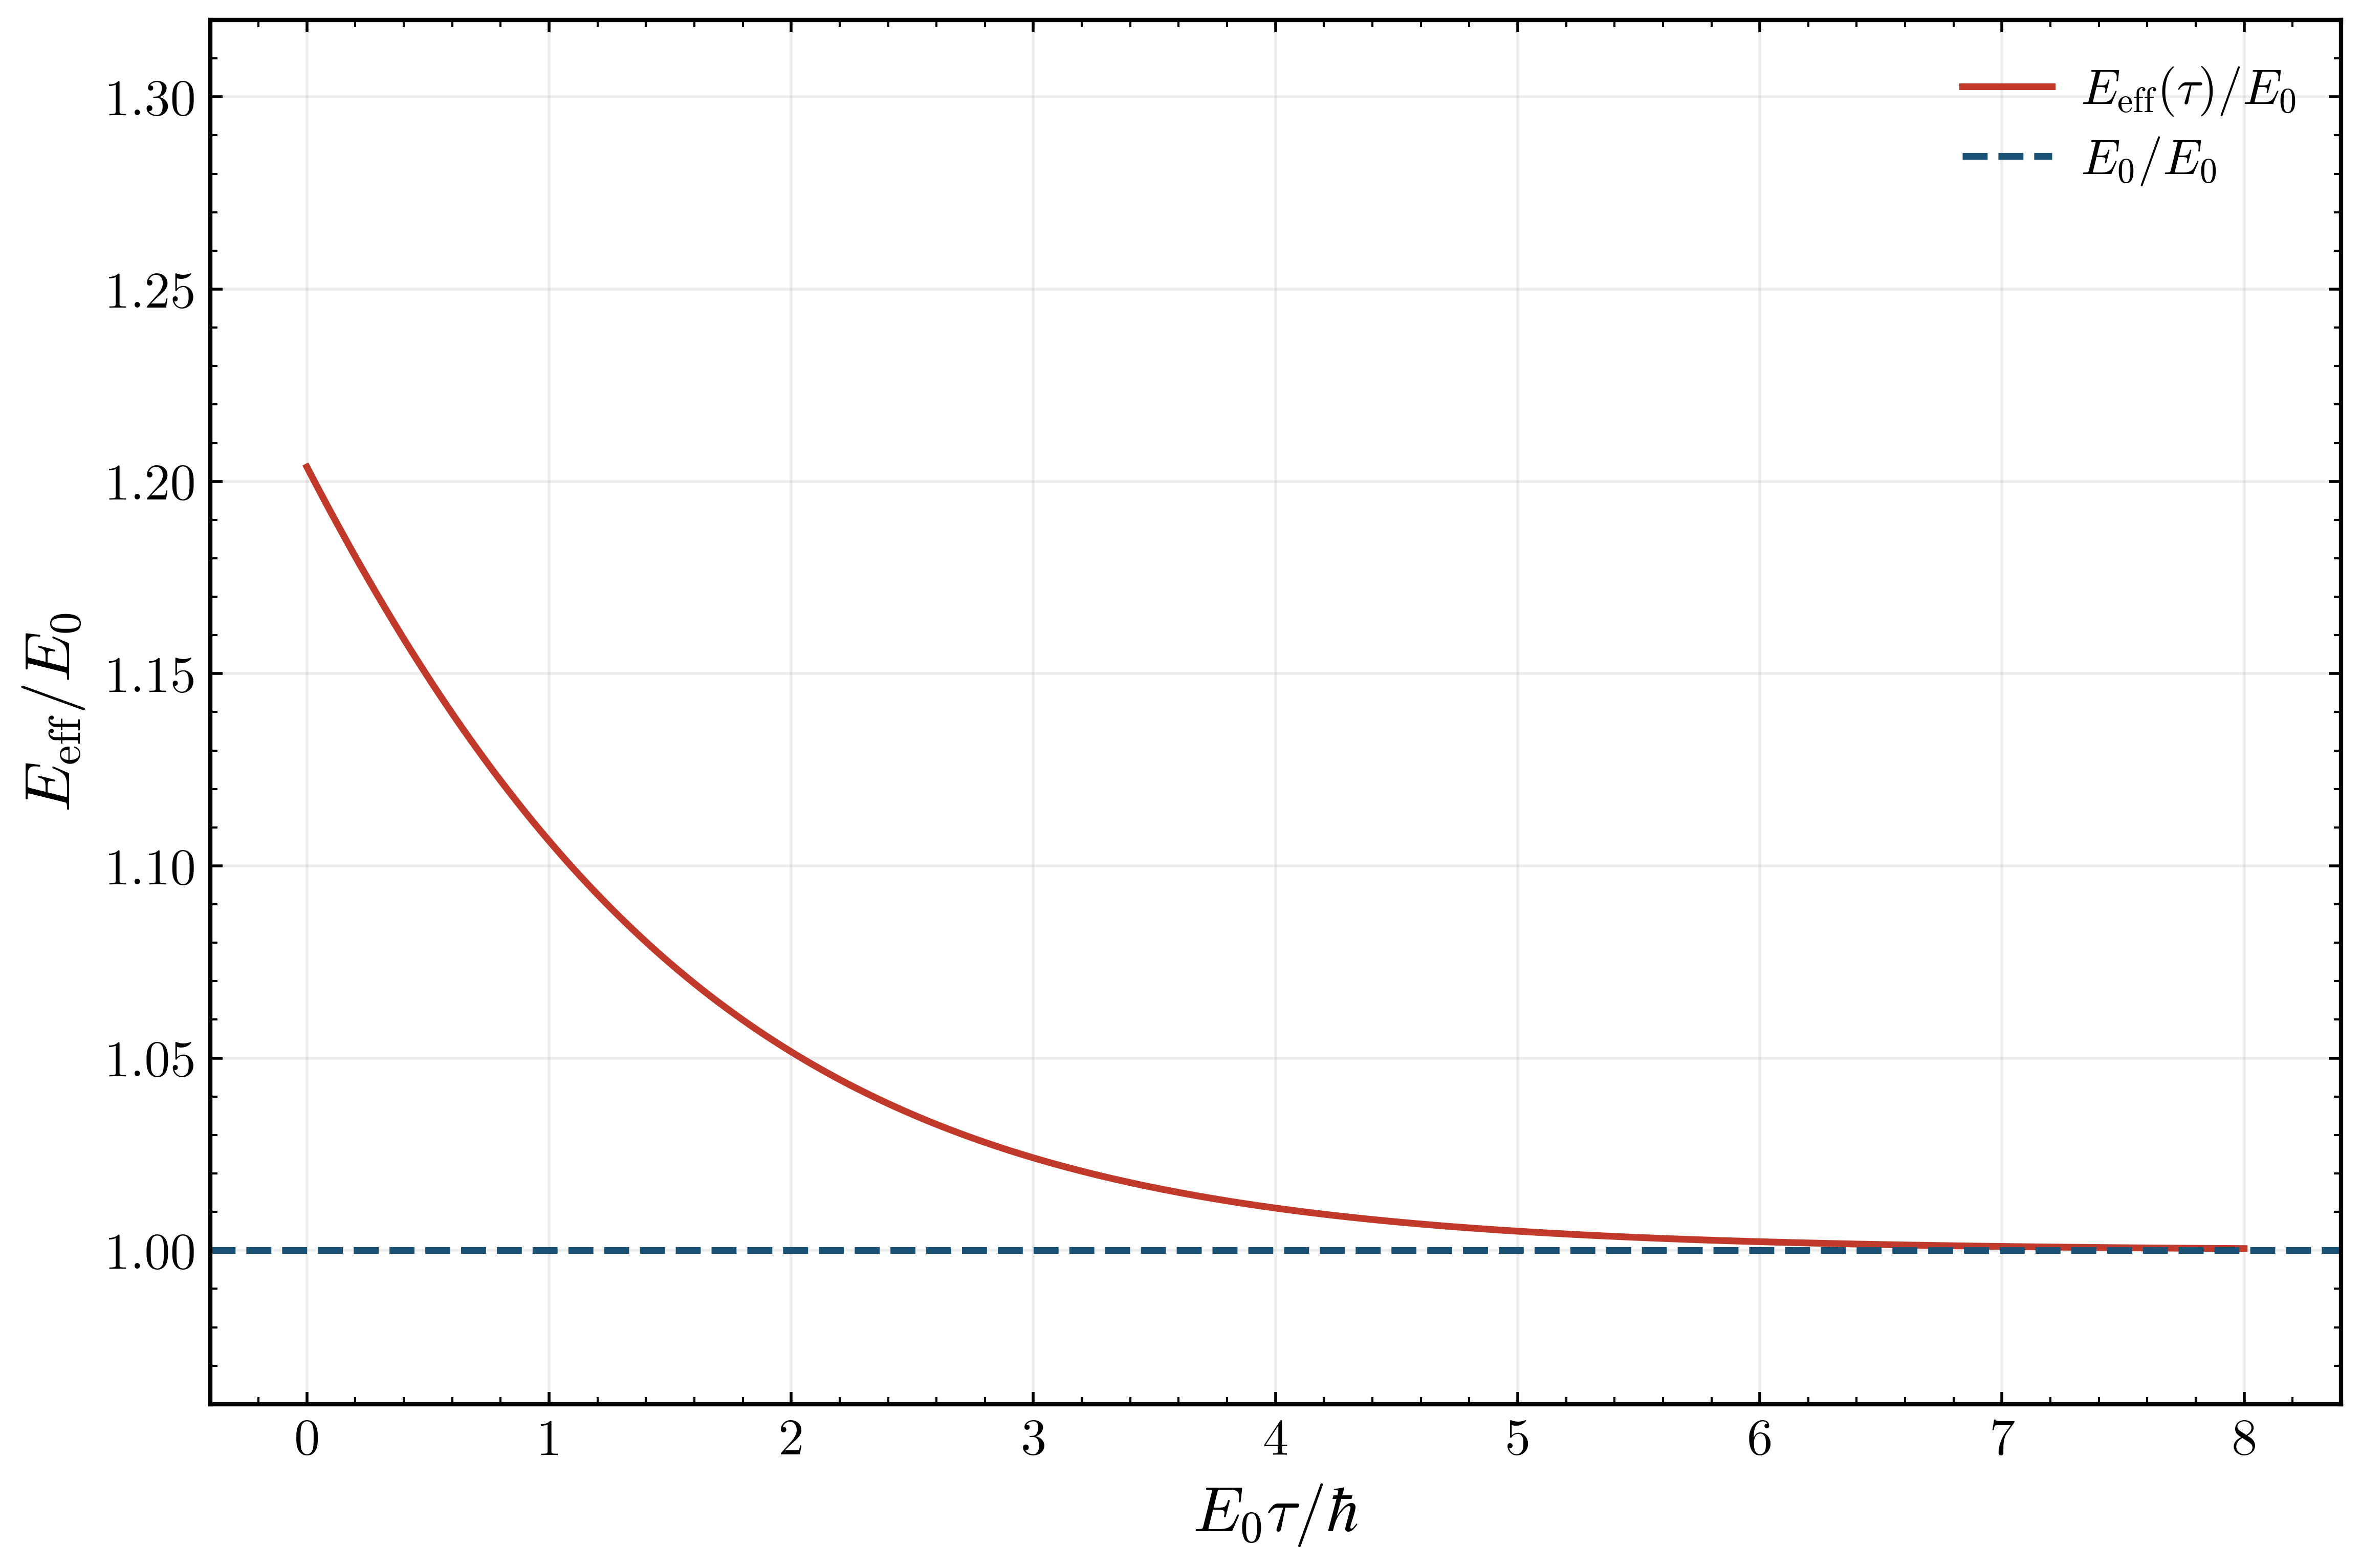
\includegraphics[width=.78\linewidth]{content/FreeElectronQuantumOptics/figures/generated/qcd_euclidean_effective_energy_dp31.png}
 \caption{两态欧几里得关联函数的有效能量示意。横轴和纵轴均按基态能量 $E_0$ 无量纲化；较小 $\tau$ 区域含明显激发态污染，而 $E_{\rm eff}/E_0\to1$ 的平台给出基态能量。曲线由\eqnrefs{eq:qcd-euclidean-effective-energy-dp31} 直接计算。}
 \label{fig:qcd-euclidean-effective-energy-dp31}
\end{figure}

高能 QCD 用重整化微扰理论、重整化群和因子化组织可计算展开；低能区则回到规范不变的欧几里得路径积分。链变量与格元给出保持规范不变性的调节器，Wilson 环给出静态势，拓扑扇区给出非解析半经典结构，Dirac 谱给出手征凝聚，领先手征有效作用量把凝聚连接到轻介子谱，欧几里得关联函数再把这些母定义连接到实际强子能级。禁闭、手征对称性破缺和拓扑效应彼此相关，但没有任何一个能够由“一圈耦合变大”单独推出。


\begin{derivation}[从\eqnrefs{eq:wilson-gauge-action-dp11}到\eqnrefs{eq:wilson-continuum-limit-dp11}]
由小闭合路径与曲率的关系，格元满足

\begin{equation*}
 U_{\mu\nu}(x)
 =\exp\!\left[\ii g_sa^2\mathcal F_{\mu\nu}(x)+\order(a^3)\right].
\end{equation*}
展开指数并使用 $\Tr T^a=0$ 与 $\Tr(T^aT^b)=\delta^{ab}/2$，有
\begin{align*}
 \Re\Tr U_{\mu\nu}
 &=N_c-
 \frac{g_s^2a^4}{2}
 \Tr\!\left(\mathcal F_{\mu\nu}\mathcal F_{\mu\nu}\right)
 +\order(a^6),\\
 &=N_c-
 \frac{g_s^2a^4}{4}
 \mathcal F_{\mu\nu}^a\mathcal F_{\mu\nu}^a
 +\order(a^6).
\end{align*}
代入\eqnrefs{eq:wilson-gauge-action-dp11}，并用 $\beta_{\rm lat}=2N_c/g_s^2$，得到
\begin{equation*}
 \frac{S_W}{\hbar}
 =\sum_xa^4\sum_{\mu<\nu}
 \frac12\mathcal F_{\mu\nu}^a\mathcal F_{\mu\nu}^a
 +\order(a^2).
\end{equation*}
反对称性给
\begin{equation*}
 \sum_{\mu<\nu}\mathcal F_{\mu\nu}^2
 =\frac12\sum_{\mu,\nu}\mathcal F_{\mu\nu}^2,
\end{equation*}
而 Riemann 和在 $a\to0$ 时变成四维积分，因此得到相应的欧几里得 Yang--Mills 连续极限。
\end{derivation}



\begin{derivation}[从\eqnrefs{eq:pontryagin-number-dp11}到\eqnrefs{eq:instanton-action-bound-dp11}]
在四维欧几里得空间定义
\[
({}^\star\!\mathcal F)_{\mu\nu}^a
\equiv\frac12\epsilon_{\mu\nu\rho\sigma}
\mathcal F_{\rho\sigma}^a.
\]
欧几里得号差使 $({}^\star)^2=+1$ 作用在二形式上，并且
\[
({}^\star\!\mathcal F)_{\mu\nu}^a
({}^\star\!\mathcal F)_{\mu\nu}^a
=\mathcal F_{\mu\nu}^a\mathcal F_{\mu\nu}^a.
\]
因此对任一符号都有非负平方
\begin{align*}
0
&\le\frac12\int\dd^4x\,
\bigl(\mathcal F_{\mu\nu}^a
\mp{}^\star\!\mathcal F_{\mu\nu}^a\bigr)^2\\
&=\int\dd^4x\,
\mathcal F_{\mu\nu}^a\mathcal F_{\mu\nu}^a
\mp\int\dd^4x\,
\mathcal F_{\mu\nu}^a{}^\star\!\mathcal F_{\mu\nu}^a.
\end{align*}
选择使第二项与拓扑积分同号的那个符号，便得到
\[
\int\dd^4x\,
\mathcal F_{\mu\nu}^a\mathcal F_{\mu\nu}^a
\ge
\left|
\int\dd^4x\,
\mathcal F_{\mu\nu}^a{}^\star\!\mathcal F_{\mu\nu}^a
\right|.
\]
正文\eqnrefs{eq:pontryagin-number-dp11} 的归一化是
\[
Q_{\rm top}
=\frac{g_s^2}{32\pi^2}
\int\dd^4x\,
\mathcal F_{\mu\nu}^a{}^\star\!\mathcal F_{\mu\nu}^a,
\]
相应的欧几里得 Yang--Mills 作用量为
\[
\frac{S_E}{\hbar}
=\frac14\int\dd^4x\,
\mathcal F_{\mu\nu}^a\mathcal F_{\mu\nu}^a.
\]
两式代入上界，严格得到
\[
\boxed{
\frac{S_E}{\hbar}
\ge\frac{8\pi^2}{g_s^2}|Q_{\rm top}|.}
\]

等号何时成立也不是另加条件：非负平方的积分只有在平方逐点为零时才能饱和，因此
\[
\mathcal F_{\mu\nu}^a
=\pm{}^\star\!\mathcal F_{\mu\nu}^a.
\]
这就是自对偶/反自对偶方程。对 $|Q_{\rm top}|=1$，饱和作用量为 $8\pi^2\hbar/g_s^2$，半经典路径积分权重因而含
\[
\exp\!\left(-\frac{S_E}{\hbar}\right)
=\exp\!\left(-\frac{8\pi^2}{g_s^2}\right),
\]
它在 $g_s=0$ 处具有本质奇点，不能由有限阶耦合常数幂级数产生；这就是“瞬子效应是非微扰的”在数学上的具体含义。
\end{derivation}

\begin{derivation}[从\eqnrefs{eq:qcd-dirac-spectral-density-dp68}到\eqnrefs{eq:banks-casher-dp11}]
正文采用欧几里得 Dirac 算符的反厄米 convention
\begin{equation*}
 \slashed D_E\phi_n=\ii\lambda_n\phi_n,
 \qquad \lambda_n\in\mathbb R,
 \qquad
 \int_{V_4}\dd^4 x\,\phi_m^\dagger\phi_n=\delta_{mn}.
\end{equation*}
无质量算符与 $\gamma^5$ 反对易：
\begin{equation*}
 \{\gamma^5,\slashed D_E\}=0.
\end{equation*}
因此若 $\lambda_n\neq0$，则
\begin{equation*}
 \slashed D_E(\gamma^5\phi_n)
 =-\ii\lambda_n(\gamma^5\phi_n),
\end{equation*}
非零谱严格成 $\pm\lambda$ 对。加入小而正的夸克质量，欧几里得传播子为
\begin{equation*}
 S_E=(\slashed D_E+mc/\hbar)^{-1},
\end{equation*}
因此单味凝聚由 coincident propagator 的迹给出
\begin{equation*}
 -\langle\bar\psi\psi\rangle_m
 =\frac1{V_4}
 \left\langle\Tr\frac1{\slashed D_E+mc/\hbar}\right\rangle.
\end{equation*}
在 $\phi_n$ 本征基中插入完备关系：
\begin{equation*}
 \Tr\frac1{\slashed D_E+mc/\hbar}
 =\sum_n\frac1{\ii\lambda_n+mc/\hbar}.
\end{equation*}
对每一对非零本征值 $\pm\lambda$，
\begin{align*}
 \frac1{\ii\lambda+mc/\hbar}
 +\frac1{-\ii\lambda+mc/\hbar}
 &=\frac{2mc/\hbar}{\lambda^2+(mc/\hbar)^2}.
\end{align*}
于是
\begin{equation*}
 -\langle\bar\psi\psi\rangle_m
 =\frac1{V_4}\left\langle
 \frac{N_0}{mc/\hbar}
 +\sum_{\lambda_n>0}
 \frac{2mc/\hbar}{\lambda_n^2+(mc/\hbar)^2}
 \right\rangle,
\end{equation*}
其中 $N_0$ 是严格零模数。固定拓扑荷时 $N_0=O(1)$，故先取 $V_4\to\infty$ 后 $N_0/V_4\to0$；自发凝聚来自零点附近数目随体积成比例增长的近零模，而不是有限个拓扑零模。

按正文\eqnrefs{eq:qcd-dirac-spectral-density-dp68}，热力学极限把全谱离散求和变成
\begin{equation*}
 \lim_{V_4\to\infty}
 \frac1{V_4}\left\langle\sum_n f(\lambda_n)\right\rangle
 =\int_{-\infty}^{+\infty}\dd\lambda\,\rho(\lambda)f(\lambda).
\end{equation*}
由于 $\rho(-\lambda)=\rho(\lambda)$，传播子迹中的奇函数部分积分为零，只剩
\begin{equation*}
 -\langle\bar\psi\psi\rangle_m
 =\int_{-\infty}^{+\infty}\dd\lambda\,
 \rho(\lambda)
 \frac{mc/\hbar}{\lambda^2+(mc/\hbar)^2}.
\end{equation*}
令 $\epsilon=mc/\hbar$。对任意在零点连续的谱密度，分布极限
\begin{equation*}
 \lim_{\epsilon\to0^+}
 \frac{\epsilon}{\lambda^2+\epsilon^2}
 =\pi\delta(\lambda)
\end{equation*}
直接给出
\begin{align*}
 -\lim_{m\to0^+}\lim_{V_4\to\infty}
 \langle\bar\psi\psi\rangle_m
 &=\pi\int_{-\infty}^{+\infty}\dd\lambda\,
 \rho(\lambda)\delta(\lambda)\\
 &=\pi\rho(0),
\end{align*}
即正文\eqnrefs{eq:banks-casher-dp11}。若有 $N_f$ 个简并轻味，则每个味都满足同一关系，而味求和的凝聚相应多出因子 $N_f$。若把极限顺序反过来，有限体积谱仍是离散的，除有限个拓扑零模外没有连续的零点谱密度；因此 $V_4\to\infty$ 必须先于 $m\to0^+$，这正是自发对称性破缺所需的热力学极限。
\end{derivation}

\begin{derivation}[从\eqnrefs{eq:qcd-chiral-lo-action-dp33}到\eqnrefs{eq:qcd-gmor-dp33}]
取两轻味同位旋极限，并把

\begin{equation*}
 U=\exp\!\left(\frac{\ii\pi}{F_\pi}\right),
 \qquad
 \pi=\pi^a\tau^a,
 \qquad
 \Tr(\tau^a\tau^b)=2\delta^{ab}.
\end{equation*}
展开到二次阶，
\begin{align*}
 U&=1+\frac{\ii\pi}{F_\pi}-\frac{\pi^2}{2F_\pi^2}+\order(\pi^3),\\
 U^\dagger&=1-\frac{\ii\pi}{F_\pi}-\frac{\pi^2}{2F_\pi^2}+\order(\pi^3).
\end{align*}
动能项因而变成
\begin{align*}
 \frac{F_\pi^2}{4(\hbar c)^2}
 \Tr(\partial_\mu U^\dagger\partial^\mu U)
 &=\frac1{4(\hbar c)^2}
 \Tr(\partial_\mu\pi\,\partial^\mu\pi)+\order(\pi^4),\\
 &=\frac1{2(\hbar c)^2}
 \partial_\mu\pi^a\partial^\mu\pi^a+\order(\pi^4),
\end{align*}
得到三个规范归一化的实标量低能模。

质量矩阵在同位旋极限中为 $M_q=\hat m c^2 I_2$，其中 $\hat m=(m_u+m_d)/2$。线性 \(\pi\) 介子项在 $U+U^\dagger$ 中相消，而二次项给
\begin{align*}
 \Tr[M_q(U^\dagger+U)]
 &=4\hat m c^2
 -\frac{\hat m c^2}{F_\pi^2}\Tr(\pi^2)+\order(\pi^4),\\
 &=4\hat m c^2
 -\frac{2\hat m c^2}{F_\pi^2}\pi^a\pi^a+\order(\pi^4).
\end{align*}
代回\eqnrefs{eq:qcd-chiral-lo-action-dp33}，二次质量项为
\begin{equation*}
 -\frac{B_0\hat m c^2}{(\hbar c)^4}\pi^a\pi^a.
\end{equation*}
与标准二次作用量中的
\begin{equation*}
 -\frac{m_\pi^2c^4}{2(\hbar c)^4}\pi^a\pi^a
\end{equation*}
比较，得到
\begin{equation*}
 m_\pi^2c^4=2B_0\hat m c^2=B_0(m_u+m_d)c^2.
\end{equation*}
最后使用已定义的低能常数匹配
\begin{equation*}
 B_0=-\frac{(\hbar c)^3\langle\bar q q\rangle}{F_\pi^2},
\end{equation*}
即可得到\eqnrefs{eq:qcd-gmor-dp33}。该关系的修正由更高阶轻夸克质量插入与手征圈图共同控制，其相对大小按\eqnrefs{eq:qcd-chiral-control-dp33} 的幂次计数组织。
\end{derivation}


